% Options for packages loaded elsewhere
\PassOptionsToPackage{unicode}{hyperref}
\PassOptionsToPackage{hyphens}{url}
%
\documentclass[
  a4paper,
]{scrbook}

\usepackage{amsmath,amssymb}
\usepackage{iftex}
\ifPDFTeX
  \usepackage[T1]{fontenc}
  \usepackage[utf8]{inputenc}
  \usepackage{textcomp} % provide euro and other symbols
\else % if luatex or xetex
  \usepackage{unicode-math}
  \defaultfontfeatures{Scale=MatchLowercase}
  \defaultfontfeatures[\rmfamily]{Ligatures=TeX,Scale=1}
\fi
\usepackage{lmodern}
\ifPDFTeX\else  
    % xetex/luatex font selection
  \setmainfont[]{Latin Modern Roman}
  \setsansfont[]{Latin Modern Roman}
\fi
% Use upquote if available, for straight quotes in verbatim environments
\IfFileExists{upquote.sty}{\usepackage{upquote}}{}
\IfFileExists{microtype.sty}{% use microtype if available
  \usepackage[]{microtype}
  \UseMicrotypeSet[protrusion]{basicmath} % disable protrusion for tt fonts
}{}
\makeatletter
\@ifundefined{KOMAClassName}{% if non-KOMA class
  \IfFileExists{parskip.sty}{%
    \usepackage{parskip}
  }{% else
    \setlength{\parindent}{0pt}
    \setlength{\parskip}{6pt plus 2pt minus 1pt}}
}{% if KOMA class
  \KOMAoptions{parskip=half}}
\makeatother
\usepackage{xcolor}
\setlength{\emergencystretch}{3em} % prevent overfull lines
\setcounter{secnumdepth}{5}
% Make \paragraph and \subparagraph free-standing
\ifx\paragraph\undefined\else
  \let\oldparagraph\paragraph
  \renewcommand{\paragraph}[1]{\oldparagraph{#1}\mbox{}}
\fi
\ifx\subparagraph\undefined\else
  \let\oldsubparagraph\subparagraph
  \renewcommand{\subparagraph}[1]{\oldsubparagraph{#1}\mbox{}}
\fi


\providecommand{\tightlist}{%
  \setlength{\itemsep}{0pt}\setlength{\parskip}{0pt}}\usepackage{longtable,booktabs,array}
\usepackage{calc} % for calculating minipage widths
% Correct order of tables after \paragraph or \subparagraph
\usepackage{etoolbox}
\makeatletter
\patchcmd\longtable{\par}{\if@noskipsec\mbox{}\fi\par}{}{}
\makeatother
% Allow footnotes in longtable head/foot
\IfFileExists{footnotehyper.sty}{\usepackage{footnotehyper}}{\usepackage{footnote}}
\makesavenoteenv{longtable}
\usepackage{graphicx}
\makeatletter
\def\maxwidth{\ifdim\Gin@nat@width>\linewidth\linewidth\else\Gin@nat@width\fi}
\def\maxheight{\ifdim\Gin@nat@height>\textheight\textheight\else\Gin@nat@height\fi}
\makeatother
% Scale images if necessary, so that they will not overflow the page
% margins by default, and it is still possible to overwrite the defaults
% using explicit options in \includegraphics[width, height, ...]{}
\setkeys{Gin}{width=\maxwidth,height=\maxheight,keepaspectratio}
% Set default figure placement to htbp
\makeatletter
\def\fps@figure{htbp}
\makeatother

\usepackage{booktabs}
\usepackage{longtable}
\usepackage{array}
\usepackage{multirow}
\usepackage{wrapfig}
\usepackage{float}
\usepackage{colortbl}
\usepackage{pdflscape}
\usepackage{tabu}
\usepackage{threeparttable}
\usepackage{threeparttablex}
\usepackage[normalem]{ulem}
\usepackage{makecell}
\usepackage{xcolor}
\usepackage{fancyhdr}
\usepackage{titling}
\usepackage{pdflscape}
\usepackage{geometry}
\setlength{\droptitle}{-2cm}
\preauthor{
  \begin{center}
  \Large
  \vspace{10mm}
  by
  \vspace{20mm}
}
\postauthor{
  \end{center}
  \vfill
}

\predate{
  \begin{center}
  A thesis 
  submitted in partial fulfilment of the \\
  requirements of the degree of \\
  Doctor of Philosophy in Physics\\               % Degree
  School of Physical and Chemical Sciences\\          % Department
  Te Herenga Waka - Victoria University of Wellington\\                       % University 
  \vspace{5mm}
}
\postdate{
  \\
  
\includegraphics[width=3in,height=1.5in]{figures/VUW-logo.png}\\
  \end{center}
  }

\renewcommand{\topfraction}{.8}
\renewcommand{\bottomfraction}{.7}
\renewcommand{\textfraction}{.15}
\renewcommand{\floatpagefraction}{.8}
\setcounter{topnumber}{3}
\setcounter{bottomnumber}{3}
\setcounter{totalnumber}{4}

\clubpenalty=9996
\widowpenalty=9999
\makeatletter
\makeatother
\makeatletter
\@ifpackageloaded{bookmark}{}{\usepackage{bookmark}}
\makeatother
\makeatletter
\@ifpackageloaded{caption}{}{\usepackage{caption}}
\AtBeginDocument{%
\ifdefined\contentsname
  \renewcommand*\contentsname{Table of contents}
\else
  \newcommand\contentsname{Table of contents}
\fi
\ifdefined\listfigurename
  \renewcommand*\listfigurename{List of Figures}
\else
  \newcommand\listfigurename{List of Figures}
\fi
\ifdefined\listtablename
  \renewcommand*\listtablename{List of Tables}
\else
  \newcommand\listtablename{List of Tables}
\fi
\ifdefined\figurename
  \renewcommand*\figurename{Figure}
\else
  \newcommand\figurename{Figure}
\fi
\ifdefined\tablename
  \renewcommand*\tablename{Table}
\else
  \newcommand\tablename{Table}
\fi
}
\@ifpackageloaded{float}{}{\usepackage{float}}
\floatstyle{ruled}
\@ifundefined{c@chapter}{\newfloat{codelisting}{h}{lop}}{\newfloat{codelisting}{h}{lop}[chapter]}
\floatname{codelisting}{Listing}
\newcommand*\listoflistings{\listof{codelisting}{List of Listings}}
\makeatother
\makeatletter
\@ifpackageloaded{caption}{}{\usepackage{caption}}
\@ifpackageloaded{subcaption}{}{\usepackage{subcaption}}
\makeatother
\makeatletter
\@ifpackageloaded{tcolorbox}{}{\usepackage[skins,breakable]{tcolorbox}}
\makeatother
\makeatletter
\@ifundefined{shadecolor}{\definecolor{shadecolor}{rgb}{.97, .97, .97}}
\makeatother
\makeatletter
\makeatother
\makeatletter
\makeatother
\ifLuaTeX
  \usepackage{selnolig}  % disable illegal ligatures
\fi
\usepackage[citestyle = ieee,urldate = iso8601]{biblatex}
\addbibresource{references.bib}
\IfFileExists{bookmark.sty}{\usepackage{bookmark}}{\usepackage{hyperref}}
\IfFileExists{xurl.sty}{\usepackage{xurl}}{} % add URL line breaks if available
\urlstyle{same} % disable monospaced font for URLs
\hypersetup{
  pdftitle={Developing an Insect Odorant Receptor Bioelectronic Nose for Vapour-Phase Detection},
  pdfauthor={Eddyn Oswald Perkins Treacher},
  hidelinks,
  pdfcreator={LaTeX via pandoc}}

\title{Developing an Insect Odorant Receptor Bioelectronic Nose for
Vapour-Phase Detection}
\author{Eddyn Oswald Perkins Treacher}
\date{Dec 2024}

\begin{document}
\frontmatter

\maketitle

\clearpage
\newpage
\thispagestyle{empty} % Hide header and footer on this page
\mbox{~}
\clearpage
\newpage

%----------------------------------------------
%   Abstract
%----------------------------------------------

\thispagestyle{plain}

\begin{flushleft}
% Manually add a section to the table of contents
\pagenumbering{roman}
\addcontentsline{toc}{chapter}{Abstract}
\huge\textbf{Abstract}
\end{flushleft}

\vspace*{\baselineskip}

The ability to detect volatile organic compounds in a highly sensitive and selective manner is desirable for applications as varied as diagnosis of illnesses at a remote clinic, monitoring of air in an industrial setting, or identification of invasive organisms at a biosecurity checkpoint. Historically, animal noses have been used for such tasks, as their combined sensitivity and selectivity are superior to traditional artificial sensors. However, training and deploying animals in such situations is both time and cost intensive. In recent years, an improved understanding of \textit{in vivo} biological sensing has driven efforts to mimic these highly efficient processes in an artificial sensor format. \\[5pt] To this end, a “bioelectronic nose” was developed. This sensor uses an artificial transducer to amplify responses of an insect odorant receptor protein to specific volatile compounds. Thin-film transistors were used as the amplifier element, given their low cost, small size and extreme sensitivity. Various thin-film morphologies were compared, and their suitability for bioelectronic nose development assessed. Transducers made using a novel steam-assisted thin-film deposition technique were found to have highly consistent device-to-device electrical properties relative to other films. Films made using this process typically showed more surface contamination than other morphologies, but their high sensitivity was nonetheless confirmed with a non-specific sensing series in an aqueous environment. \\[5pt] One of the major challenges encountered in this thesis was variability in the quality of sensor functionalisation. Raman spectroscopy and fluorescence microscopy confirmed an existing non-covalent attachment method could successfully immobilise nanodiscs onto the transistor channel region. However, various sensors functionalised using the same procedure often exhibited no sensing activity. Extensive electrical characterisation indicated the presence of an unidentified contamination layer preventing electrical interaction between the insect odorant receptors and transducer thin-film. It was shown that this layer was unlikely to be directly associated with the thin-film morphology used for the transducer. \\[5pt] Subsequently, an alternative biotin-based non-covalent method was used for functionalisation of the proteins, which eliminated several possible contamination sources. This alternative biotin-based method was used to demonstrate successful aqueous sensing of femtomolar concentrations of methyl salicylate by an iOR10a-functionalised device. When tested in a custom-built vapour delivery system, a similar bioelectronic sensor was shown to be highly sensitive to the target vapour. However, consistent reproduction of the biotin-based method was challenging due to the harsh cleaning method involved. It was therefore difficult to determine conclusively whether sensor responses were selective. By finding new, systematic approaches to address the major barriers to sensor success carefully identified in this work, there are promising signs that a highly reliable vapour-phase bioelectronic nose can be produced.

%\fancyhf{} %clear all headers and footers fields
%\thispagestyle{fancy} % Change header and footer on this page
%\renewcommand{\headrulewidth}{0pt}
%\fancyhead[L]{\textit{Abstract}} % Set header content
%\fancyfoot[L]{\thepage} %prints the page number on the right side of the header

\clearpage
\newpage
\thispagestyle{empty} % Hide header and footer on this page
\mbox{~}
\clearpage
\newpage


%----------------------------------------------
%   Acknowledgement
%----------------------------------------------

\thispagestyle{plain}

\begin{flushleft}
% Manually add a section to the table of contents
\addcontentsline{toc}{chapter}{Acknowledgements}
\huge\textbf{Acknowledgements}
\end{flushleft}

\vspace*{\baselineskip}

I would first like to acknowledge the lands of my ancestors, and the lands of the sovereign first peoples to which my ancestors travelled. We each come from the land, live off the land and return to the land.\\[5pt]
\textit{Noon of Essex to Warrang, on the Friends, Autumn 1811} \\[5pt]
\textit{Cave of Cambridgeshire to Warrang, on the Royal Charlotte, Autumn 1825} \\[5pt]
\textit{Boyce of Suffolk to Warrang, 1832} \\[5pt] 
\textit{Charlton of Northumberland to Warrang, on the Clyde, Spring 1834} \\[5pt]
\textit{Prouse of Devonshire to Pito-one, on the Duke of Roxburgh, Summer 1840} \\[5pt]
\textit{Ebden of Devonshire to Pito-one, on the Tyne, Winter 1841} \\[5pt]
\textit{Collis of Hampshire to Pito-one, on the Birman, Autumn 1842} \\[5pt]
\textit{Swann of Loch Garman to Te Whanganui-a-Tara, 1844} \\[5pt] 
\textit{Blythe of Berkshire to Whakatū, circa 1846} \\[5pt]
\textit{Innes of Berkshire to Naarm, on the Sacramento, Autumn 1853} \\[5pt]
\textit{Sheppard of Gloucestershire to Naarm, 1853} \\[5pt] 
\textit{Bruce of London to Naarm, on the Omega, Autumn 1855} \\[5pt]
\textit{Quennell of Surrey to Warrang, on the Asiatic, Winter 1855} \\[5pt]
\textit{Barr of Glasgow to Kōpūtai, on the Sir Edward Paget, Winter 1856} \\[5pt] 
\textit{Perkins of London to Te Whanganui-a-Tara, on the Matoaka, Spring 1859} \\[5pt]
\textit{McKee of Antrim to Tāmaki Makaurau, on the Indian Empire, Spring 1862} \\[5pt]
\textit{Sandilands of Peeblesshire to Ōtepoti, circa 1864} \\[5pt] 
\textit{Treacher of Berkshire to Te Whanganui-a-Tara, on the Wild Duck, Summer 1865} \\[5pt]
\textit{McTaggart of Argyllshire to Kōpūtai, on the Edward P. Bouverie, Autumn 1869} \\[5pt] 
\textit{Chapman of Kent to Whakatū, on the Adamant, Winter 1874} \\[5pt]
\textit{Cheel of London to Whakatū, on the Queen Bee, Winter 1877} \\[5pt]  
\textit{Hutchison of Aberdeen to Tarntanya, before 1882.} \\[5pt] 
I chose to start my doctoral studies just a few months into a global pandemic. Completing a challenging project with a worldwide crisis in the background might have been impossible without the supervision of AProf. Natalie Plank. Her ability to adapt to and overcome any problem has taught me that there is no situation which is truly unmanageable. I am deeply grateful for her leadership throughout a time of particular chaos. \newpage
\fancyhf{} %clear all headers and footers fields
\thispagestyle{fancy} % Change header and footer on this page
\renewcommand{\headrulewidth}{0pt}
\fancyhead[L]{\textit{Acknowledgements}} % Set header content
\fancyfoot[L]{\thepage} %prints the page number on the left side of the header 
I started this project with minimal formal training in biological science, coming from a primarily physics and engineering background. \\[5pt] The immense support I received from Melissa Jordan and Colm Carraher from the Institute for Plant and Food Research (PFR) to complete this project meant that this was not an issue, and I thank them both immensely for this. \\[5pt] I would not have been able to begin this thesis without the financial backing and support I received from PFR and the Better Border Biosecurity (B3) programme. In particular, I am very grateful to Andrew Kralicek, formerly with PFR and now at Scentian Bio, and the ex-Director of B3, David Teulon, for helping to secure funding for my project. I would also like to thank the donor of the Ernest Marsden Scholarship in Physics for their significant financial support. \\[5pt] There are many incredibly supportive people who I worked alongside during my project. I would like to start off by thanking Rifat Ullah, whose mentoring and kindness encouraged me to pursue further study. His work on the initial design and setup of the vapour delivery system was invaluable to me throughout this project. I am also especially grateful to Alex Puglisi, for constructing the mechanical elements of the vapour delivery system and giving me extensive feedback on the system design. I would like to thank Peter Coard, for his advice and guidance when constructing the electrical elements of the vapour delivery system. I thank Selvan Murugathas, too, for his advice on constructing the insect odorant receptor sensors, as well as Damon Colbert and Valentina Lucarelli, who provided the insect odorant receptor nanodiscs used in this work. \\[5pt] Thank you to AProf. Ben Ruck, my supportive secondary supervisor, and to AProf. Franck Natali, for always asking about my thesis in the tearoom. Thank you to Gideon Gouws for his friendly encouragement and advice. For their substantial technical assistance and mentoring during this project, I thank Alan Rennie, Grant Franklin, Chris Lepper, Rashika Gunasekara, Pete Jebson and Sushila Pillai from VUW, Andrew Chan from PFR, AProf. Charles Unsworth from the University of Auckland, and Prof. Simon Brown and his nanomaterials group from the University of Canterbury. \\[5pt] I was lucky enough to start my doctoral program just as a group of supportive and talented senior students were finishing, and finished just as a group of enthusiastic and talented new doctoral students were starting. A special thanks to Jenna Nyugen, Erica Happe and Erica Cassie for teaching me the fabrication processes and characterisation procedures that made this thesis happen; and a special thanks to Marissa Dierkes, Danica Fontein, Sangar Begzaad and Alireza Zare, for their incredible support throughout the thesis writing process. I am also thankful for the assistance of the cleanroom group interns over the course of my PhD, including Liam, Hayden and Lotte. I would further like to thank everyone else I shared an office with and worked alongside, including Jackson, Will, Roshni, Ali, Sam, Kira, Catherine, Martin, Janani, Ted, Kiri and Joe. \\[5pt] A massive thank you to Openstar Technologies. It has been an honour to work on a cutting-edge plasma physics project right here in Te Whanganui-a-Tara. A particularly big thank you to Ratu, Darren and Thomas for having me as part of the plasma physics team. Thank you also to the other Openstar interns, in particular the other plasma physics interns, Valentina, Benjy and Chris. I wish you success in all your dipole-confined plasma related endeavours. \\[5pt] I want to thank Shodokan Aikido New Zealand for their support throughout this thesis, in particular for the once-in-a-lifetime opportunity to travel to Osaka to be graded for first-dan by Nariyama Shihan. Thanks for all the training and support, Ian. Thank you to all the friends and family, old and new, who have supported me over these wild past few years. You know who you are. \\[5pt] Thank you to my brother, Keeson, and to my parents, Hilary and Phillip. Your support means everything to me, and I would not be where I am today without you. Our Friday lunchtime cafe visits inspired and motivated me throughout the doctoral program. Thank you, thank you, thank you for your love, your compassion, and for being there for me. \\[5pt] Finally, thank you Nina. Your love has kept me going through the most difficult and most wonderful times over the last three and a half years. You are the light of my life, and I am so happy to have taken on this challenge with you by my side. \\[5pt] Arohanui and peace to you all, Eddyn (Ned)

\fancyhf{} %clear all headers and footers fields
\thispagestyle{fancy} % Change header and footer on this page
\renewcommand{\headrulewidth}{0pt}
\fancyhead[R]{\textit{Acknowledgements}} % Set header content
\fancyfoot[R]{\thepage} %prints the page number on the right side of the header

\clearpage
\newpage
\thispagestyle{empty} % Hide header and footer on this page
\mbox{~}
\clearpage
\newpage

\pagestyle{headings}

\ifdefined\Shaded\renewenvironment{Shaded}{\begin{tcolorbox}[sharp corners, frame hidden, enhanced, interior hidden, boxrule=0pt, breakable, borderline west={3pt}{0pt}{shadecolor}]}{\end{tcolorbox}}\fi

\renewcommand*\contentsname{Table of Contents}
{
\setcounter{tocdepth}{2}
\addcontentsline{toc}{chapter}{Table of Contents}
\tableofcontents
}
\listoffigures
\addcontentsline{toc}{chapter}{List of Figures}
\listoftables
\addcontentsline{toc}{chapter}{List of Tables}

\clearpage
\newpage
\thispagestyle{empty} % Hide header and footer on this page
\mbox{~}
\clearpage
\newpage

%----------------------------------------------
%   List of Abbreviations
%----------------------------------------------

\thispagestyle{plain}

\begin{flushleft}
% Manually add a section to the table of contents
\addcontentsline{toc}{chapter}{List of Abbreviations}
\huge\textbf{List of Abbreviations}
\end{flushleft}

\vspace*{\baselineskip}

\begin{table}[H]
  \begin{tabular}{@{}p{0.25\textwidth} p{0.75\textwidth}@{}}  % Adjust the width as needed
    2D  & 2-Dimensional  \\[5pt]
    Ab  & Antibody  \\[5pt]
    AB  & Amyl Butyrate  \\[5pt]
    AB-NTA  & N$\alpha$,N$\alpha$-Bis(carboxymethyl)-\textit{L}-lysine hydrate  \\[5pt]
    AFM  & Atomic Force Microscope/Microscopy  \\[5pt]
    AH  & Absolute Humidity  \\[5pt]
    Avi-tag  & Avidin-tag  \\[5pt]
    BMIM  & 1-butyl-3-methylimidazolium bis(trifluoromethylsulfonyl)imide  \\[5pt]
    BWF  & Breit-Wigner-Fano  \\[5pt]
    CAD  & Computer Aided Design \\[5pt]
    CNT  & Carbon Nanotube  \\[5pt]
    CVD  & Chemical Vapour Deposition  \\[5pt]
    Cy3  & Cyanine 3  \\[5pt]
    DAN  & 1,5-diaminonaphthalene  \\[5pt]
    DAQ  & Data Acquisition Input/Output Module  \\[5pt]
    DCB  & 1,2-dichlorobenzene  \\[5pt]
    DI  & Deionised  \\[5pt]
    DMF  & Dimethylformamide   \\[5pt]
    DMSO  & Dimethylsulfoxide   \\[5pt]
    DMT-MM   & 4-(4,6-dimethoxy-1,3,5-triazin-2-yl)-4 methylmorpholinium chloride \\[5pt]
    DMMP  & Dimethyl Methylphosphonate  \\[5pt]
    DNA  & Deoxyribonucleic Acid  \\[5pt]
    E2Hex  & \textit{trans}-2-hexan-1-al  \\[5pt]
    EB  & Ethyl Butyrate  \\[5pt]
    EDC  & 1-Ethyl-3-(3-dimethylaminopropyl)carbodiimide  \\[5pt]
    EDL  & Electric Double Layer  \\[5pt]
    EIS  & Electrochemical Impedance Spectroscopy  \\[5pt]
    EtHex  & Ethyl Hexanoate  \\[5pt]
  \end{tabular}
\end{table}

\newpage
\fancyhf{} %clear all headers and footers fields
\thispagestyle{fancy} % Change header and footer on this page
\renewcommand{\headrulewidth}{0pt}
\fancyhead[L]{\textit{List of Abbreviations}} % Set header content
\fancyfoot[L]{\thepage} %prints the page number on the right side of the header
\begin{table}[H]
  \begin{tabular}{@{}p{0.25\textwidth} p{0.75\textwidth}@{}}  % Adjust the width as needed
    EtOH  & Ethanol  \\[5pt]
    FET  & Field-Effect Transistor  \\[5pt]
    FITC  & Fluorescein isothiocyanate  \\[5pt]
    GA  & Glutaraldehyde  \\[5pt]
    GFET  & Graphene Field-Effect Transistor  \\[5pt]
    GFP  & Green Fluorescent Protein  \\[5pt]
    GPCR  & G-protein Coupled Receptor  \\[5pt]
    HEK  & Human Embryonic Kidney  \\[5pt]
    His-tag  & Histidine-tag  \\[5pt]
    hOR  & Human Odorant Receptor  \\[5pt]
    HPLC  & High-performance Liquid Chromatography   \\[5pt]
    iOR  & Insect Odorant Receptor  \\[5pt]
    IPA  & Isopropanol  \\[5pt]
    LOD  & Limit of Detection  \\[5pt]
    m-CNT  & Metallic Carbon Nanotube   \\[5pt]
    MeOH  & Methanol   \\[5pt]
    MeSal  & Methyl Salicylate   \\[5pt]
    MFC  & Mass Flow Controller   \\[5pt]
    mOR  & Mouse Odorant Receptor  \\[5pt]
    MOSFET  & Metal-Oxide-Semiconductor Field-Effect Transistor  \\[5pt]
    MSP  & Membrane Scaffold Protein  \\[5pt]
    MWCNT  & Multi-Walled Carbon Nanotube  \\[5pt]
    ND  & Nanodisc  \\[5pt]
    NHS  & N-Hydroxysuccinimide  \\[5pt]
    NHSS  & N-hydroxysulfosuccinimide   \\[5pt]
    NMR  & Nuclear Magnetic Resonance  \\[5pt]
    NSB  & Non-Specific Binding   \\[5pt]
    NTA  & Nitrilotriacetic Acid   \\[5pt]
    OBP  & Odorant Binding Protein  \\[5pt]
    OR  & Odorant Receptor  \\[5pt]
    ORCO  & Odorant Receptor Co-Receptor  \\[5pt]
  \end{tabular}
\end{table}

\newpage
\fancyhf{} %clear all headers and footers fields
\thispagestyle{fancy} % Change header and footer on this page
\renewcommand{\headrulewidth}{0pt}
\fancyhead[R]{\textit{List of Abbreviations}} % Set header content
\fancyfoot[R]{\thepage} %prints the page number on the right side of the header
\begin{table}[H]
  \begin{tabular}{@{}p{0.25\textwidth} p{0.75\textwidth}@{}}  % Adjust the width as needed
    PBA  & 1-Pyrenebutyric Acid  \\[5pt]
    PBASE  & 1-Pyrenebutanoic Acid N-hydroxysuccinimide Ester  \\[5pt]
    PBS  & Phosphate-Buffered Saline  \\[5pt]
    PCB  & Printed Circuit Board   \\[5pt]
    PDL & Poly-\textit{D}-lysine  \\[5pt]
    PDMS  & Polydimethylsiloxane   \\  [5pt]
    PEG  & Polyethylene Glycol  \\[5pt] 
    PID  & Photoionisation Detector  \\[5pt] 
    PLL  & Poly-\textit{L}-lysine  \\[5pt]
    PPB  & Pyrene-PEG-Biotin  \\[5pt]
    PPF  & Pyrene-PEG-FITC  \\[5pt]
    PPN  & Pyrene-PEG-NTA  \\[5pt]
    PPR  & Pyrene-PEG-Rhodamine  \\[5pt]
    PTFE  & Polytetrafluoroethylene (Teflon™)  \\[5pt]
    PVC  & Polyvinyl chloride  \\[5pt]
    QCM  & Quartz Crystal Microbalance  \\[5pt]
    RH  & Relative Humidity  \\[5pt]
    RHI  & Relative Humidity and Temperature Indicator  \\[5pt] 
    RNA  & Ribonucleic Acid   \\[5pt]
    SAW  & Surface Acoustic Wave   \\[5pt]
    s-CNT  & Semiconducting Carbon Nanotube   \\[5pt]
    SEM  & Scanning Electron Microscope/Microscopy   \\[5pt]
    SMU  & Source Measure Unit   \\[5pt]
    SPR  & Surface Plasmon Resonance   \\[5pt]
    SWCNT  & Single-Walled Carbon Nanotube   \\[5pt]
    TFTFET  & Thin-Film Field-Effect Transistor  \\[5pt]
    TMAH  & Tetramethylammonium hydroxide  \\[5pt]
    TX  & Transfer Characteristics  \\[5pt]
    UV  & Ultraviolet  \\[5pt]
    VI  & Virtual Instrument  \\[5pt]
    VUAA1  & N-(4-Ethylphenyl)-2-{[4-ethyl-5-(pyridin-3-yl)-4H-1,2,4-triazol-3-yl]sulfanyl}acetamide  \\[5pt] 
  \end{tabular}
\end{table}

\clearpage
\newpage
\thispagestyle{empty} % Hide header and footer on this page
\mbox{~}
\clearpage
\newpage

% Adjust the top and bottom margins of float pages to center floats
\makeatletter
\setlength{\@fptop}{0pt plus 1fil}
\setlength{\@fpbot}{0pt plus 1fil}
\makeatother

\pagestyle{headings}
\mainmatter
\bookmarksetup{startatroot}

\hypertarget{introduction}{%
\chapter{Introduction}\label{introduction}}

\hypertarget{background}{%
\section{Background}\label{background}}

The `bioelectronic nose', an electronic transducer modified with
elements of the animal olfactory system, has the potential to allow
specific detection of airborne volatile compounds at concentrations as
low as parts per trillion
\autocite{Glatz2011,Kwon2015,Dung2018,Kim2022a}. An ideal transducer
platform is the thin-film transistor (TFT) which is particularly
portable, simple to use, small and robust
\autocite{Kauffman2008,Khan2020}. The thin films used in these
field-effect transistors (FETs) include carbon nanotube networks and
graphene, low-dimensional nanomaterials which are both highly sensitive
and biocompatible \autocite{Shkodra2021}. The implications of successful
development of such a portable and robust bioelectronic nose are
significant. Applications could be found in high-importance fields such
as biosecurity, medicine, environmental protection and food safety
\autocite{Dung2018,Arakawa2019,Yang2017,Son2017}. For example, it has
been demonstrated that it is possible to detect invasive brown
marmorated stinkbugs based on their volatile trace \autocite{Moser2020}.
A bioelectronic nose could potentially accomplish this biosecurity task
far more cheaply and efficiently than trained sniffer dogs
\autocite{Lee2010,Moon2020,Terutsuki2020}. There has been rapid progress
in the development of bioelectronic noses using carbon nanotube
field-effect transistors (CNT FETs) and graphene field-effect
transistors (GFETs) over the past 15-20 years
\autocite{Yoon2009,Lee2010,Yang2018}.

Insect odorant receptors (iORs) enable simple invertebrates, such as the
vinegar fruit fly \emph{Drosophila melanogaster}, to distinguish between
a huge number of specific volatile compounds
\autocite{Hallem2004,Smart2008,Wicher2008,Munch2016,Bohbot2020}. Within
the past five years, a variety of \emph{Drosophila melanogaster} iORs
have been successfully coupled with highly sensitive low-dimensional
thin-film transistors (TFTs) for specific detection of fruit-like odors
in an aqueous environment \autocite{Murugathas2019a,Murugathas2020}.
iORs have also been used for sensitive and selective volatile detection
in a lipid bilayer format, but not in a portable bioelectronic nose
format \autocite{Yamada2021}. In this thesis, my aim was to investigate
whether a bioelectronic nose capable of odorant detection in a
vapour-phase environment could be constructed by coupling iORs with
TFTs. Alongside practical applications, development of a vapour-phase
bioelectronic nose using iORs may give us a greater understanding of the
mechanisms underlying insect olfaction \autocite{Lee2010}. The
transduction mechanism of nanomaterial-based iOR sensors is still
unknown, and I hope to shed further light on the biological and
electronic processes underpinning this mechanism
\autocite{Murugathas2020,Khadka2019,Cheema2021}.

\hypertarget{thesis-outline}{%
\section{Thesis Outline}\label{thesis-outline}}

This thesis consists of nine chapters. The first three chapters,
including this one, are background chapters introducing the general
topics of this thesis. The fourth and fifth chapters are methods
chapters, while the next three chapters (sixth, seventh and eight)
describe the results obtained. The ninth chapter concludes the thesis
and discusses possible next steps for future research.

\textbf{Chapter 2} gives a broad description of carbon nanotube and
graphene field-effect transistors with a focus on their use in sensing
applications. The chapter begins by looking at the general structure and
properties of thin-film transistors, where key figures of merit such as
transconductance, on-off ratio, gate current and hysteresis are
described. Graphene field-effect transistors (GFETs) and carbon nanotube
network field-effect transistors (CNT FETs) are then discussed in
greater detail. These descriptions include the chemical composition of
each nanomaterial, their conduction behaviour and their unique sensor
properties when integrated into a field-effect transistor as a
thin-film.

\textbf{Chapter 3} investigates existing odorant receptor-coupled
thin-film field-effect transistors in the literature. First, the
biological structure of odorant receptors and membrane formats for their
protection \emph{in vitro} are discussed. Details are then provided
regarding the construction and operation of existing vertebrate odorant
receptor TFT biosensors. The structure and function of the insect
odorant receptor is then contrasted with the vertebrate odorant
receptor, and existing insect odorant receptor TFT biosensors in the
literature are discussed. The chapter finishes with a brief discussion
of non-specific binding and its role in hindering biosensor activity.

\textbf{Chapter 4} describes the fabrication of the CNT FET and GFET
transducers used in this thesis and the characterisation techniques used
to probe their behaviour. The chapter starts with an introduction to
photolithography for thin-film transistor device fabrication. Various
techniques are described for random deposition of carbon nanotube
networks to act as channels for these thin-film transistors.
Characterisation techniques described in this chapter include atomic
force microscopy (AFM), fluorescence microscopy, Raman spectroscopy and
electrical characterisation with various semiconductor device analysers.

\textbf{Chapter 5} presents the results obtained from the use of
characterisation techniques on the pristine GFETs and CNT FETs. Various
carbon nanotube (CNT) network morphologies are displayed and analysed.
The Raman spectra and electrical device parameters of these CNT network
morphologies are then discussed, along with electrical parameters from
graphene devices. The sensitivity of a dense CNT network morphology
device is then verified in the aqueous phase.

\textbf{Chapter 6} explores the non-covalent functionalisation of GFETs
and CNT FETs with various linker molecules for insect odorant receptor
attachment. The linker molecules tested were 1-pyrenebutanoic acid
N-hydroxysuccinimide ester (PBASE) and 1-pyrenebutyric acid (PBA) with
1-Ethyl-3-(3-dimethylaminopropyl)carbodiimide (EDC). Pyrene-NTA and
pyrene-biotin were also investigated as other possible linker molecules.
The quality of various functionalisation approaches was then explored
with various fluorescently-tagged linker molecules and biomolecules. In
this process, various potential obstacles to successful biosensor
functionalisation were identified.

\textbf{Chapter 7} maps out progress made towards the creation of an
insect odorant receptor functionalised TFT biosensor for use in a
vapour-phase environment. Two different approaches are described that
gave rise to working aqueous-phase biosensors. The first
functionalisation approach, which used PBASE in methanol, led to
irreproducible results when biosensing. Possible factors causing the
unreliability of this method were then investigated. A second approach
was then designed to avoid the malign influence of any identified
factors.

\textbf{Chapter 8} outlines the development of a vapour delivery system
for characterisation of the insect odorant receptor functionalised TFT
biosensors in a vapour-phase environment. The vapour delivery system was
upgraded from an existing system to include new mass flow controllers,
to have greater control of flow through the system, and off the shelf
vapour sensors, to collect vapour flow data that could be used for
comparison against biosensor activity. The chapter also describes the
design and construction of an electronic interface to monitor and
control the components of the vapour delivery system, and calibration of
the system.

\textbf{Chapter 9} details the use of the vapour delivery system for
testing the functionalised biosensors in the vapour phase. First, the
flow behaviour of volatile organic vapours through the system was
validated using onboard reference sensors. The response of a pristine
carbon nanotube device to two volatile compounds is then compared to the
response of carbon nanotube devices functionalised using the second
functionalisation approach discussed in the previous chapter.

\textbf{Chapter 10} summarises the conclusions drawn from this work, and
proposes various related studies which can be undertaken to continue the
work described in this thesis.

\bookmarksetup{startatroot}

\hypertarget{sec-biosensing-iORs}{%
\chapter{Aqueous Sensing with iOR-Functionalised Carbon Nanotube
Devices}\label{sec-biosensing-iORs}}

\hypertarget{introduction-1}{%
\section{Introduction}\label{introduction-1}}

So far in this thesis, multiple design schemes have been described for
the construction of biosensors with insect odorant receptors. In
\textbf{?@sec-fabrication}, transducers were fabricated and
characterised which used either various carbon nanotube network
morphologies or a graphene thin-film for the conductive channel. The
carbon nanotube network morphologies included highly bundled networks
from dropcasting in an organic solution, and less bundled networks
dropcast in surfactant solution either with or without steam present.
The networks deposited using steam were found to have a more homogeneous
morphology than the other network types, giving rise to devices with a
large on-off ratio and highly consistent device-to-device electrical
characteristics. Functionalisation approaches using the attachment
linkers PBASE, PBA/EDC, pyrene-NTA and pyrene-biotin were discussed in
\textbf{?@sec-noncovalent-functionalisation}, where linker
functionalisation was investigated using electrical, spectroscopic and
optical analysis techniques. Successful attachment of the pyrene group
of PBASE was demonstrated by comparing device transfer characteristics
and Raman spectra of the thin film before and after PBASE
functionalisation. Fluorescence microscopy was also used to identify and
eliminate multiple obstacles to successful PBASE functionalisation.

In this chapter, aqueous sensing using insect odorant receptor
functionalised thin-film transistors was achieved through the use of two
different functionalisation approaches. The first involved attaching
linker to the transducer in organic solvent, and subsequently exposing
the linker-modified transducer to odorant receptor nanodiscs; the second
involved attaching linker to odorant receptors prior to device
functionalisation, which allowed the functionalisation process to be
performed entirely in aqueous solution. The first approach was similar
to approaches used in previous research for thin-film functionalisation
with insect odorant receptors \autocite{Murugathas2019a,Murugathas2020}.
However, sensing with devices functionalised in this manner was not
consistently reproducible. A range of slight changes to this organic
solvent functionalisation procedure were trialled to identify the source
of the inconsistency in biosensor behaviour. This testing indicated that
the quality of functionalisation was variable, which may be attributed
to surface coatings on the thin film or the protective structure of the
nanodiscs interfering with odorant receptor attachment. From the results
of this testing process, the second approach was developed, which was
used to successfully create a functional device. This sensor could
detect aqueous volatiles in the femtomolar range, and retained this
level of sensitivity upon being washed and reused.

\hypertarget{sec-aqueous-sensing-EtHex}{%
\section{Aqueous Sensing of Ethyl Hexanoate with OR22a-Functionalised
Device}\label{sec-aqueous-sensing-EtHex}}

\hypertarget{sec-working-PBASE-functionalisation}{%
\subsection{OR Nanodisc
Functionalisation}\label{sec-working-PBASE-functionalisation}}

A carbon nanotube network field-effect transistor device, fabricated
using post-Jun 2023 methods as described in \textbf{?@sec-fabrication},
was functionalised with OR22a nanodiscs. The network used for the device
was deposited using the steam-assisted surfactant method, and the device
was encapsulated with AZ\(^\circledR\) 1518 using the post-Jan 2023
photolithography mask. The functionalisation was performed as follows:

\begin{enumerate}
\def\labelenumi{\arabic{enumi}.}
\item
  The device was exposed to UV light for 1 minute, placed in
  AZ\(^\circledR\) 326 developer for 3 minutes, then rinsed with
  acetone, isopropanol and nitrogen dried.
\item
  The device was vacuum annealed for 1 hour at 150 °C.
\end{enumerate}

Note: Steps 1 \& 2 were added to ensure any residual photoresist on the
channel was removed or passivated before functionalisation, see
\textbf{?@sec-photoresist-contamination}.

\begin{enumerate}
\def\labelenumi{\arabic{enumi}.}
\setcounter{enumi}{2}
\tightlist
\item
  A solution of 1 mM PBASE (Setareh Biotech) in methanol was prepared by
  fully dissolving 2 mg PBASE in 5 mL methanol by vortex mixing at 1000
  rpm in a dark room.
\end{enumerate}

Note: PBASE was stored at -18 °C for 18 months prior to use, and was
thawed under vacuum for 15 minutes in dark conditions before opening.

\begin{enumerate}
\def\labelenumi{\arabic{enumi}.}
\setcounter{enumi}{3}
\item
  The device was then rinsed with methanol, fully submerged in \(\sim\)
  1 mL of PBASE in methanol solution and left covered with parafilm for
  1 hour, then rinsed with methanol for 15 s, rinsed with phosphate
  buffered saline (PBS) for 15 s and nitrogen dried to remove residual
  PBASE.
\item
  The device was left dry and in darkness while collecting the OR22a
  nanodiscs from the -80 °C freezer.
\item
  10 µL OR22a nanodiscs (batch number ND-OR22a-SB018, 1.9 mg/mL,
  prepared 7 months earlier) were diluted in 1 mL freshly-prepared PBS.
\end{enumerate}

Note: The full 1 mL was used to flush out the nanodisc vial when
preparing the nanodisc solution, with successive additions and
subtractions of 50 µL \(1 \times\) PBS into and from the vial.

\begin{enumerate}
\def\labelenumi{\arabic{enumi}.}
\setcounter{enumi}{6}
\tightlist
\item
  The device was submerged in the OR22a nanodisc solution and left
  covered with parafilm for 1 hour, then rinsed with \(1 \times\) PBS
  for 15 s and gently nitrogen dried.
\end{enumerate}

\begin{figure}

\begin{minipage}[t]{0.03\linewidth}

{\centering 

\raisebox{-\height}{


\includegraphics{figures/(a).png}

}

}

\end{minipage}%
%
\begin{minipage}[t]{0.01\linewidth}

{\centering 

~

}

\end{minipage}%
%
\begin{minipage}[t]{0.45\linewidth}

{\centering 

\raisebox{-\height}{

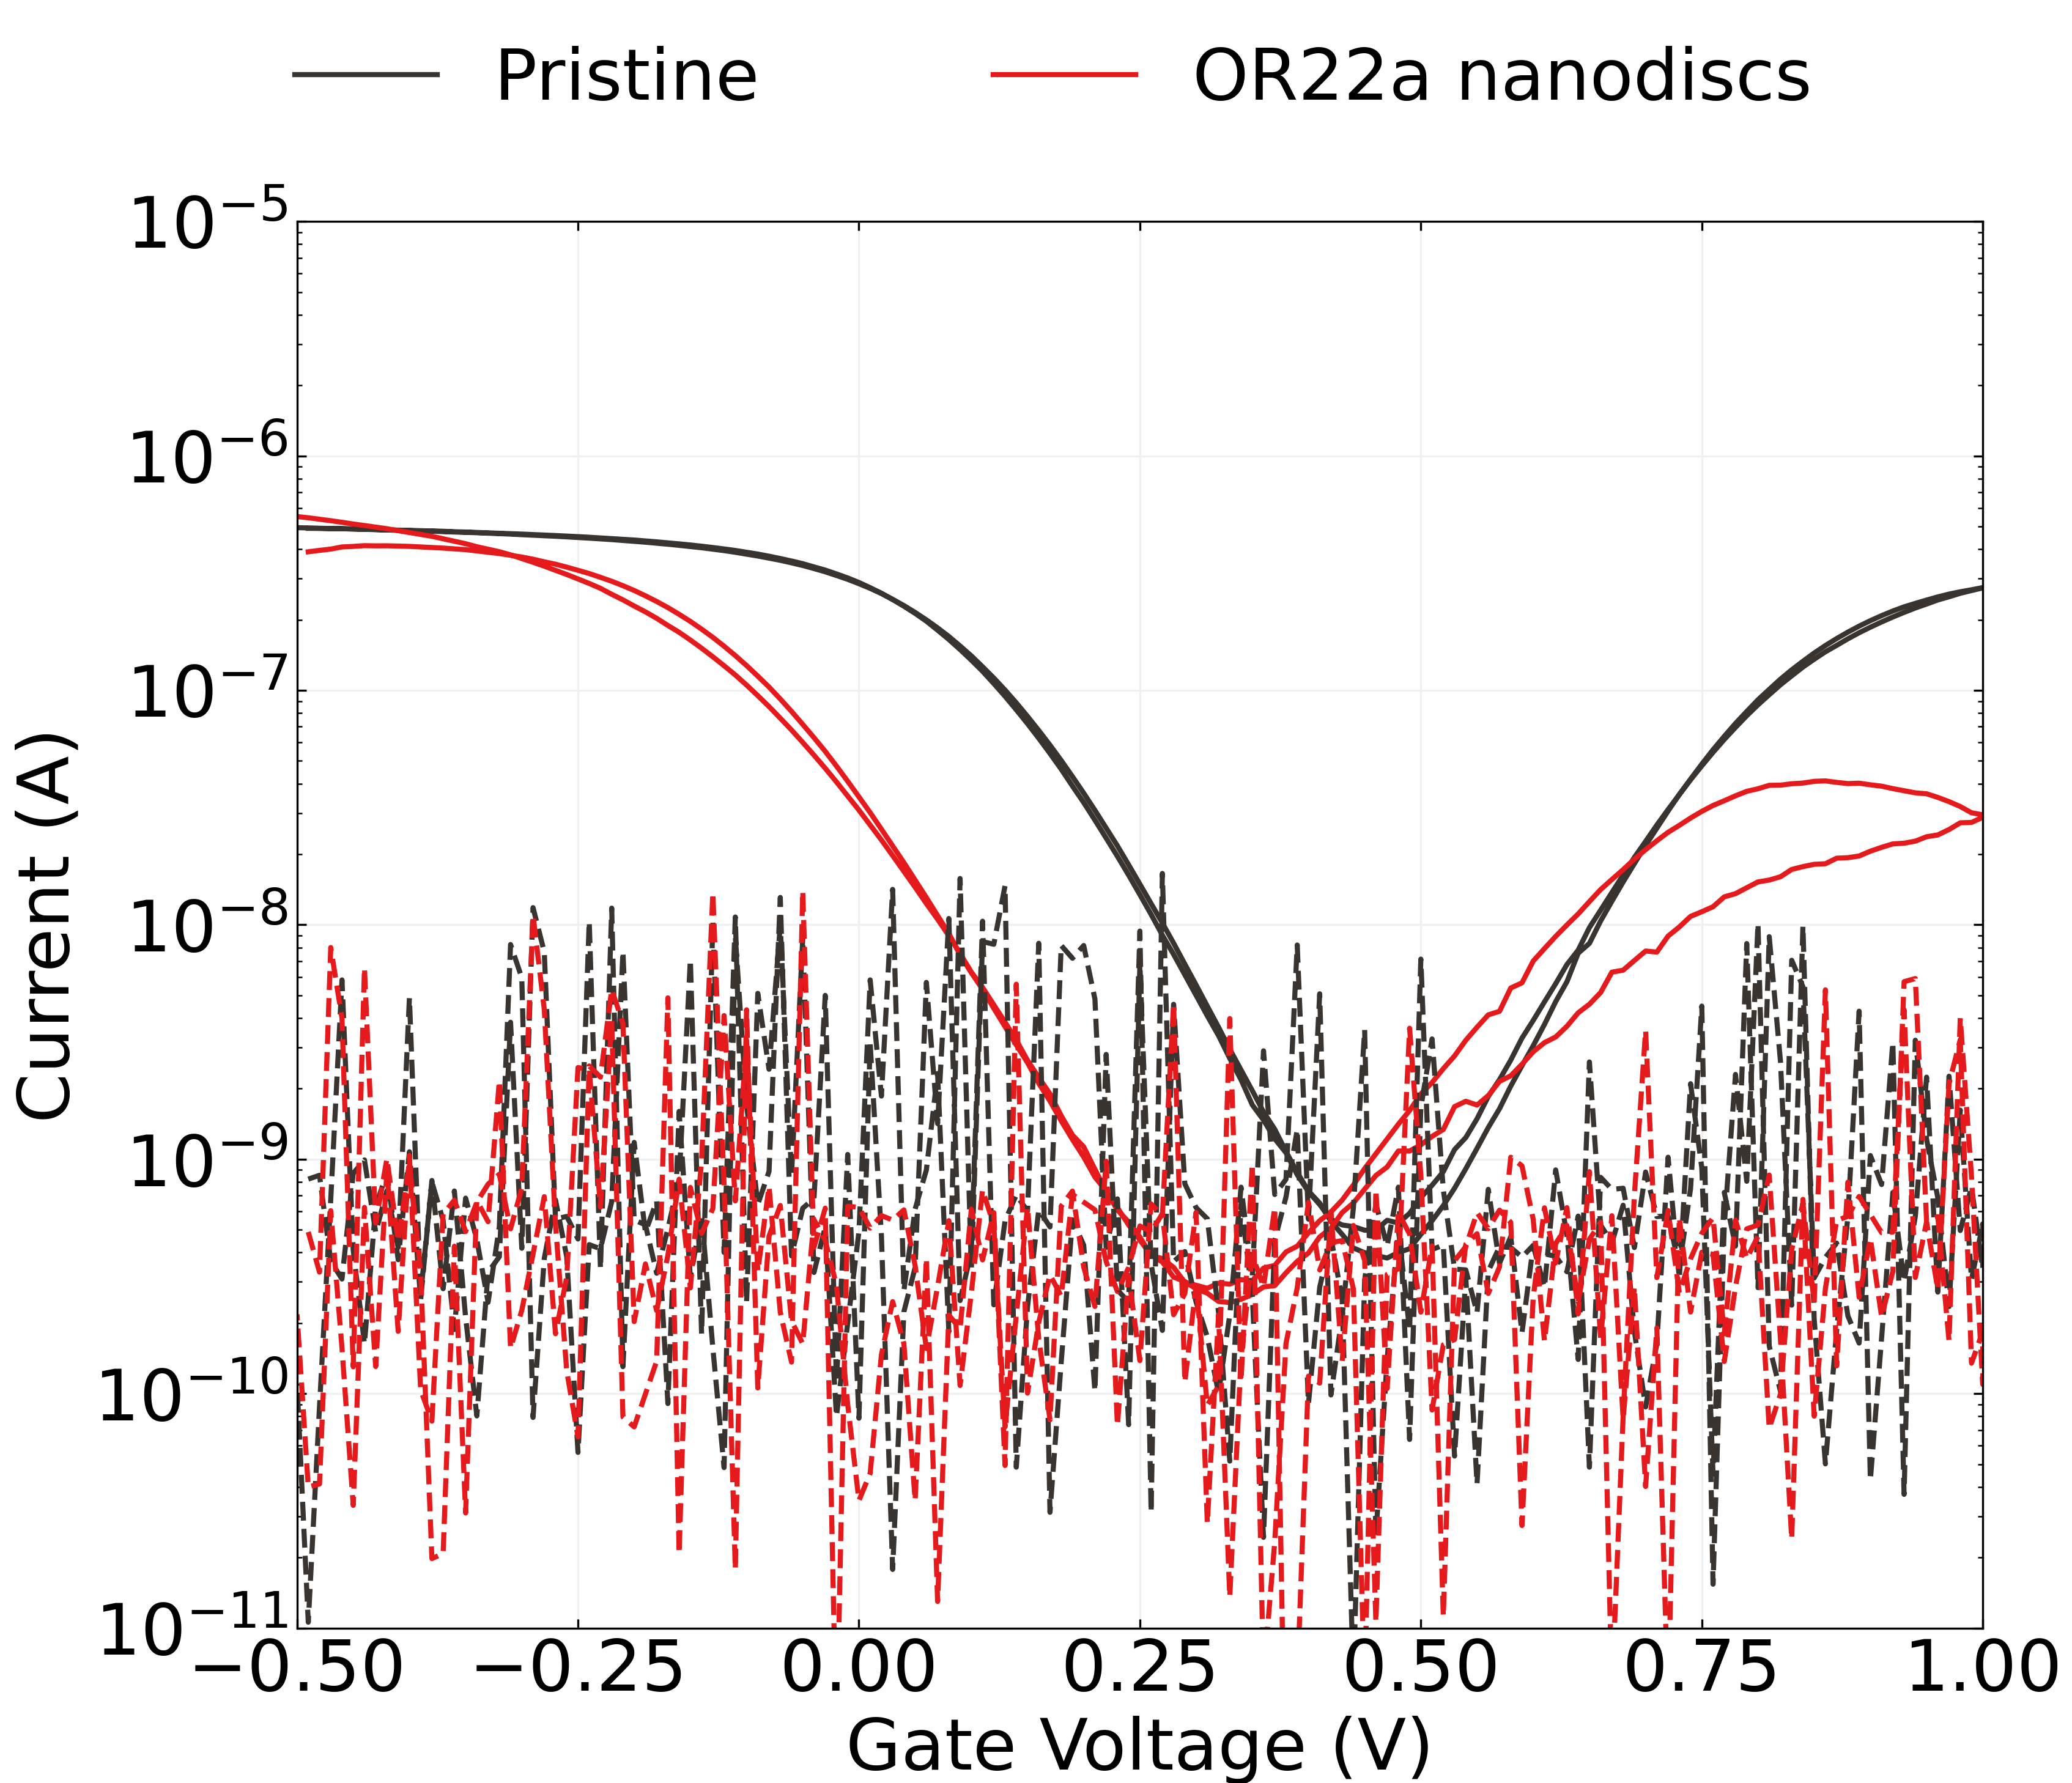
\includegraphics{figures/ch7/Q1C6_ch7_absolute_values_with_gate_current.png}

}

}

\end{minipage}%
%
\begin{minipage}[t]{0.01\linewidth}

{\centering 

~

}

\end{minipage}%
%
\begin{minipage}[t]{0.03\linewidth}

{\centering 

\raisebox{-\height}{


\includegraphics{figures/(b).png}

}

}

\end{minipage}%
%
\begin{minipage}[t]{0.01\linewidth}

{\centering 

~

}

\end{minipage}%
%
\begin{minipage}[t]{0.45\linewidth}

{\centering 

\raisebox{-\height}{

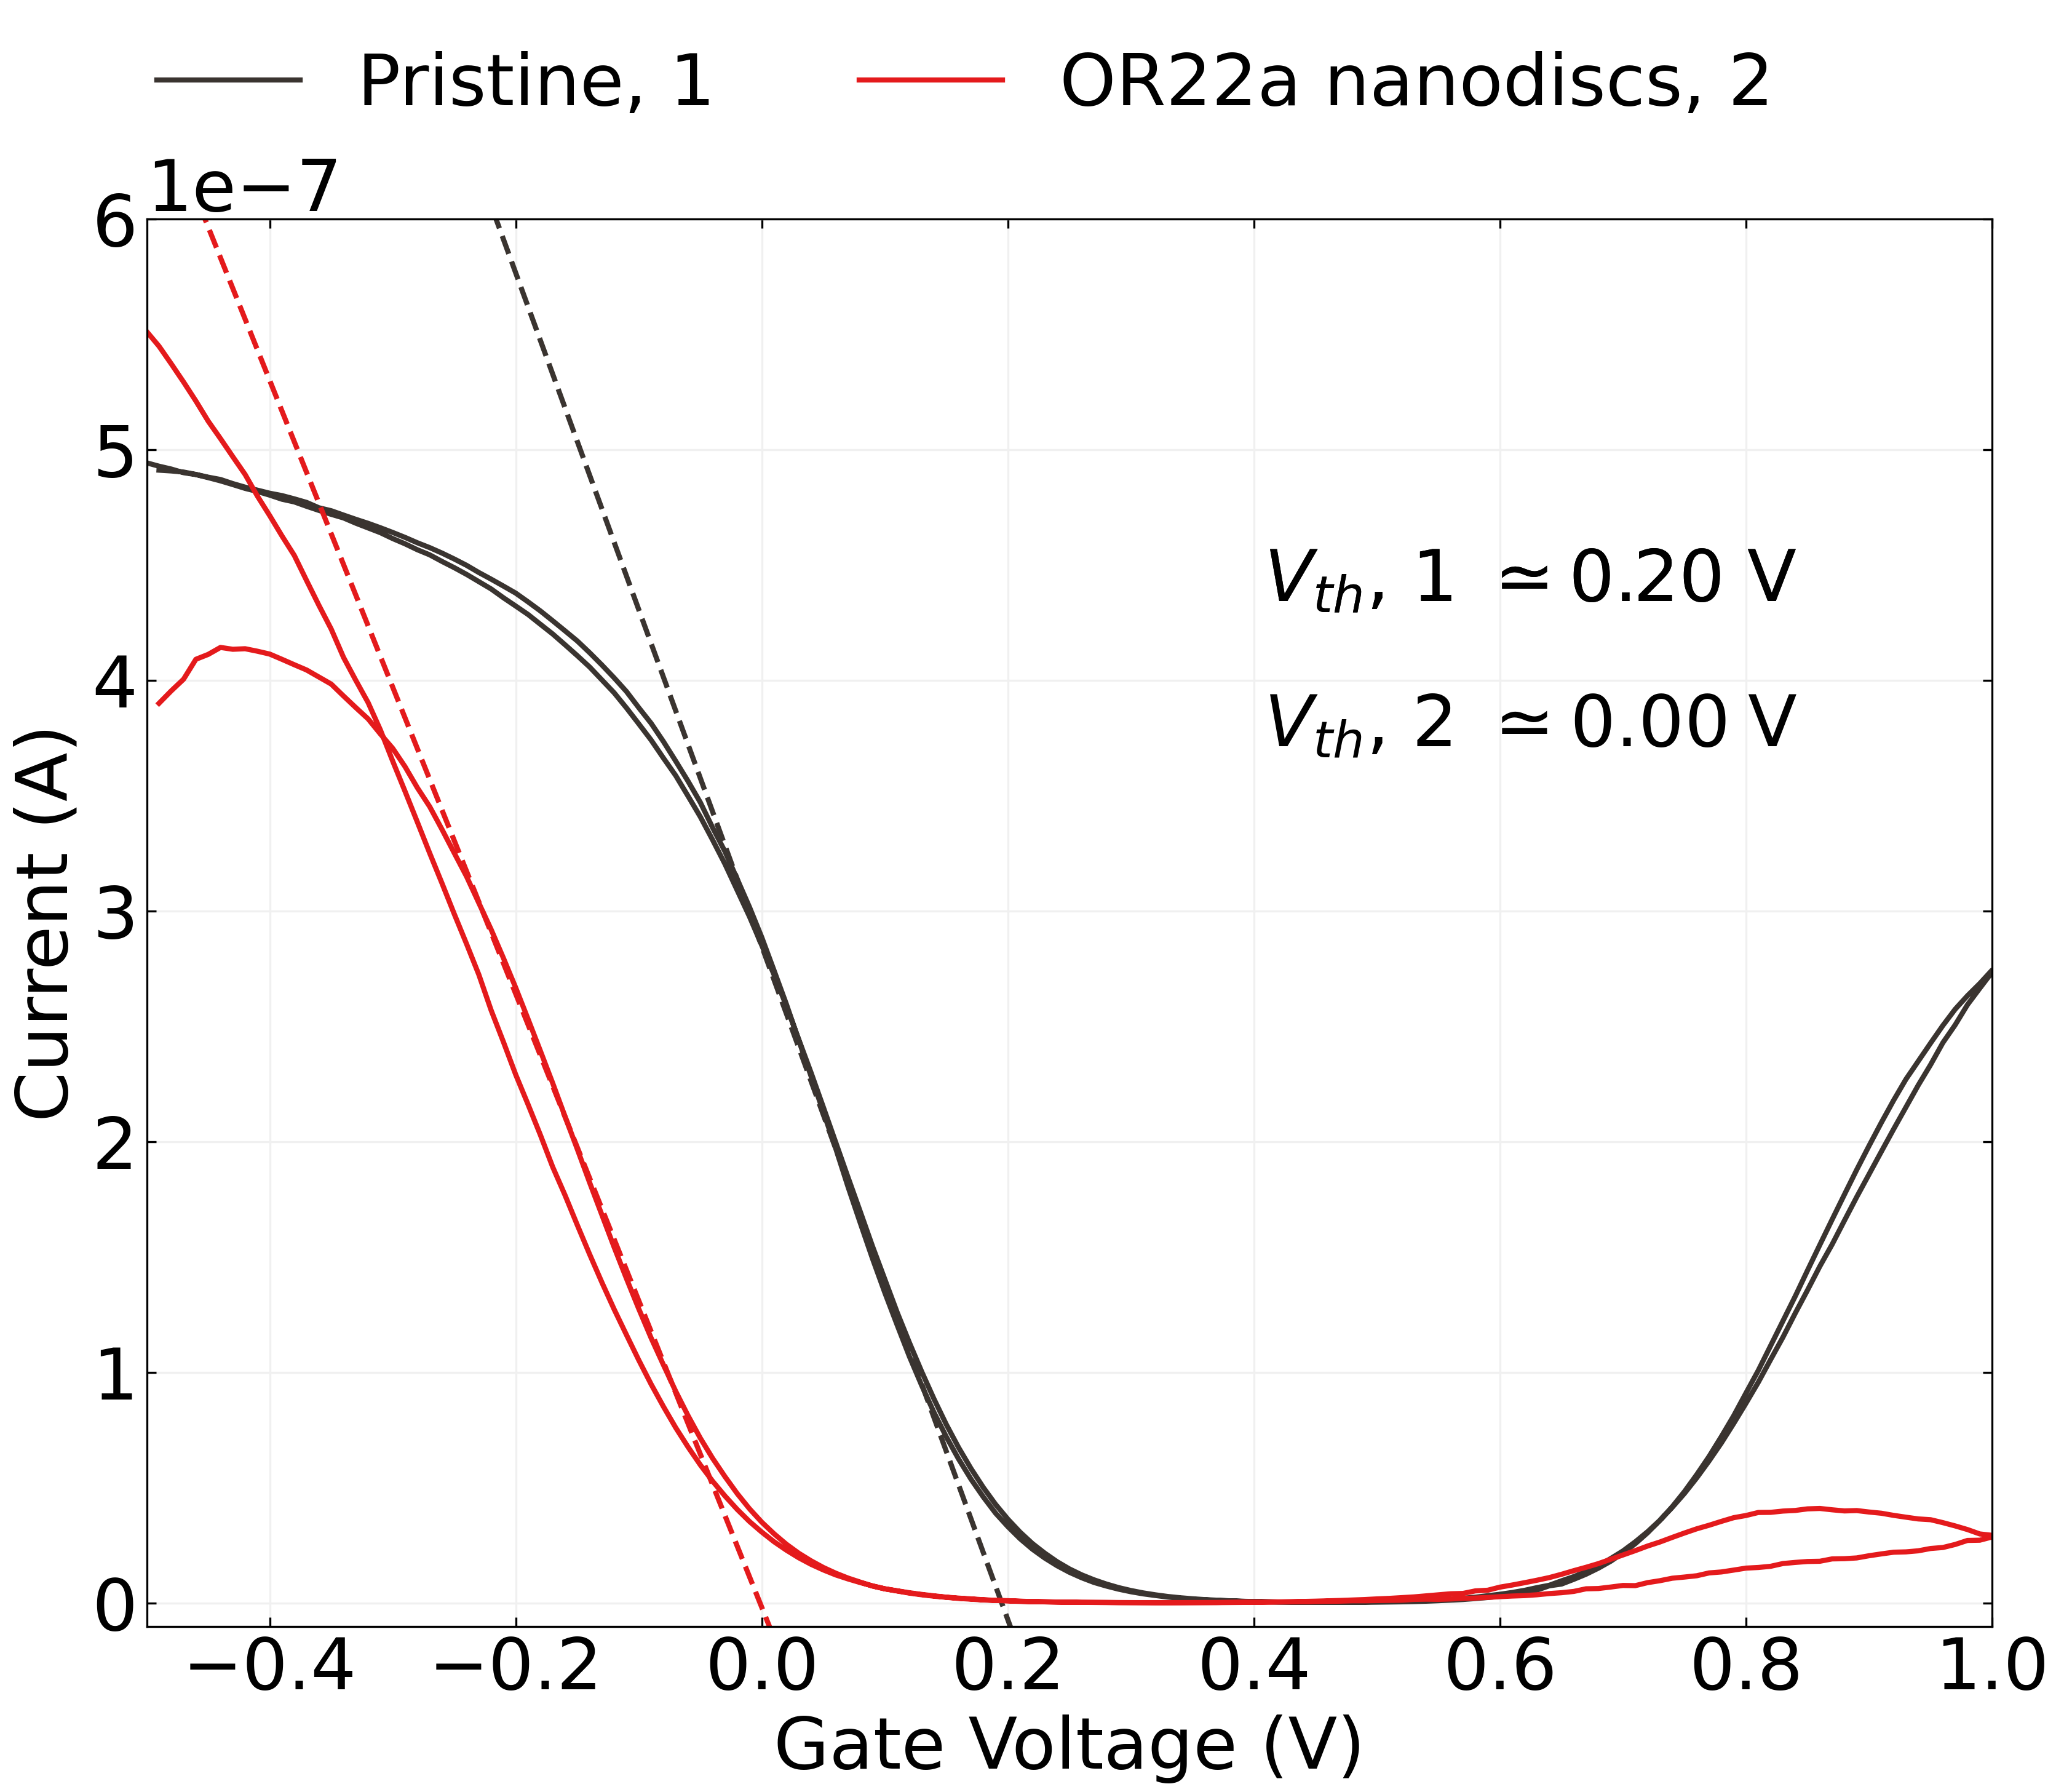
\includegraphics{figures/ch7/Q1C6_ch7_absolute_values_with_threshold_voltage_shift_without_gate_current.png}

}

}

\end{minipage}%
%
\begin{minipage}[t]{0.01\linewidth}

{\centering 

~

}

\end{minipage}%

\caption{\label{fig-OR22a-TX-comparison}Liquid-gated carbon nanotube
network device transfer characteristics before and after OR22a nanodisc
functionalisation. Source-drain voltage was \(V_{ds}\) = 100 mV for both
the forward and reverse sweep. In (a), the characteristics are shown on
a logarithmic scale, where the gate current for each transfer curve is
shown with a dashed line. In (b), the characteristics are shown on a
linear scale alongside a dashed line tangent to the subthreshold slope
of the characteristic curve in the forward direction. The threshold
voltage corresponding to the intercept of this slope with the x-axis is
shown for each transfer characteristic curve.}

\end{figure}

The liquid-gated electrical characteristics shown in
Figure~\ref{fig-OR22a-TX-comparison} were taken using the B1500A
semiconductor device analyser of the sensing channel (channel 7) before
and after functionalisation with OR22a nanodiscs. The liquid-gate
electrolyte used was \(1 \times\) PBS containing 0.5\% v/v DMSO. The
device exhibited ambipolar characteristics before functionalisation,
which is typically seen for steam-deposited carbon nanotube films
(\textbf{?@sec-electrical-characterisation-CNT};
\textbf{?@sec-cnt-devices}). However, \(p\)-type behaviour dominates
after device functionalisation due to a significant drop in \(n\)-type
conductance. A slight increase in hysteresis was observed
post-functionalisation. Leakage current (shown by the dashed traces)
never exceeded \(1 \times 10^{-7}\) V, both before and after
functionalisation. The significant change in electrical characteristics
could be due to some combination of five possible factors: adsorption of
solvent onto the network, network attachment of PBASE without subsequent
protein attachment, non-specific adsorption of protein onto the network,
PBASE-mediated attachment of the membrane scaffold protein (MSP) of
nanodiscs to the network, and PBASE-mediated attachment of odorant
receptors to the network. As the nanodisc volume is much larger than
that of the odorant receptor, any direct protein adsorption most likely
adsorption of the nanodisc membrane onto the carbon nanotube network.
Odorant receptor attachment with PBASE is therefore the only desirable
functionalisation result for sensing purposes.

Functionalisation of the channel resulted in a negative shift in
threshold voltage of \(-0.20 \pm 0.03\) V. This significantly exceeds
the threshold voltage shifts measured for both methanol adsorption
(\(-0.15 \pm 0.02\) V) and device exposure to PBASE in methanol
(\(-0.06 \pm 0.04\) V), confirming that protein has attached to the
carbon nanotubes. However, both direct protein adsorption
\autocite{Bradley2004,Heller2008,Kauffman2008} and empty nanodisc
membrane attachment \autocite{Murugathas2019a} should also lead to a
significant negative threshold voltage shift and therefore increased
\(p\)-conduction in the liquid-gated transfer characteristic curve. In
all three cases, the voltage shift is predominantly the result of
negative charge transfer from the adsorbed proteins to the
semiconducting carbon nanotubes
\autocite{Bradley2004,Heller2008,Murugathas2019a}. It is likely that the
negative shift observed results from some combination of the three types
of attachment. It should be noted that while the size of the
functionalisation-induced threshold voltage shift can be used to
determine whether an amine-tagged protein has attached to the nanodisc
network, it cannot be used to specifically determine whether odorant
receptors have attached to the network.

Atomic force microscope images were taken of the device channels both
before functionalisation and after sensing with the functionalised
device to confirm the presence of nanodiscs. The images are shown in
Figure~\ref{fig-working-OR22a-AFM} (a)-(b). As far as the author knows,
these are the first atomic force microscope images taken of iOR
nanodiscs found on a sensing channel rather than on a separate carbon
nanotube film; this was made possible by using the 20 µm wide aperture
encapsulation mask discussed in \textbf{?@sec-encapsulation}. AFM images
showing iOR-nanodisc functionalised carbon nanotube networks have been
reported by Murugathas \emph{et al.}, but these images were not of
channels used for sensing \autocite{Murugathas2019a}. The visible
nanodisc features in Figure~\ref{fig-working-OR22a-AFM} (b) are much
smaller than the aggregated or agglomerated nanodisc features in the
atomic microscope images taken by Murugathas \emph{et al.}
\autocite{Murugathas2019a}. On the dense network morphology used here,
the position of nanodisc clusters relative to the carbon nanotubes is
also less distinct. To confirm whether nanodiscs have preferentially
attached to the carbon nanotubes, a more quantitative approach is
required.

\begin{figure}

\begin{minipage}[t]{0.03\linewidth}

{\centering 

\raisebox{-\height}{


\includegraphics{figures/(a).png}

}

}

\end{minipage}%
%
\begin{minipage}[t]{0.01\linewidth}

{\centering 

~

}

\end{minipage}%
%
\begin{minipage}[t]{0.45\linewidth}

{\centering 

\raisebox{-\height}{

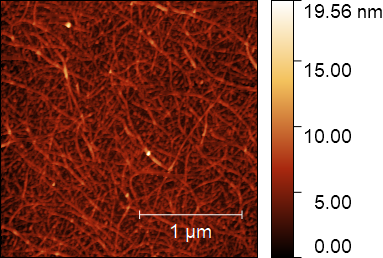
\includegraphics{figures/ch7/Pristine_DF2Q3D10_00141.png}

}

}

\end{minipage}%
%
\begin{minipage}[t]{0.01\linewidth}

{\centering 

~

}

\end{minipage}%
%
\begin{minipage}[t]{0.03\linewidth}

{\centering 

\raisebox{-\height}{


\includegraphics{figures/(b).png}

}

}

\end{minipage}%
%
\begin{minipage}[t]{0.01\linewidth}

{\centering 

~

}

\end{minipage}%
%
\begin{minipage}[t]{0.45\linewidth}

{\centering 

\raisebox{-\height}{

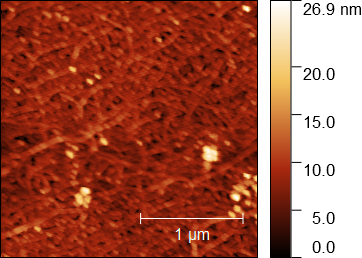
\includegraphics{figures/ch7/DF2Q1D6_postNDOR22a_ch7_1_00375.png}

}

}

\end{minipage}%
%
\begin{minipage}[t]{0.01\linewidth}

{\centering 

~

}

\end{minipage}%
\newline
\begin{minipage}[t]{0.03\linewidth}

{\centering 

\raisebox{-\height}{


\includegraphics{figures/(c).png}

}

}

\end{minipage}%
%
\begin{minipage}[t]{0.01\linewidth}

{\centering 

~

}

\end{minipage}%
%
\begin{minipage}[t]{0.45\linewidth}

{\centering 

\raisebox{-\height}{

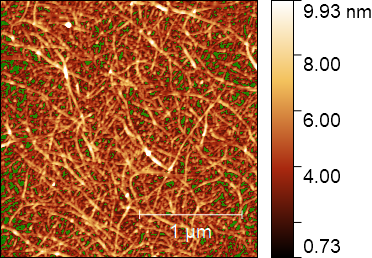
\includegraphics{figures/ch7/Pristine_DF2Q3D10_00141_mask.png}

}

}

\end{minipage}%
%
\begin{minipage}[t]{0.01\linewidth}

{\centering 

~

}

\end{minipage}%
%
\begin{minipage}[t]{0.03\linewidth}

{\centering 

\raisebox{-\height}{


\includegraphics{figures/(d).png}

}

}

\end{minipage}%
%
\begin{minipage}[t]{0.01\linewidth}

{\centering 

~

}

\end{minipage}%
%
\begin{minipage}[t]{0.45\linewidth}

{\centering 

\raisebox{-\height}{

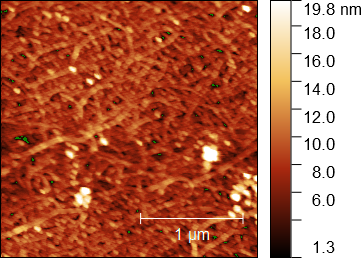
\includegraphics{figures/ch7/DF2Q1D6_postNDOR22a_ch7_1_00375_mask.png}

}

}

\end{minipage}%
%
\begin{minipage}[t]{0.01\linewidth}

{\centering 

~

}

\end{minipage}%
\newline
\begin{minipage}[t]{0.03\linewidth}

{\centering 

\raisebox{-\height}{


\includegraphics{figures/(e).png}

}

}

\end{minipage}%
%
\begin{minipage}[t]{0.01\linewidth}

{\centering 

~

}

\end{minipage}%
%
\begin{minipage}[t]{0.45\linewidth}

{\centering 

\raisebox{-\height}{

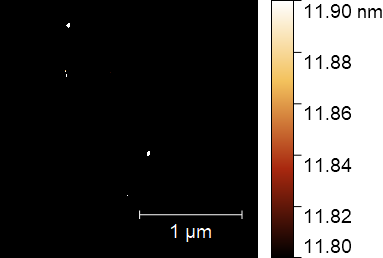
\includegraphics{figures/ch7/Pristine_DF2Q3D10_00141_crosssection.png}

}

}

\end{minipage}%
%
\begin{minipage}[t]{0.01\linewidth}

{\centering 

~

}

\end{minipage}%
%
\begin{minipage}[t]{0.03\linewidth}

{\centering 

\raisebox{-\height}{


\includegraphics{figures/(f).png}

}

}

\end{minipage}%
%
\begin{minipage}[t]{0.01\linewidth}

{\centering 

~

}

\end{minipage}%
%
\begin{minipage}[t]{0.45\linewidth}

{\centering 

\raisebox{-\height}{

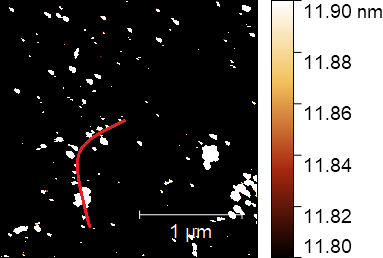
\includegraphics{figures/ch7/DF2Q1D6_postNDOR22a_ch7_1_00375_crosssection_edit.png}

}

}

\end{minipage}%
%
\begin{minipage}[t]{0.01\linewidth}

{\centering 

~

}

\end{minipage}%

\caption{\label{fig-working-OR22a-AFM}Atomic force microscope images of
the channel region of carbon nanotube network devices before and after
functionalisation. The channel network of a pristine device is shown in
(a), while (b) is of channel 7 from the sensing device functionalised in
this section. The same images over a smaller height scale are shown in
(c) and (d), with regions at or below the median substrate height (2 nm)
highlighted green. Binary representations of the atomic force microscope
images are shown in (e) for the the pristine device and (f) for the
functionalised device, with a threshold height of 12 nm used (10 nm
above the average substrate height).}

\end{figure}

Following the discussion in \textbf{?@sec-pristine-AFM}, the median
substrate height in Figure~\ref{fig-working-OR22a-AFM} (b) is assumed to
be \(\sim\) 2 nm as there are no visible imaging artifacts. This height
is shown against each carbon nanotube network using the Gwyddion masking
tool in Figure~\ref{fig-working-OR22a-AFM} (c) and (d). In Gwyddion,
both images were then simplified to a binary representation, where
features above a certain threshold were shown as white and features
below shown as black. This representation, shown in
Figure~\ref{fig-working-OR22a-AFM} (e) and (f), has the appearance of a
cross-section through the network at the threshold height. The threshold
was chosen as the minimum height where carbon nanotube spindles were no
longer apparent in the functionalised image, 10 nm above the substrate.
Figure~\ref{fig-working-OR22a-AFM} (e) shows only a few, sparsely
distributed features, each with a width below 50 nm. These features may
correspond to large nanotube-nanotube junctions, surfactant residue, or
other surface contamination (\textbf{?@sec-pristine-morphology}). In
Figure~\ref{fig-working-OR22a-AFM} (f), many features are over 50 nm in
width. They are often found close together, and form a curved line
across the network in the bottom left corner (shown in red); this
arrangement of nanodisc features is similar to that reported previously
for OR22a nanodiscs on sparser, more bundled networks
\autocite{Murugathas2019a}.

Figure~\ref{fig-working-OR22a-AFM} (b) shows that the maximum image
height of the OR nanodisc-functionalised channel is 27 nm, while
Figure~\ref{fig-working-OR22a-AFM} (f) indicates only nanodisc features
are present at 12 nm. Therefore, nanodisc agglomerates at least 15 nm
tall are present on the channel. Assuming a average carbon nanotube
bundle diameter of 2 nm, with an average substrate height of 2 nm, the
nanodisc agglomerates visible in Figure~\ref{fig-working-OR22a-AFM}
could be up to \(\sim\) 23 nm tall. The estimated height range for
nanodiscs is \(\sim 10 - 20\) nm
\autocite{Nath2007,Bayburt2010,Murugathas2020,Cheema2021}. It therefore
appears that nanodiscs have formed a single layer on the carbon nanotube
network. Height measurements of biological samples taken via AFM have
been shown to underestimate actual feature height by over 50\%
\autocite{Vobornik2023}. Even so \(-\) assuming this squishing effect is
not significantly in excess of 50\% \(-\) the agglomerates are only a
few nanodiscs high at most. As the nanodisc agglomerates are up to 200
nm across at their widest point (Figure~\ref{fig-working-OR22a-AFM}),
comprising of at least 20 nanodiscs, it appears that the clustering
behaviour is primarily across the plane rather than vertical. The
observed behaviour indicates nanodiscs individually attach to preferred
locations on the network instead of nucleating in solution prior to
attachment.

This attachment behaviour can be contrasted with the behaviour observed
in the atomic microscope image of agglomerated OR22a nanodiscs taken by
Murugathas \emph{et al.} \autocite{Murugathas2019a}. The network is
significantly sparser, so the relative extent of clustering at different
points is easier to discern. There is clearly significant variation in
nanodisc attachment across a single nanotube bundle, and it appears that
clustering is more significant at junctions between carbon nanotube
bundles. Preferred attachment locations away from junctions could result
from the higher reactivity of exposed metallic CNTs \autocite{Cao2009},
or from regions which are particularly clean of contamination.
Interestingly, while the OR22a nanodisc features seen by Murugathas
\emph{et al.} via AFM are similar in breadth to those seen here, OR
agglomerates which are at least 53 nm tall are present
\autocite{Murugathas2020}. It is unclear why the extent of vertical
agglomeration differs between this work and that of Murugathas \emph{et
al.}, but may be linked to the difference in morphology between the
networks used. One possibility is that nanodiscs will preferentially
attach to metallic carbon nanotubes, but prefer to attach to each other
instead of semiconducting nanotubes. Semiconducting tubes in a highly
bundled network may block proteins from accessing metallic tubes in the
same bundle, leading to a greater degree of self-attachment.

\begin{figure}

\begin{minipage}[t]{0.03\linewidth}

{\centering 

\raisebox{-\height}{


\includegraphics{figures/(a).png}

}

}

\end{minipage}%
%
\begin{minipage}[t]{0.01\linewidth}

{\centering 

~

}

\end{minipage}%
%
\begin{minipage}[t]{0.45\linewidth}

{\centering 

\raisebox{-\height}{

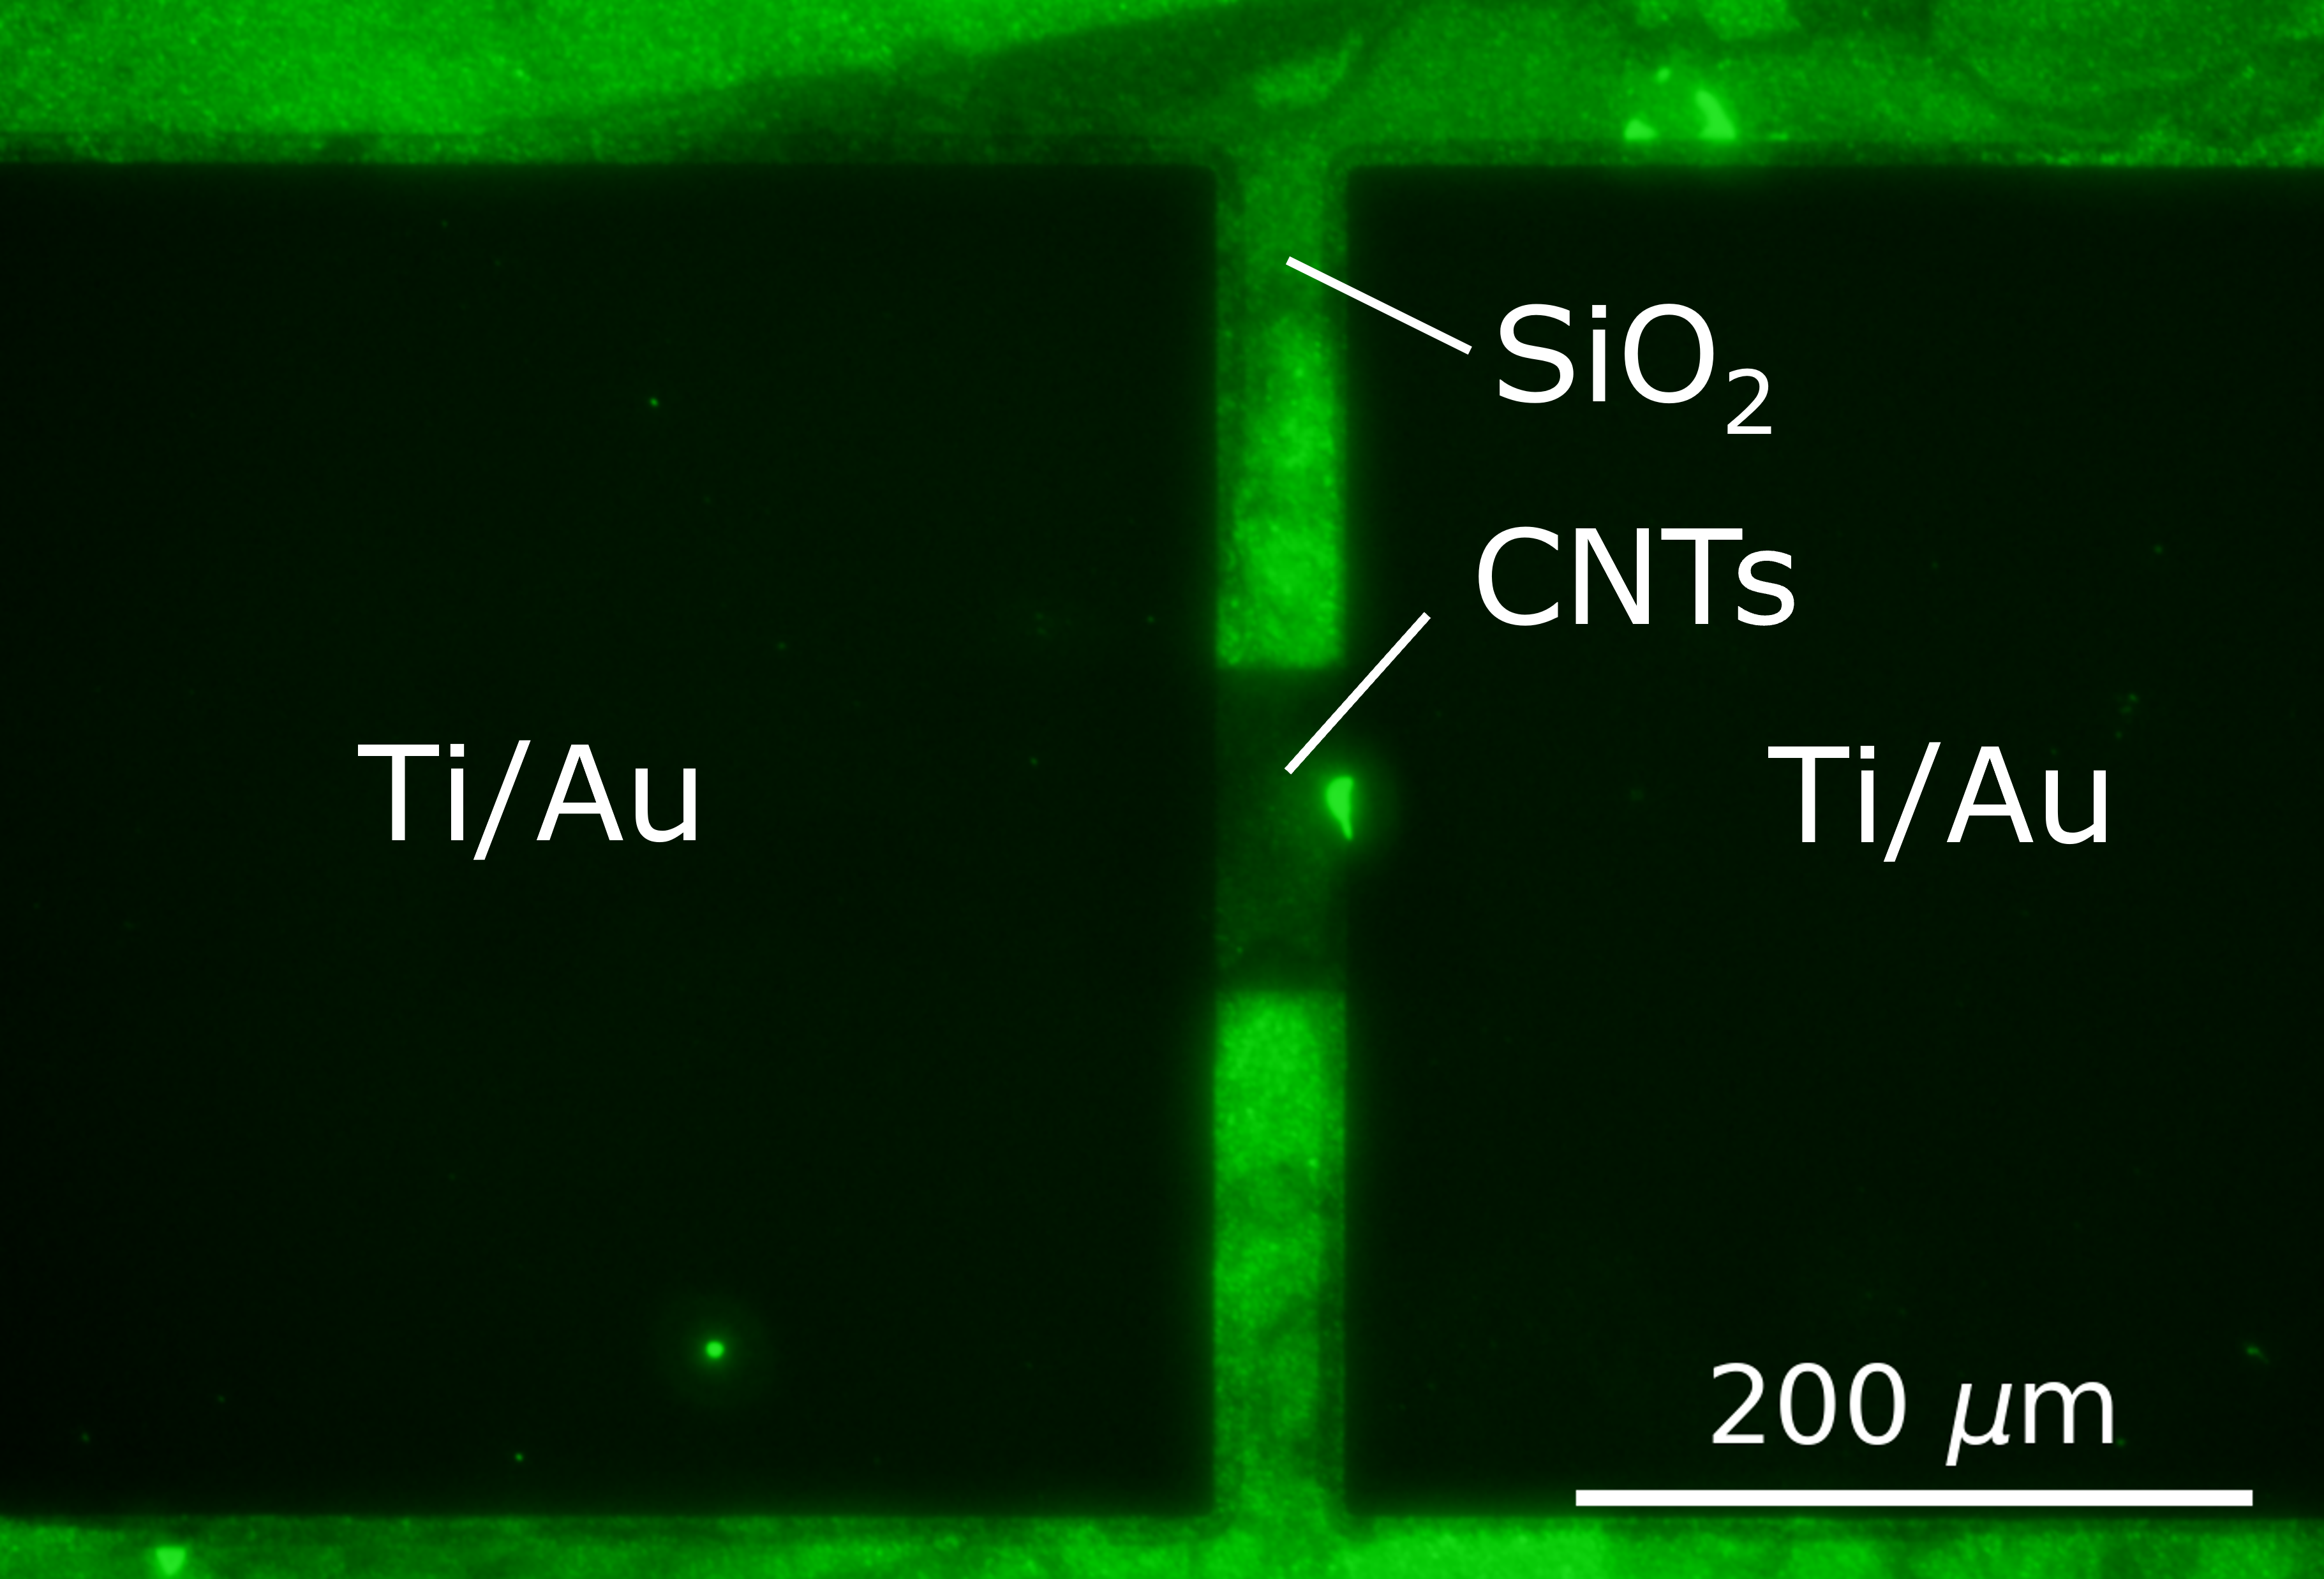
\includegraphics{figures/ch7/modified_GFPOR_10sexposure_20X_mediumcontrast_ch6_240208.png}

}

}

\end{minipage}%
%
\begin{minipage}[t]{0.01\linewidth}

{\centering 

~

}

\end{minipage}%
%
\begin{minipage}[t]{0.03\linewidth}

{\centering 

\raisebox{-\height}{


\includegraphics{figures/(b).png}

}

}

\end{minipage}%
%
\begin{minipage}[t]{0.01\linewidth}

{\centering 

~

}

\end{minipage}%
%
\begin{minipage}[t]{0.45\linewidth}

{\centering 

\raisebox{-\height}{

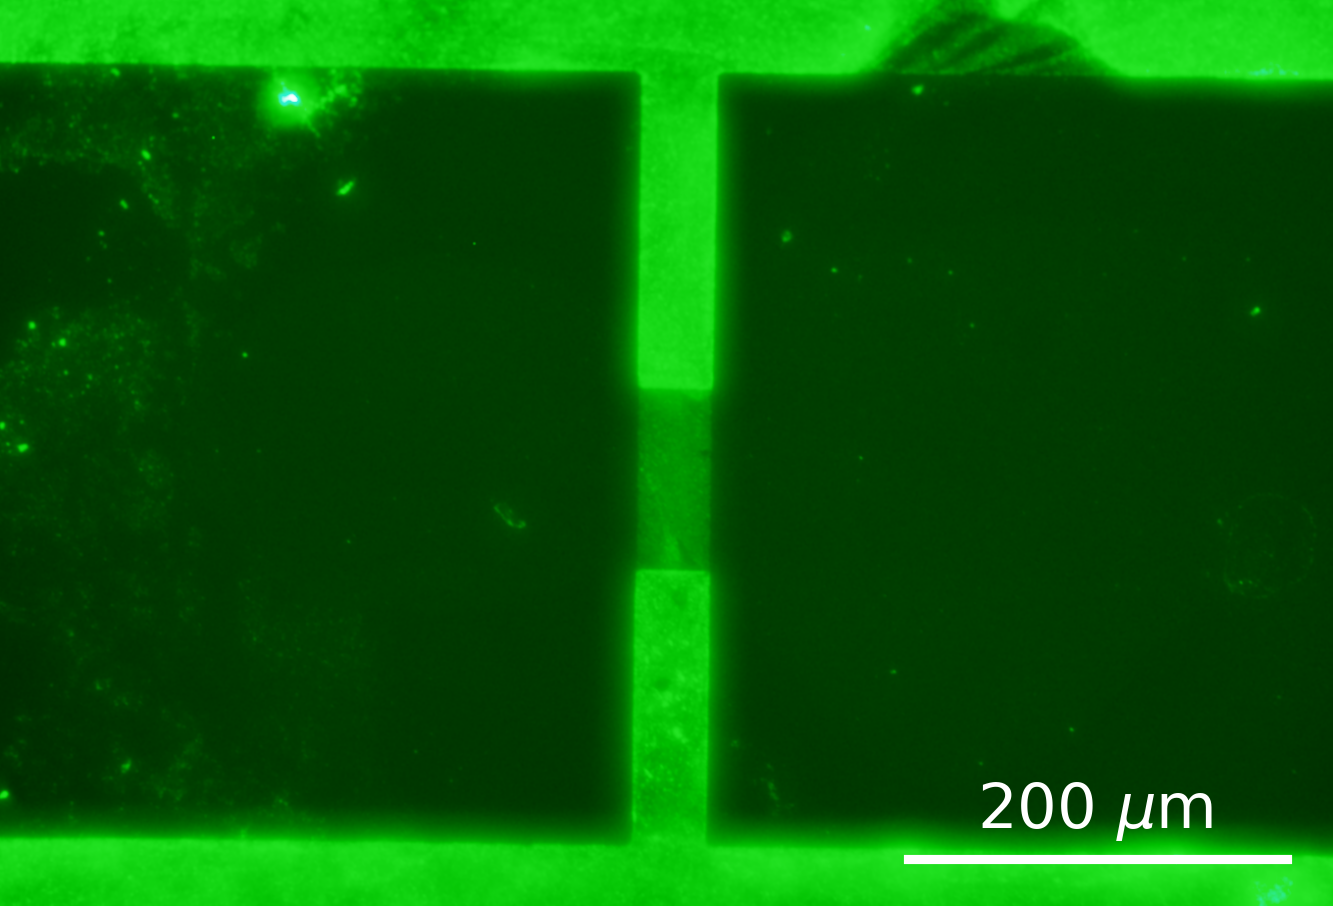
\includegraphics{figures/ch7/modified_GFPOR_PBASE_10sexposure_20X_mediumcontrast_ch1_231019_2.png}

}

}

\end{minipage}%
%
\begin{minipage}[t]{0.01\linewidth}

{\centering 

~

}

\end{minipage}%
\newline
\begin{minipage}[t]{0.03\linewidth}

{\centering 

\raisebox{-\height}{


\includegraphics{figures/(c).png}

}

}

\end{minipage}%
%
\begin{minipage}[t]{0.01\linewidth}

{\centering 

~

}

\end{minipage}%
%
\begin{minipage}[t]{0.45\linewidth}

{\centering 

\raisebox{-\height}{

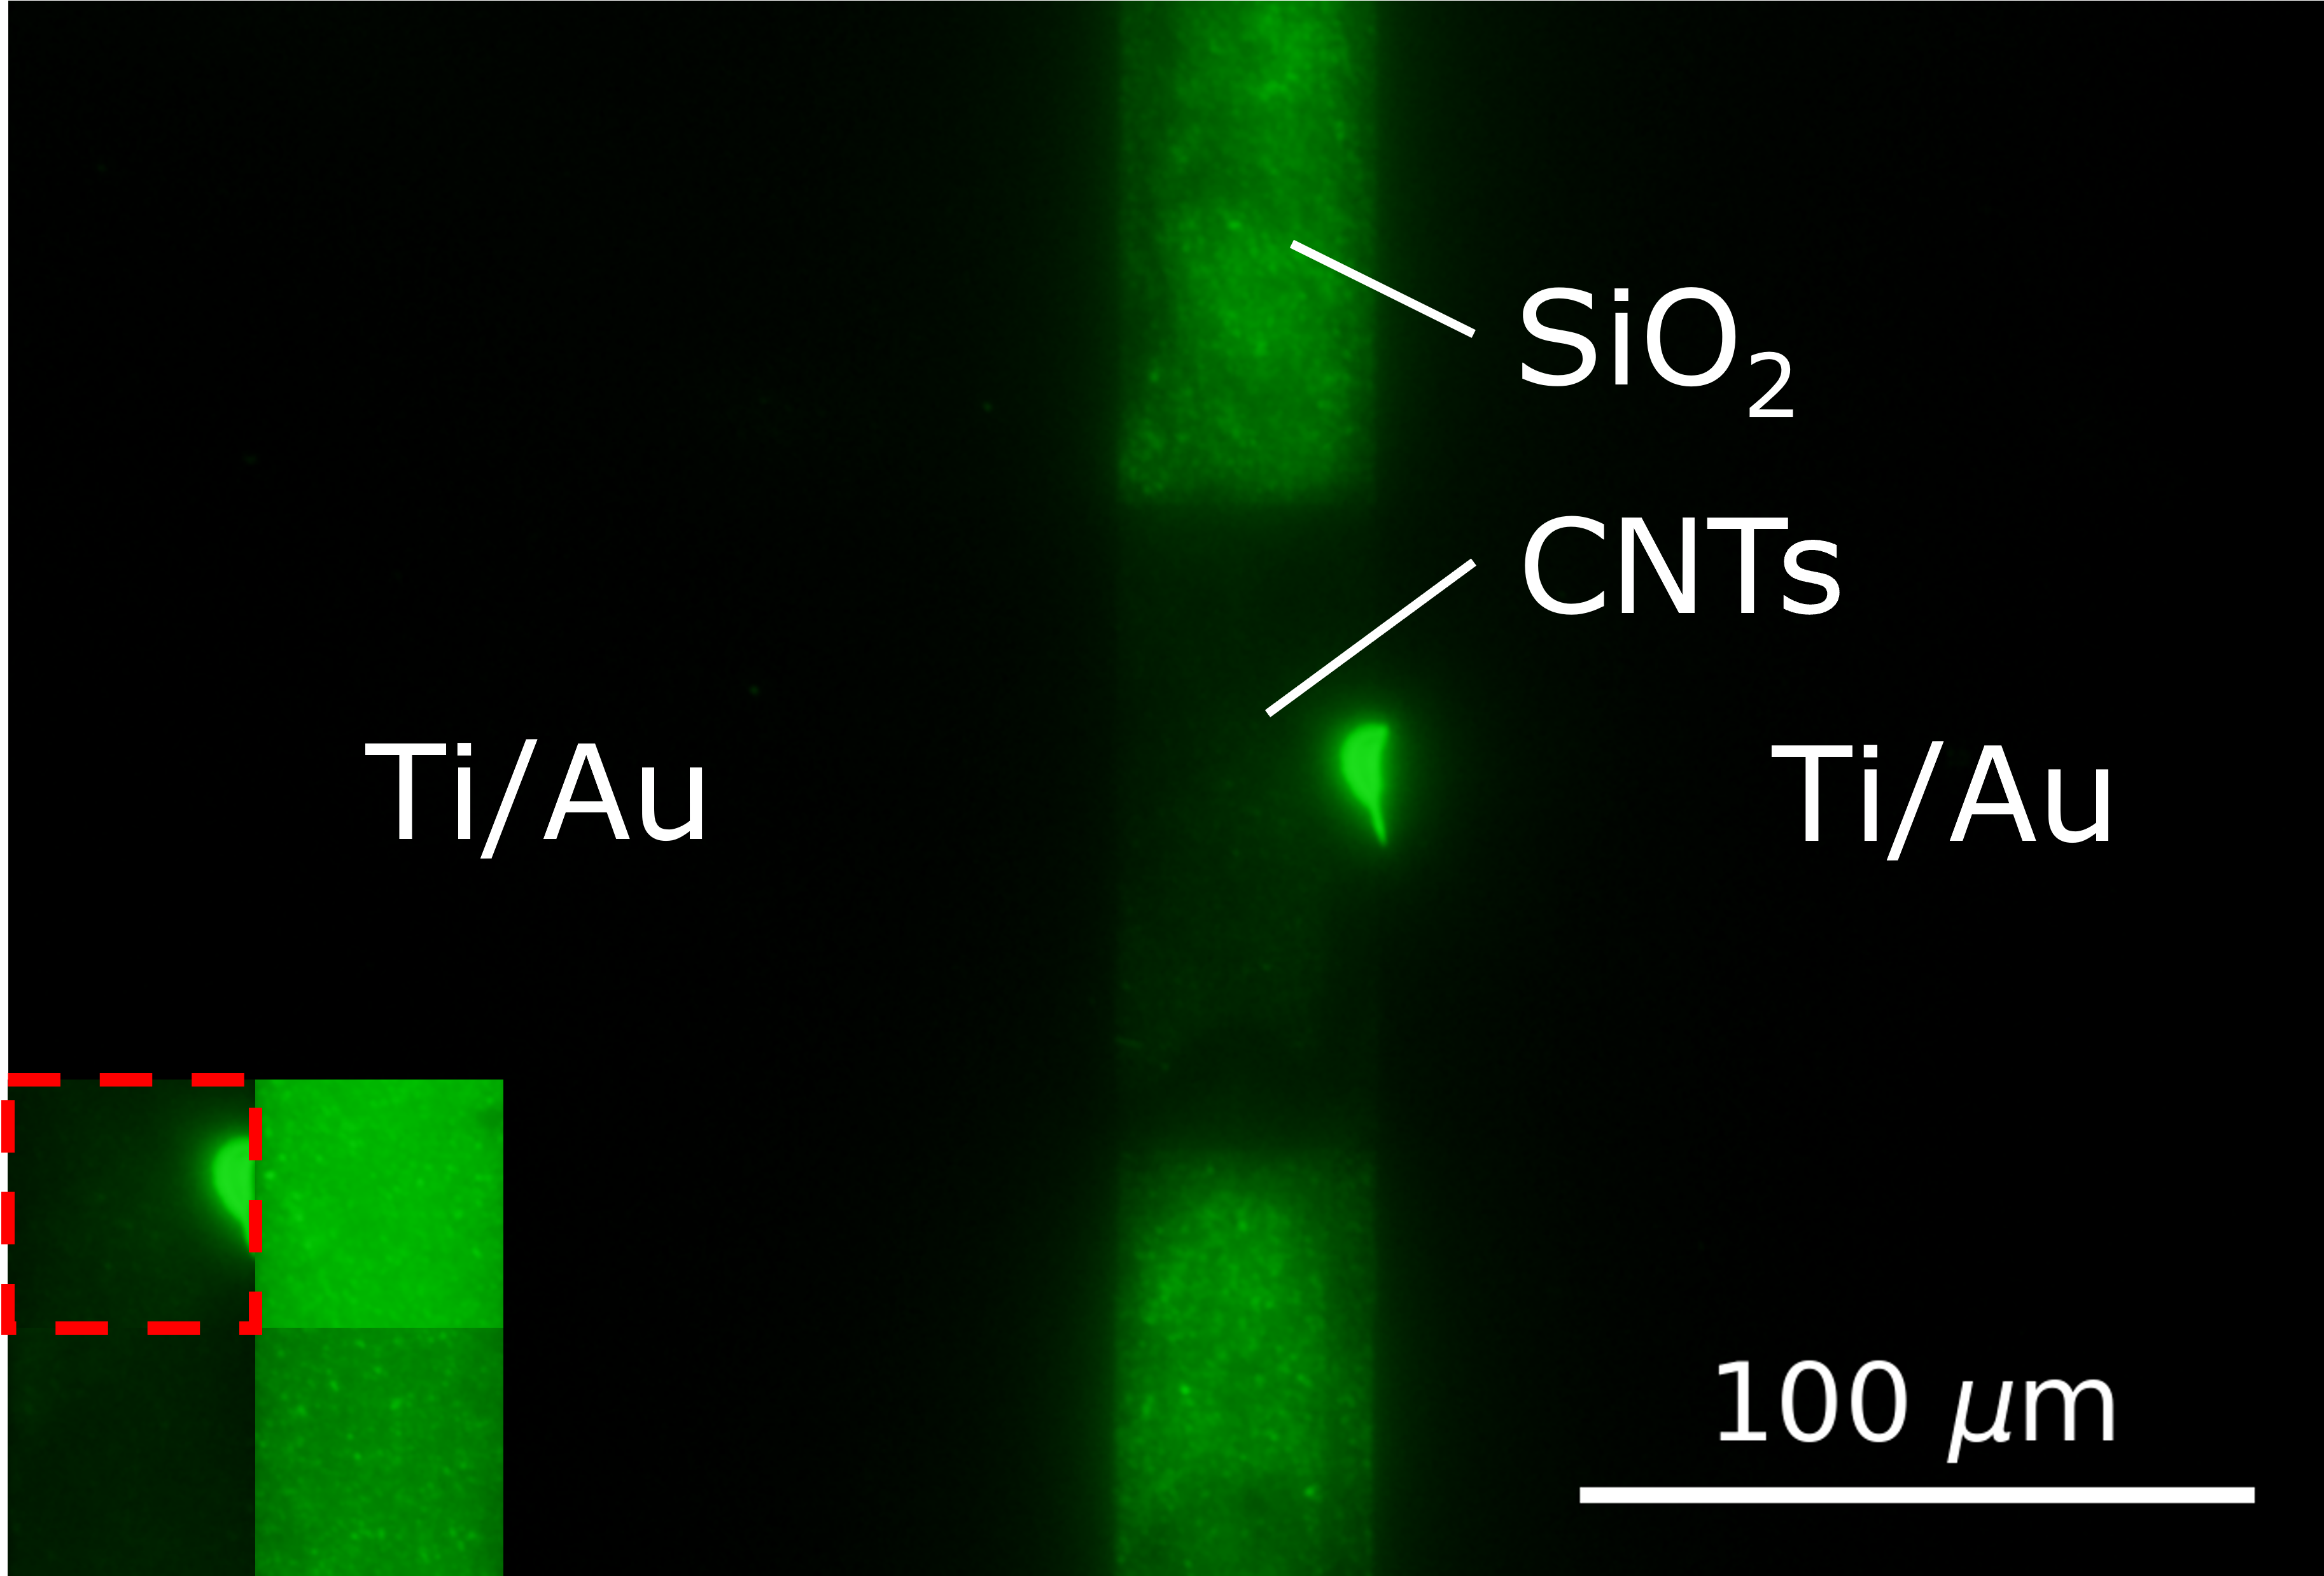
\includegraphics{figures/ch7/modified_GFPOR_10sexposure_40X_mediumcontrast_ch6_240208.png}

}

}

\end{minipage}%
%
\begin{minipage}[t]{0.01\linewidth}

{\centering 

~

}

\end{minipage}%
%
\begin{minipage}[t]{0.03\linewidth}

{\centering 

\raisebox{-\height}{


\includegraphics{figures/(d).png}

}

}

\end{minipage}%
%
\begin{minipage}[t]{0.01\linewidth}

{\centering 

~

}

\end{minipage}%
%
\begin{minipage}[t]{0.45\linewidth}

{\centering 

\raisebox{-\height}{

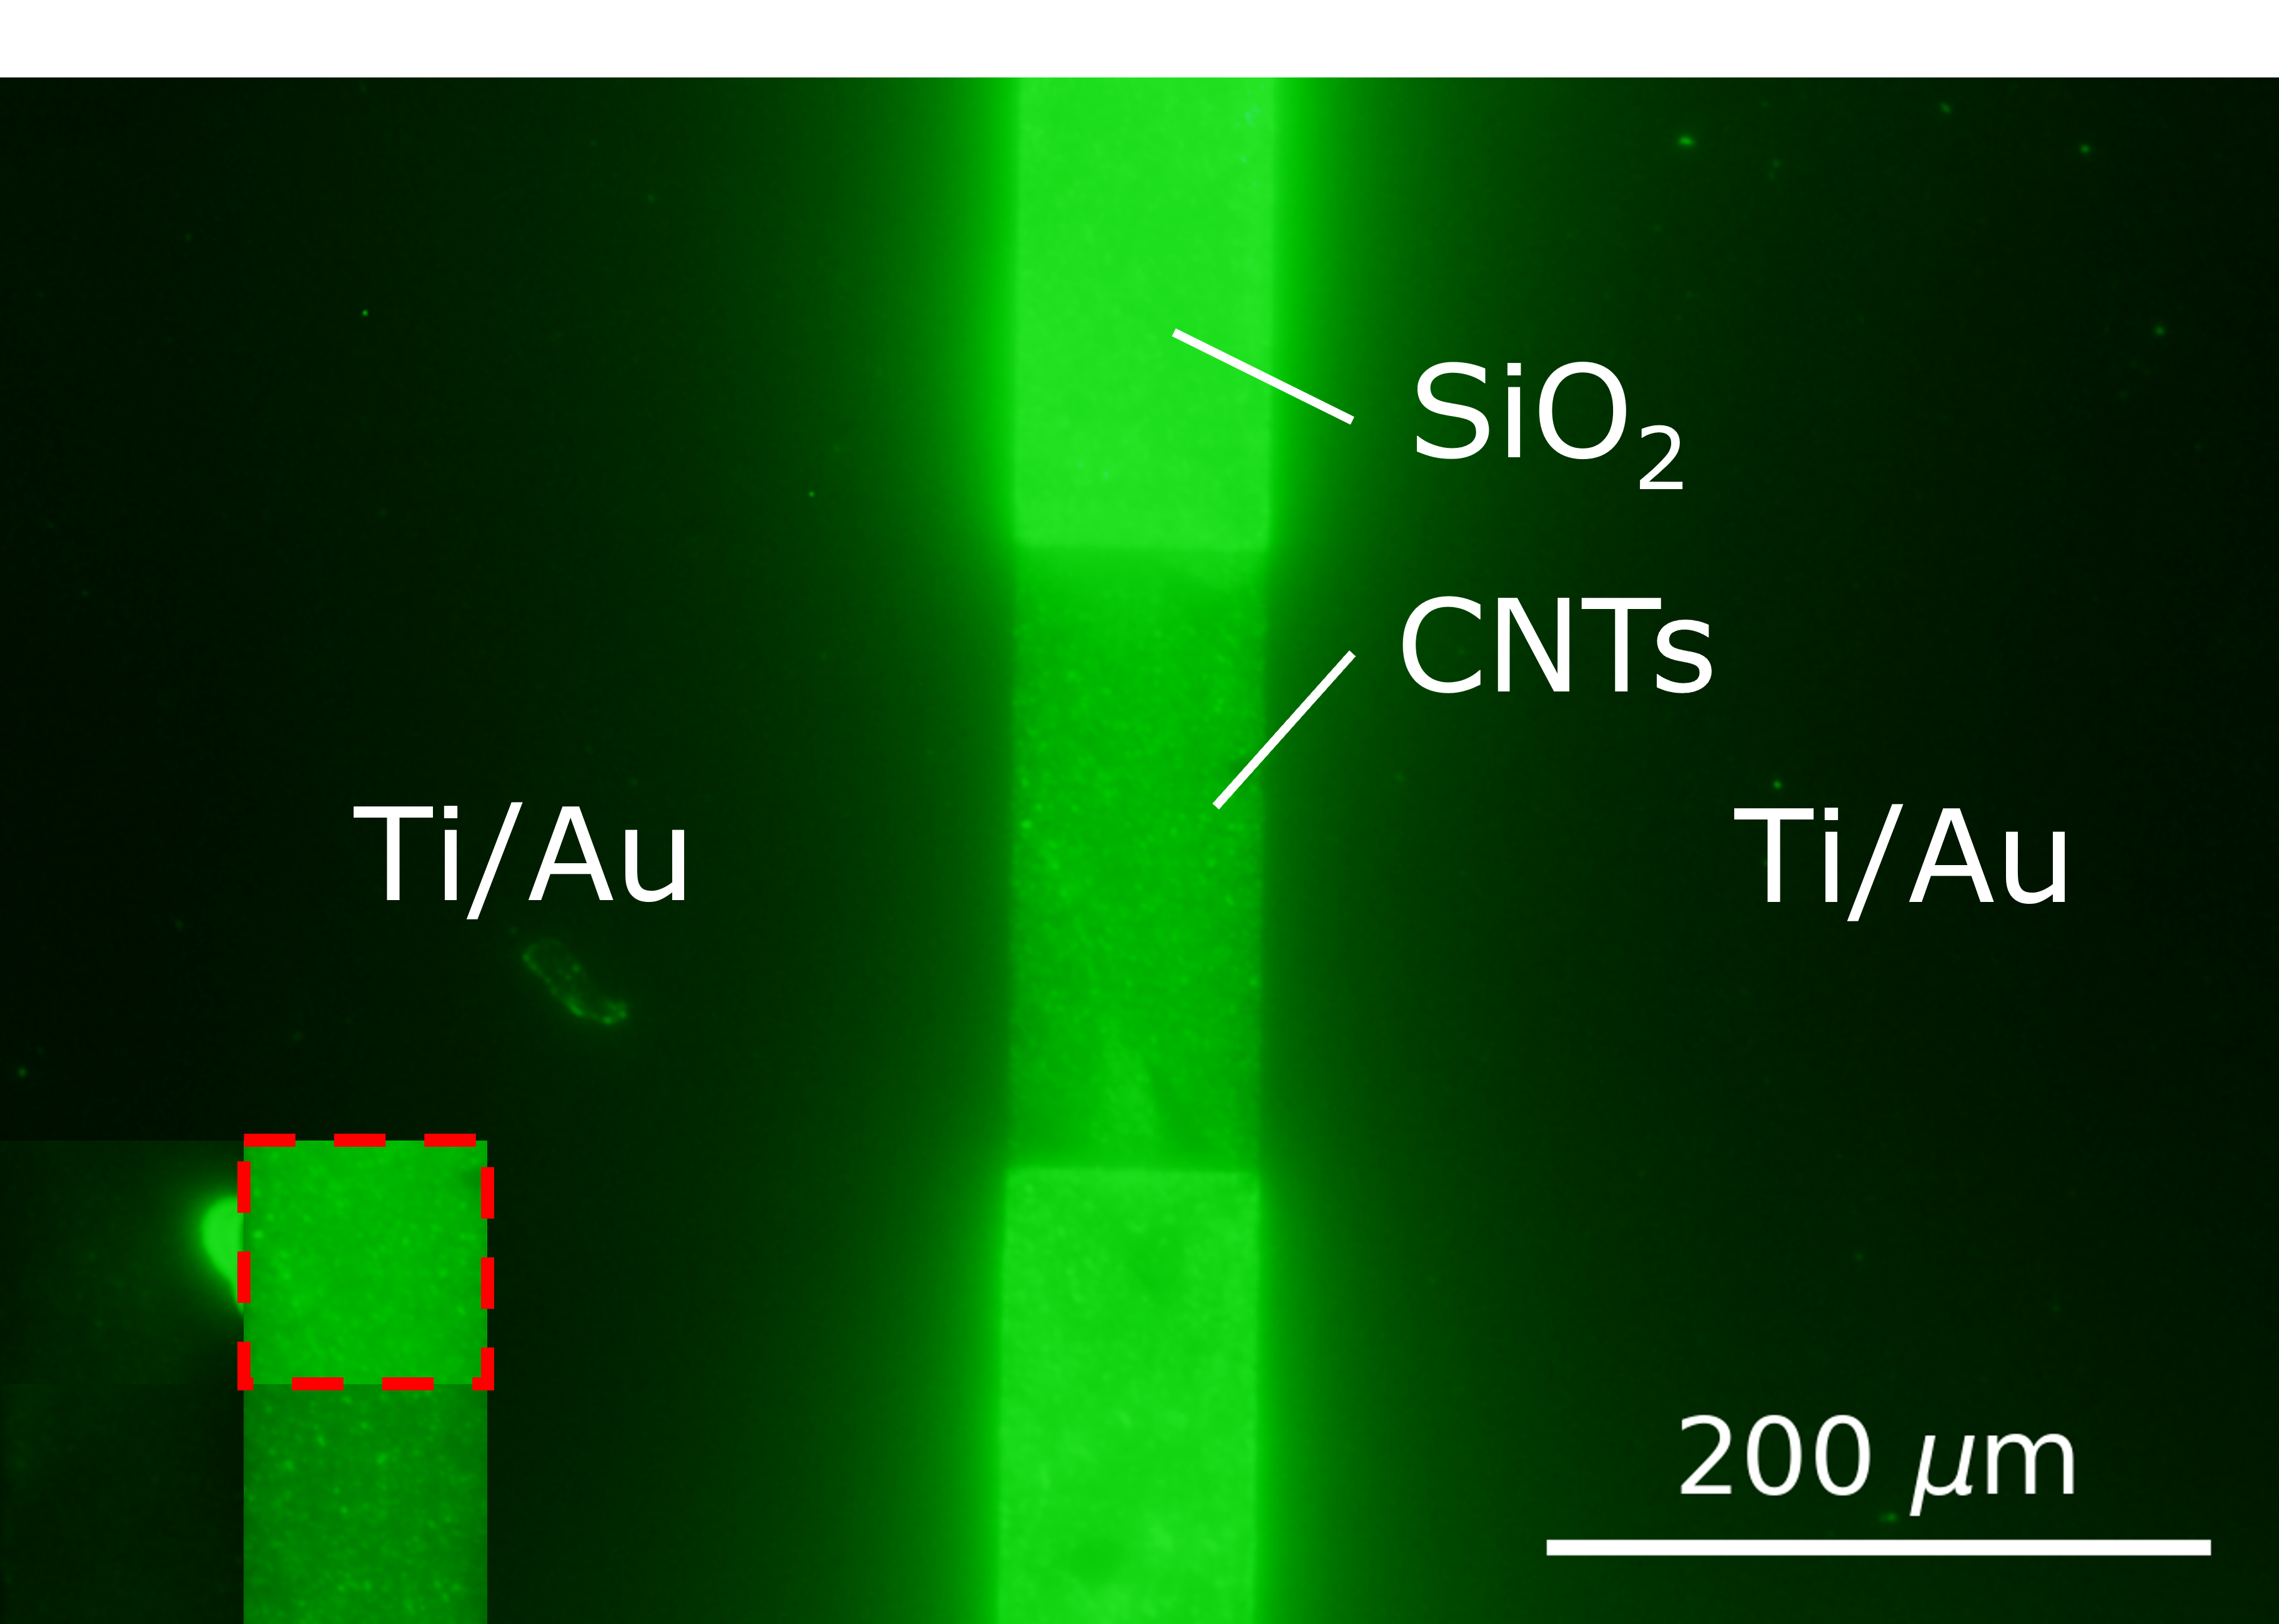
\includegraphics{figures/ch7/modified_GFPOR_PBASE_10sexposure_40X_mediumcontrast_ch1_231019_2.png}

}

}

\end{minipage}%
%
\begin{minipage}[t]{0.01\linewidth}

{\centering 

~

}

\end{minipage}%
\newline
\begin{minipage}[t]{0.03\linewidth}

{\centering 

\raisebox{-\height}{


\includegraphics{figures/(e).png}

}

}

\end{minipage}%
%
\begin{minipage}[t]{0.01\linewidth}

{\centering 

~

}

\end{minipage}%
%
\begin{minipage}[t]{0.45\linewidth}

{\centering 

\raisebox{-\height}{

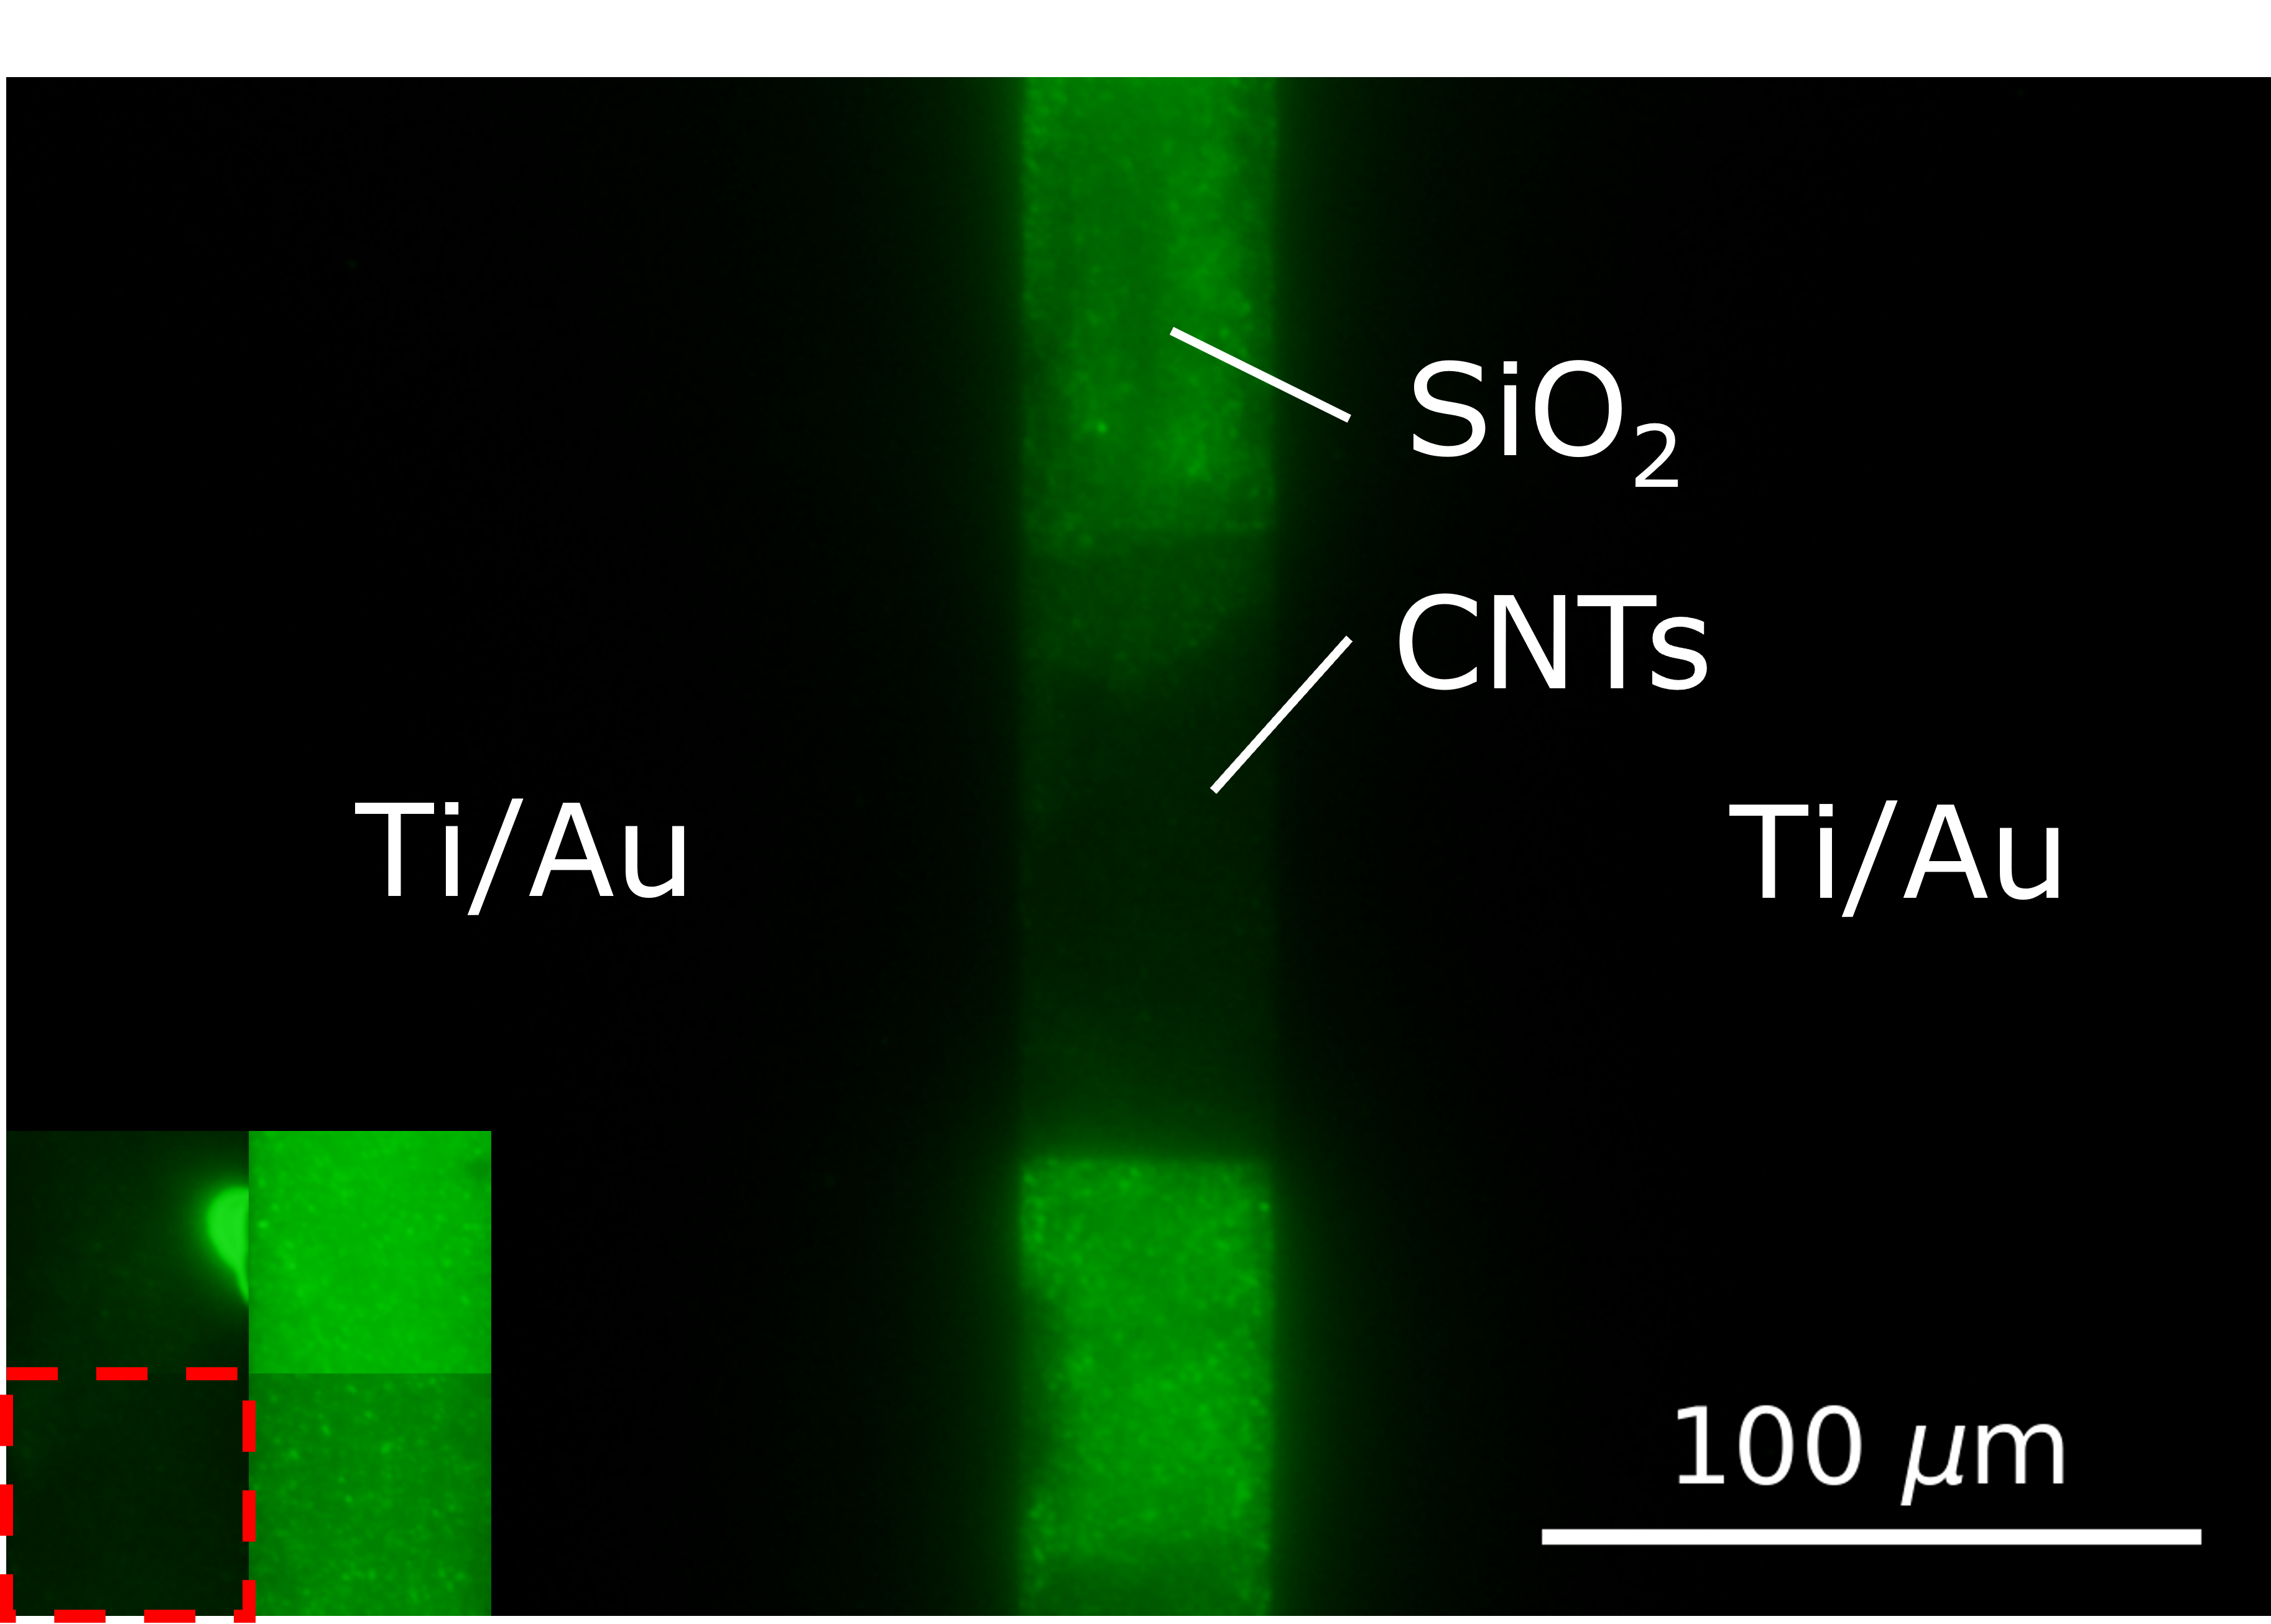
\includegraphics{figures/ch7/modified_GFPOR_10sexposure_40X_mediumcontrast_ch3_240208.png}

}

}

\end{minipage}%
%
\begin{minipage}[t]{0.01\linewidth}

{\centering 

~

}

\end{minipage}%
%
\begin{minipage}[t]{0.03\linewidth}

{\centering 

\raisebox{-\height}{


\includegraphics{figures/(f).png}

}

}

\end{minipage}%
%
\begin{minipage}[t]{0.01\linewidth}

{\centering 

~

}

\end{minipage}%
%
\begin{minipage}[t]{0.45\linewidth}

{\centering 

\raisebox{-\height}{

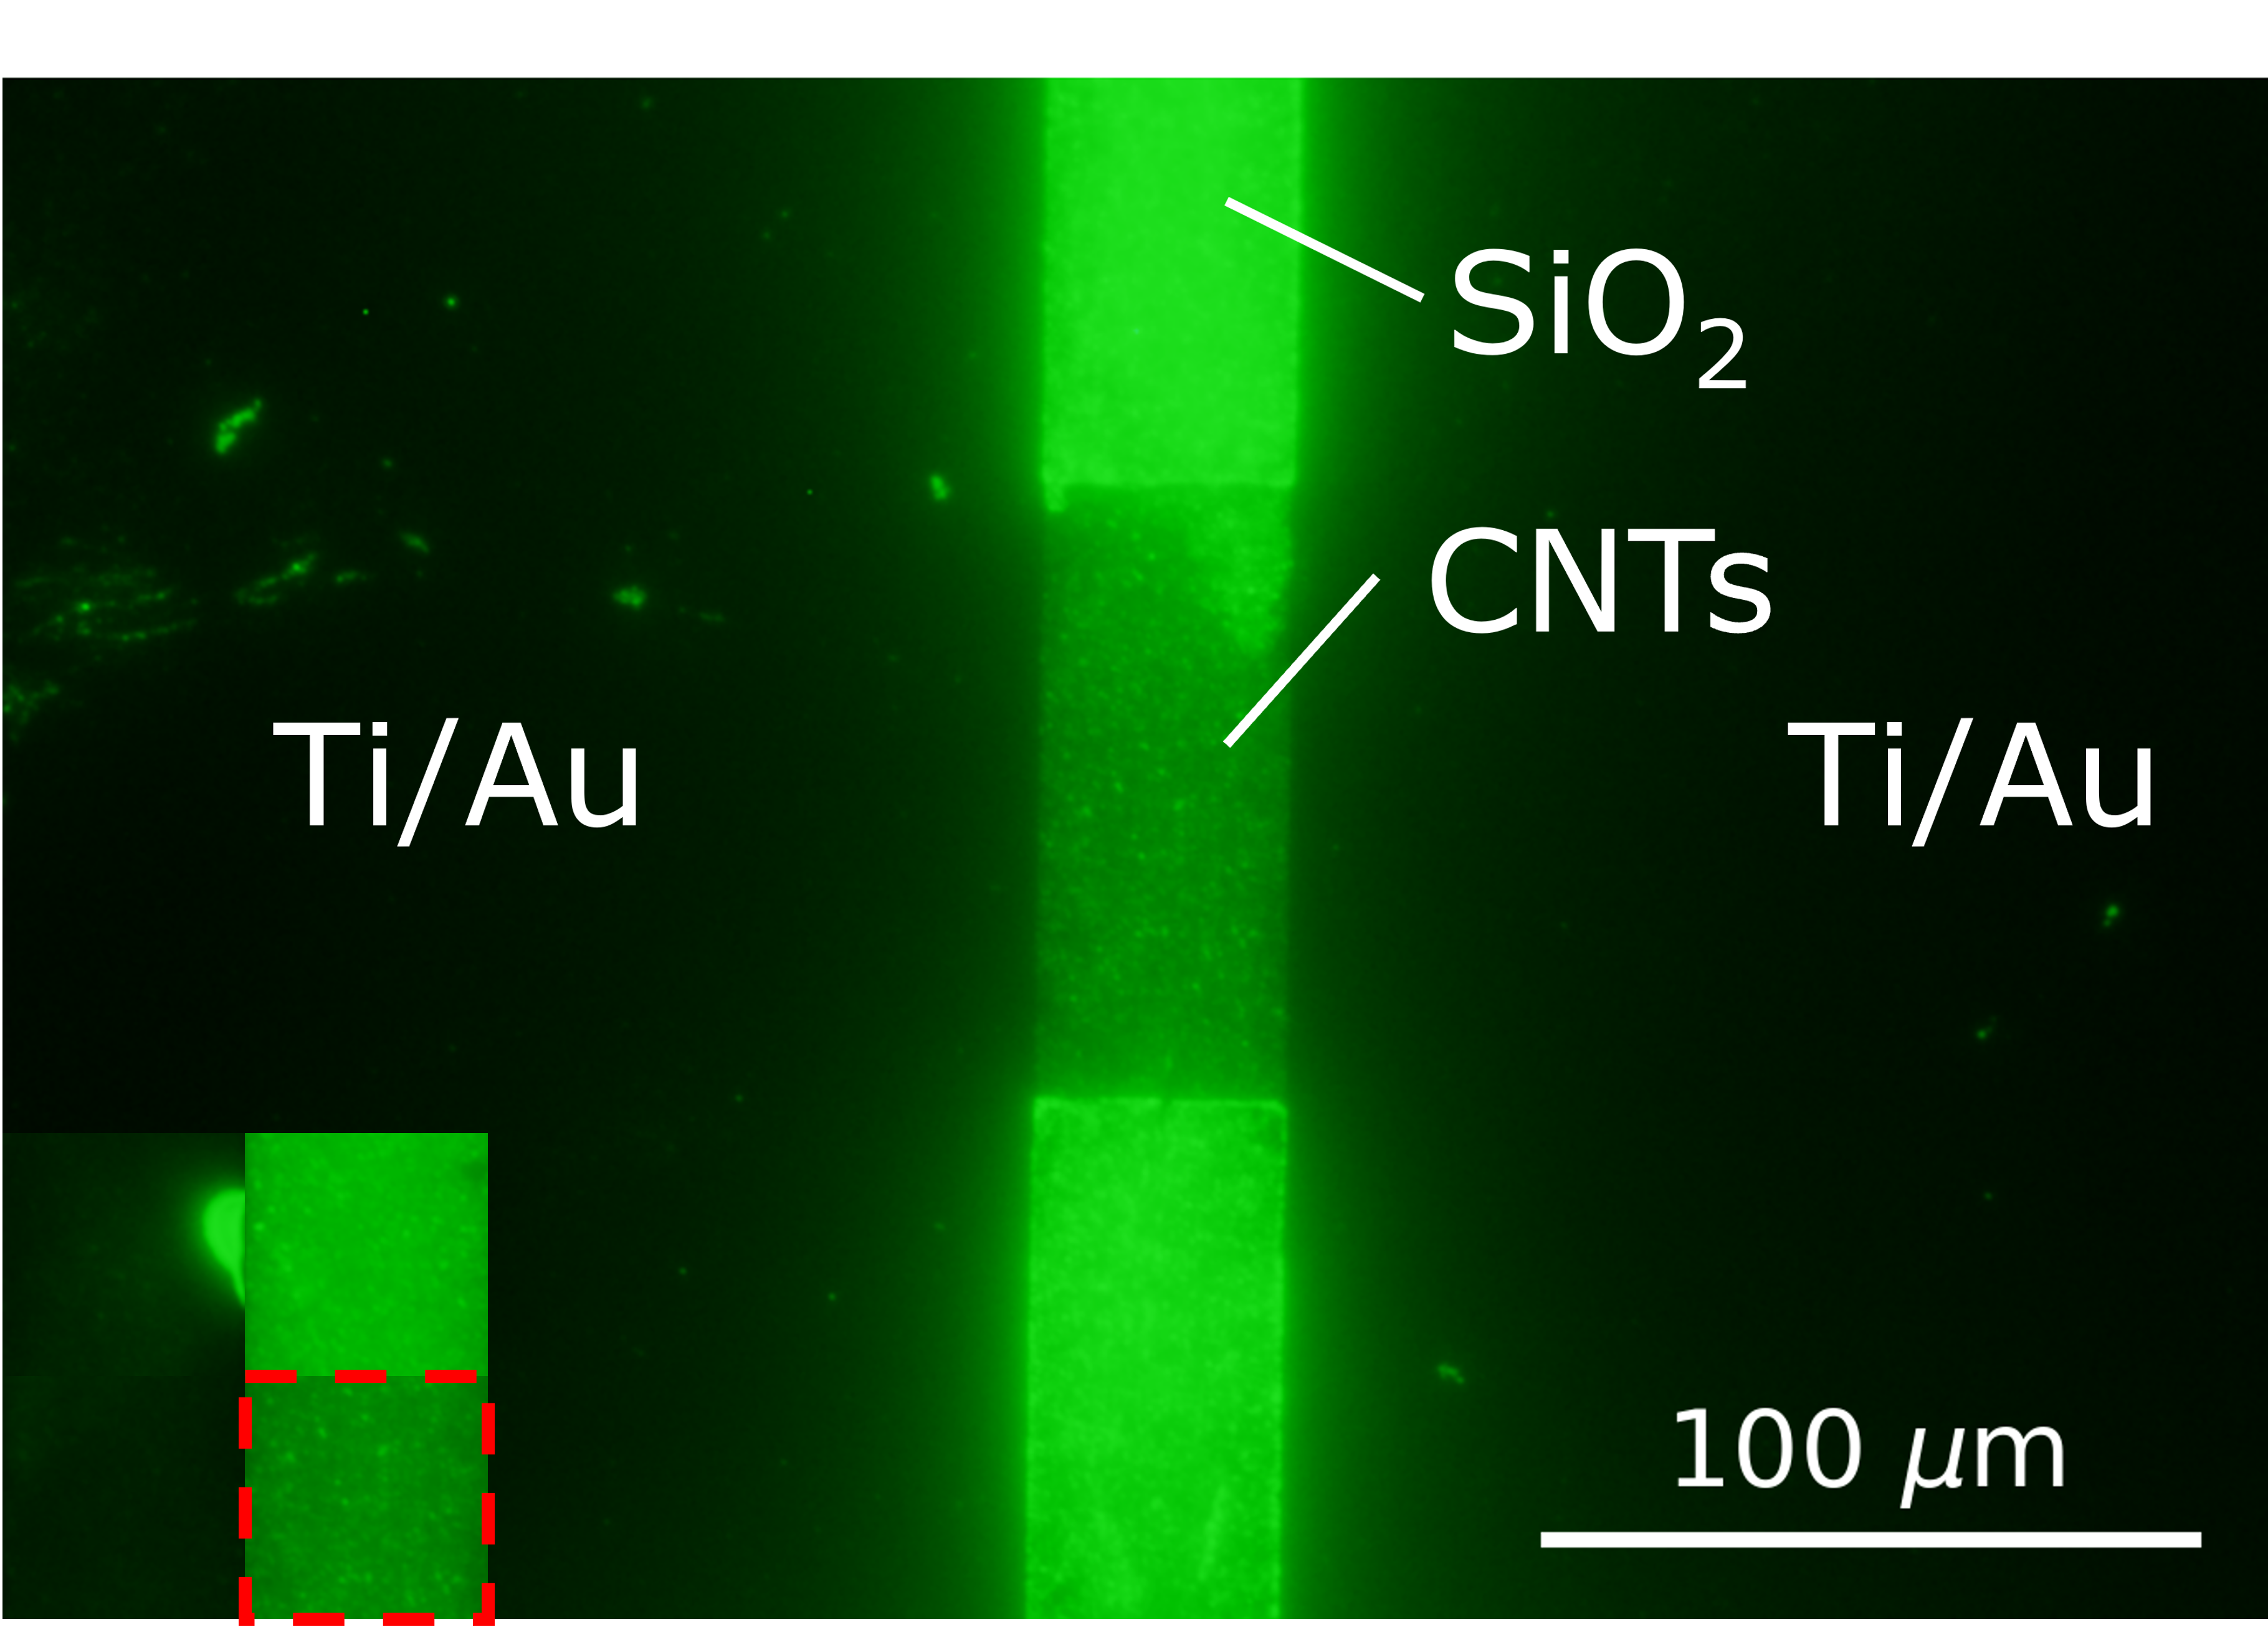
\includegraphics{figures/ch7/modified_GFPOR_PBASE_10sexposure_40X_mediumcontrast_ch2_231019.png}

}

}

\end{minipage}%
%
\begin{minipage}[t]{0.01\linewidth}

{\centering 

~

}

\end{minipage}%

\caption{\label{fig-PBASE-GFP-ORs}The fluorescence images on the left
side \(-\) (a), (c) and (e) \(-\) show unencapsulated carbon nanotube
network channels from a device incubated in GFP-OR nanodiscs. The
rectangular dark regions to the left and right of each image are the Au
electrodes. The fluorescence images on the right \(-\) (b), (d) and (f)
\(-\) show the channels of a similar device after successive PBASE and
GFP-OR nanodisc incubation. Images (a) and (c) are both of the same
channel on the first device, and images (b) and (d) are of the same
channel on the second, but (c) and (d) were taken using a greater
magnification. The insets in (c)-(f) compare the central channel region
of (c)-(f) more directly. All images were taken with the same microscope
settings (GFP filter and 10 s exposure time), taken in quick succession,
directly after functionalisation in a dark room.}

\end{figure}

Fluorescence microscopy was also used to confirm the presence of odorant
receptors tagged with \emph{Aequorea Victoria} green fluorescent protein
(GFP-ORs) on the carbon nanotube film. A device was functionalised with
GFP-OR nanodiscs using the process described at the beginning of this
section (batch number ND-GFP-OR43b-0002, prepared 12 months earlier).
This functionalisation was performed in darkness, with the odorant
receptor nanodisc vial transported under an opaque cover to protect it
from light. After functionalisation, devices were briefly rinsed with DI
water and nitrogen dried to remove salt residue left by the \(1 \times\)
PBS. A control device was also prepared without the use of PBASE,
skipping steps 3 and 4 in the functionalisation process. Fluorescence
microscope images were taken immediately after functionalisation;
devices were transported to the fluorescence microscope room in a
foil-wrapped container, and the fluorescence microscope room was kept
dark while images were taken. Fluorescence images of the devices are
shown in Figure~\ref{fig-PBASE-GFP-ORs}. The SiO\(_2\) regions in each
image appear bright under the GFP filter, indicating attachment between
the GFP-OR nanodiscs and the SiO\(_2\) substrate has occurred. As the
process from \textbf{?@sec-photoresist-contamination} has been followed,
it is unlikely that the GFP-OR nanodiscs are affixed to residual
photoresist.

A comparison of fluorescence in the channel region between images on the
left of Figure~\ref{fig-PBASE-GFP-ORs} (GFP-OR nanodiscs) and the images
on the right (GFP-OR nanodiscs and PBASE) is given by the inset in
Figure~\ref{fig-PBASE-GFP-ORs} (c)-(f). The inset demonstrates that the
channels not incubated in PBASE are significantly less bright than those
that had been incubated with PBASE. It appears that the presence of
GFP-OR nanodiscs in \(1 \times\) PBS is limited on these channels.
However, when the carbon nanotubes are modified with PBASE, there is
clear attachment of GFP-OR nanodiscs to the channel, and the channel
shows up brightly under the fluorescence microscope. Importantly, since
the GFP is attached to odorant receptors rather than the nanodiscs
themselves, there must be odorant receptors present on the channel after
functionalisation; attachment to the channel is not limited to empty
nanodiscs. This trend was consistent across all conducting channels on
each of the two devices. A similar comparison technique has been used
previously to detect human odorant receptor attachment to a carbon
nanotube network via 1,5-diaminonaphthalene \autocite{Lee2012b}. As far
as I know, this is the first time fluorescence has been used to
investigate the attachment of insect odorant receptor nanodiscs to a
carbon nanotube network.

\hypertarget{sec-EtHex-aqueous-sensing}{%
\subsection{Aqueous Sensing of Ethyl
Hexanoate}\label{sec-EtHex-aqueous-sensing}}

The procedure used for biosensor detection of ethyl hexanoate in liquid
was the same as the procedure outlined in \textbf{?@sec-dummy-sensing},
except 0.5\% v/v DMSO was present in the buffer solution (to improve
ethyl hexanoate solubility \autocite{Galvao2014}) and dilutions of ethyl
hexanoate in the same 0.5\% v/v DMSO \(1 \times\) PBS were added during
the sensing series. Dilutions of 1 fM, 1 pM, 1 nM and 1 µM ethyl
hexanoate in 0.5\% v/v DMSO \(1 \times\) PBS were prepared before device
characterisation according to Table~\ref{tbl-dilution-preparation},
using pre-prepared concentrations of 200 fM, 200 pM, 200 nM and 200 µM
ethyl hexanoate in DMSO. The ethyl hexanoate in DMSO dilutions were
prepared beforehand as a 1:10 dilution series in DMSO using 200 mM stock
solution, where dilutions ranged from 20 mM to 200 fM. Sampling
measurements were taken using the B1500A semiconductor device analyser,
with the transfer measurement in Figure~\ref{fig-OR22a-TX-comparison}
(b) taken directly before sensing. The full control series plus sensing
sequence is shown in Figure~\ref{fig-EtHex-aqueous-sensing}. Gate
current remained negligible across the entire sensing procedure.

\hypertarget{tbl-dilution-preparation}{}
\begin{longtable}[t]{>{\raggedright\arraybackslash}p{3.2cm}>{\raggedright\arraybackslash}p{2.5cm}>{\raggedright\arraybackslash}p{2.5cm}>{\raggedright\arraybackslash}p{4.2cm}}
\caption{\label{tbl-dilution-preparation}Preparation of analyte dilutions in 1X PBS from solutions of analyte in
DMSO. The 1X PBS used was prepared on the same day as the dilution
process. }\tabularnewline

\toprule
Conc. in DMSO & 1XPBS added & Final volume & Final conc.\\
\midrule
5 µL × 0 fM & 995 µL & 1 mL & 0 fM, 0.5\% v/v DMSO\\
5 µL × 200 fM & 995 µL & 1 mL & 1 fM, 0.5\% v/v DMSO\\
5 µL × 200 pM & 995 µL & 1 mL & 1 pM, 0.5\% v/v DMSO\\
5 µL × 200 nM & 995 µL & 1 mL & 1 nM, 0.5\% v/v DMSO\\
5 µL × 200 µM & 995 µL & 1 mL & 1 µM, 0.5\% v/v DMSO\\
\bottomrule
\end{longtable}

\begin{figure}

{\centering 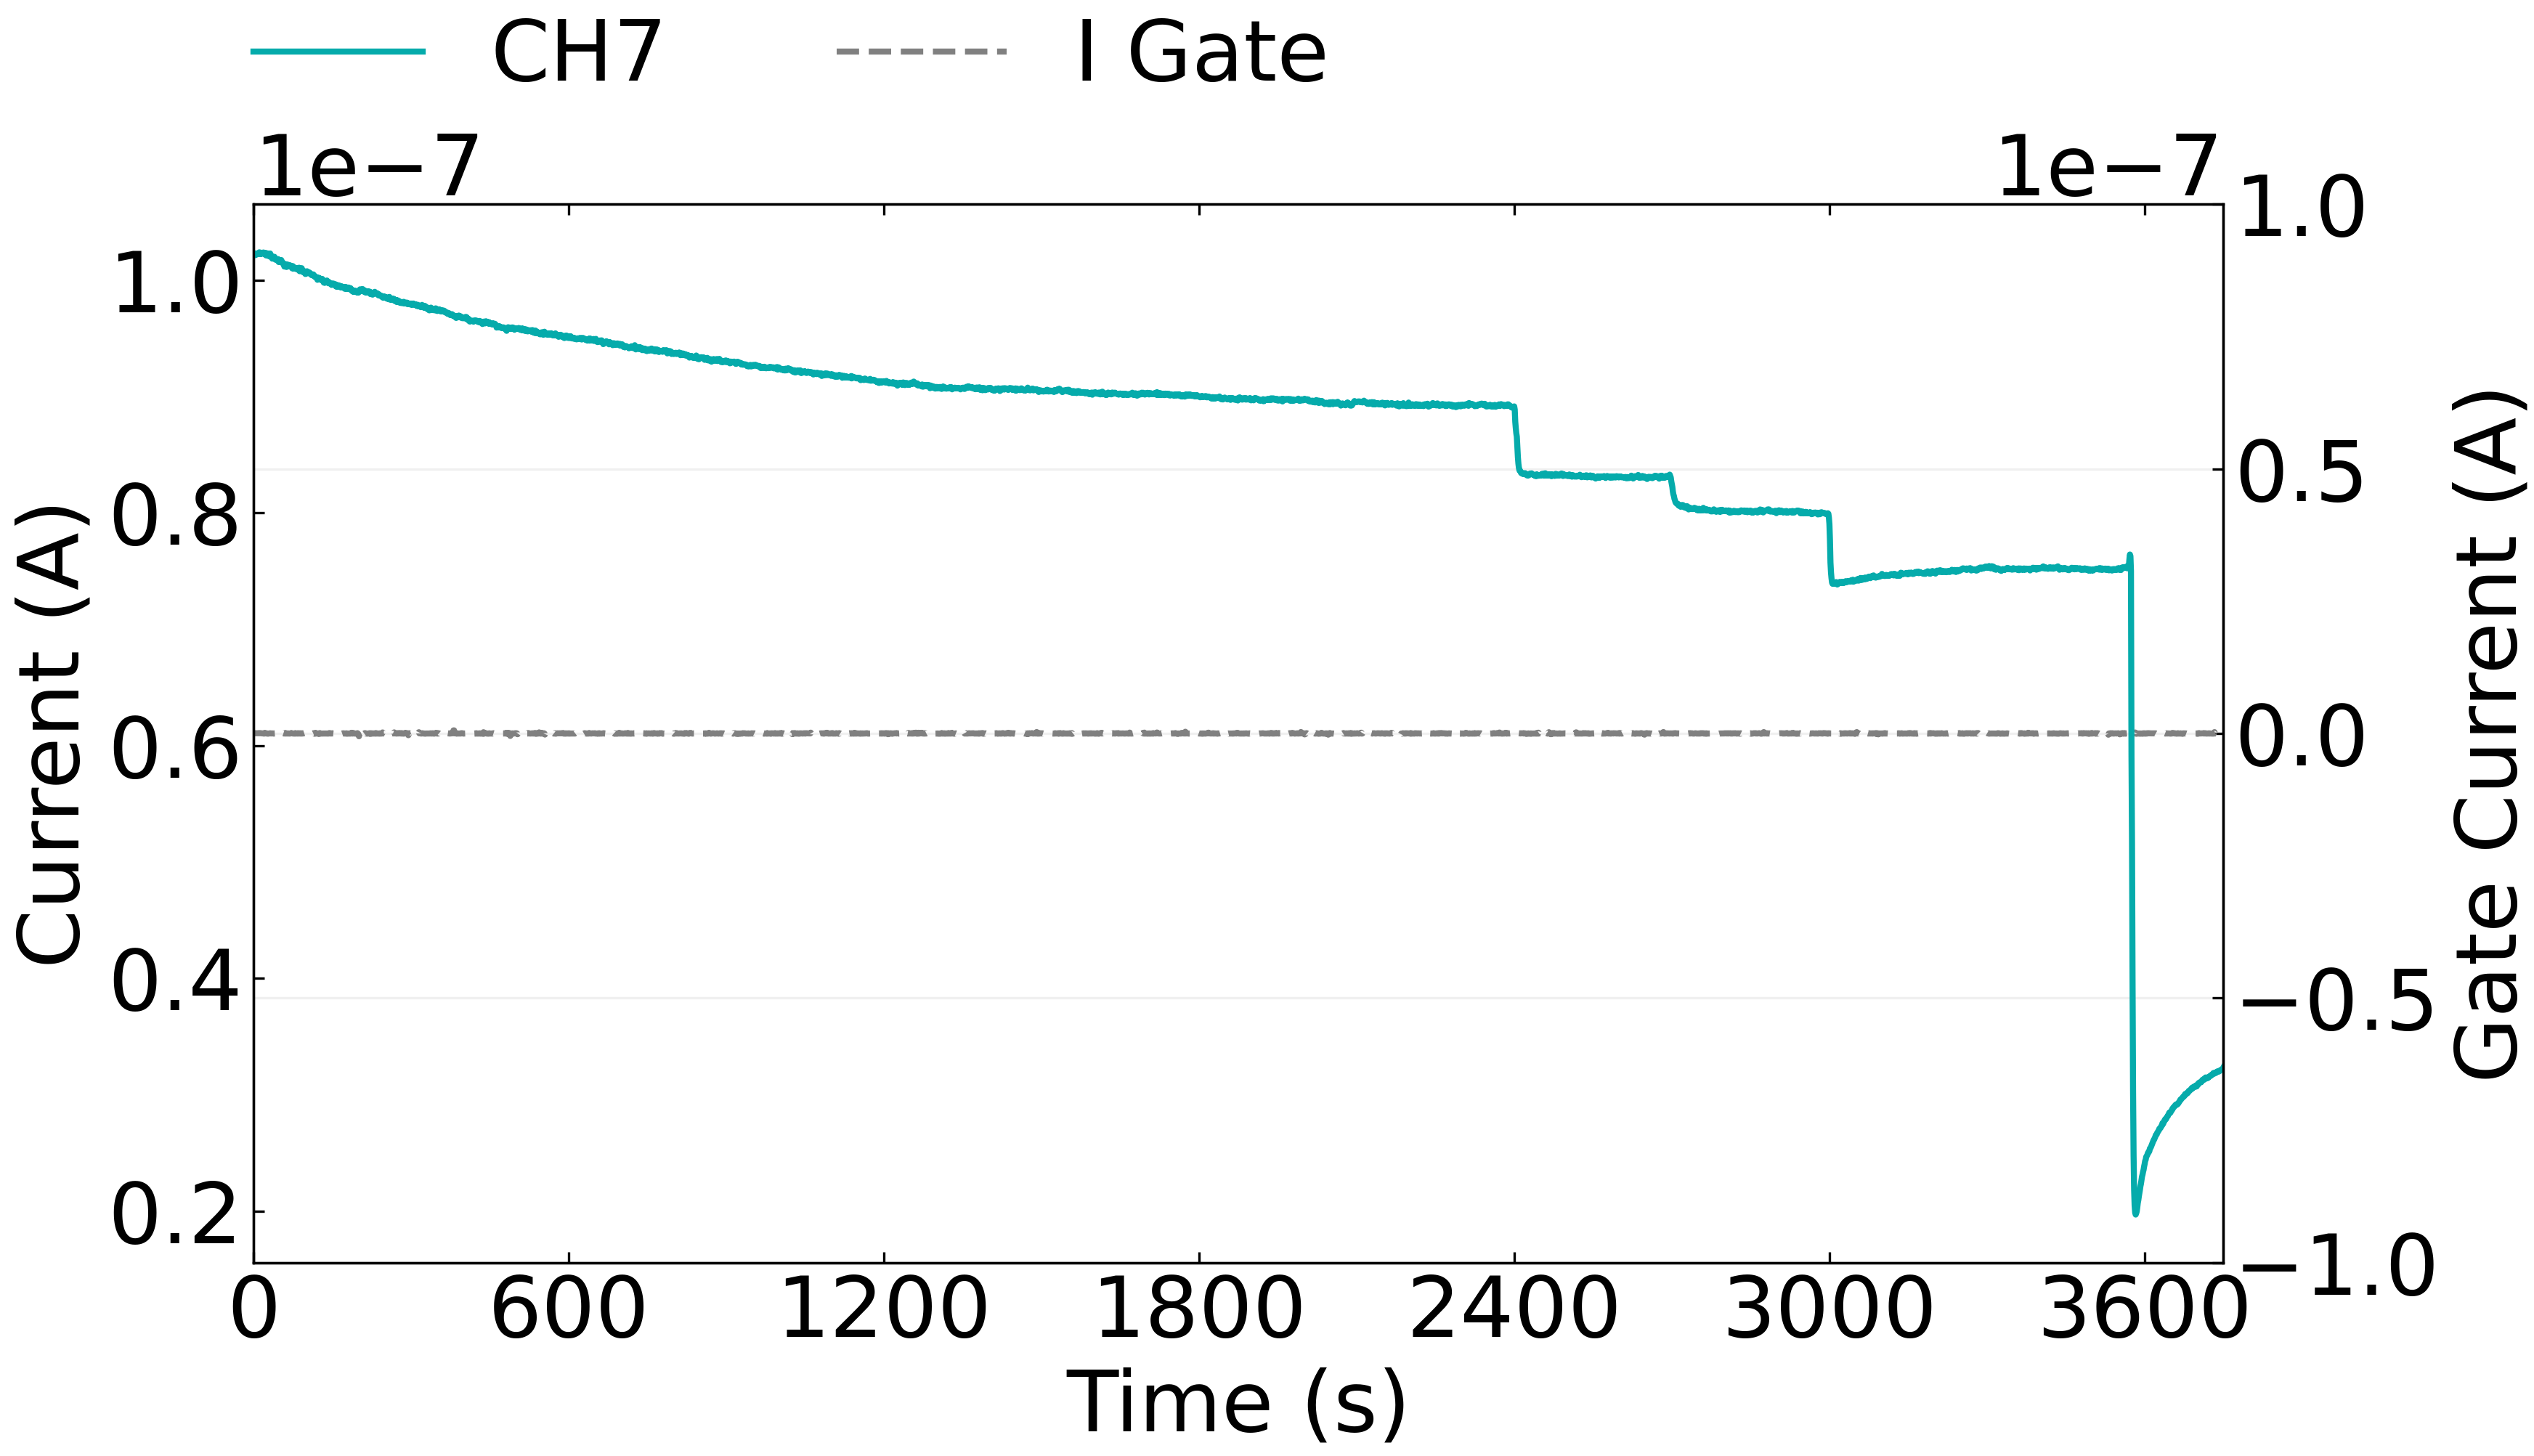
\includegraphics[width=0.7\textwidth,height=\textheight]{figures/ch7/Q1C6.png}

}

\caption{\label{fig-EtHex-aqueous-sensing}The control series (\(0-1800\)
s) and ethyl hexanoate sensing series (\(1800-3900\)) of the
OR22a-functionalised device channel. Source-drain voltage was set at
\(V_{ds}\) = 100 mV while gate voltage was set at \(V_g\) = 0 V.
Functionalisation and sensing was performed using the methods developed
in this thesis by Danica Fontein, School of Chemical and Physical
Sciences, Te Herenga Waka - Victoria University of Wellington.}

\end{figure}

\begin{figure}

\begin{minipage}[t]{0.11\linewidth}

{\centering 

~

}

\end{minipage}%
%
\begin{minipage}[t]{0.03\linewidth}

{\centering 

\raisebox{-\height}{


\includegraphics{figures/(a).png}

}

}

\end{minipage}%
%
\begin{minipage}[t]{0.01\linewidth}

{\centering 

~

}

\end{minipage}%
%
\begin{minipage}[t]{0.70\linewidth}

{\centering 

\raisebox{-\height}{

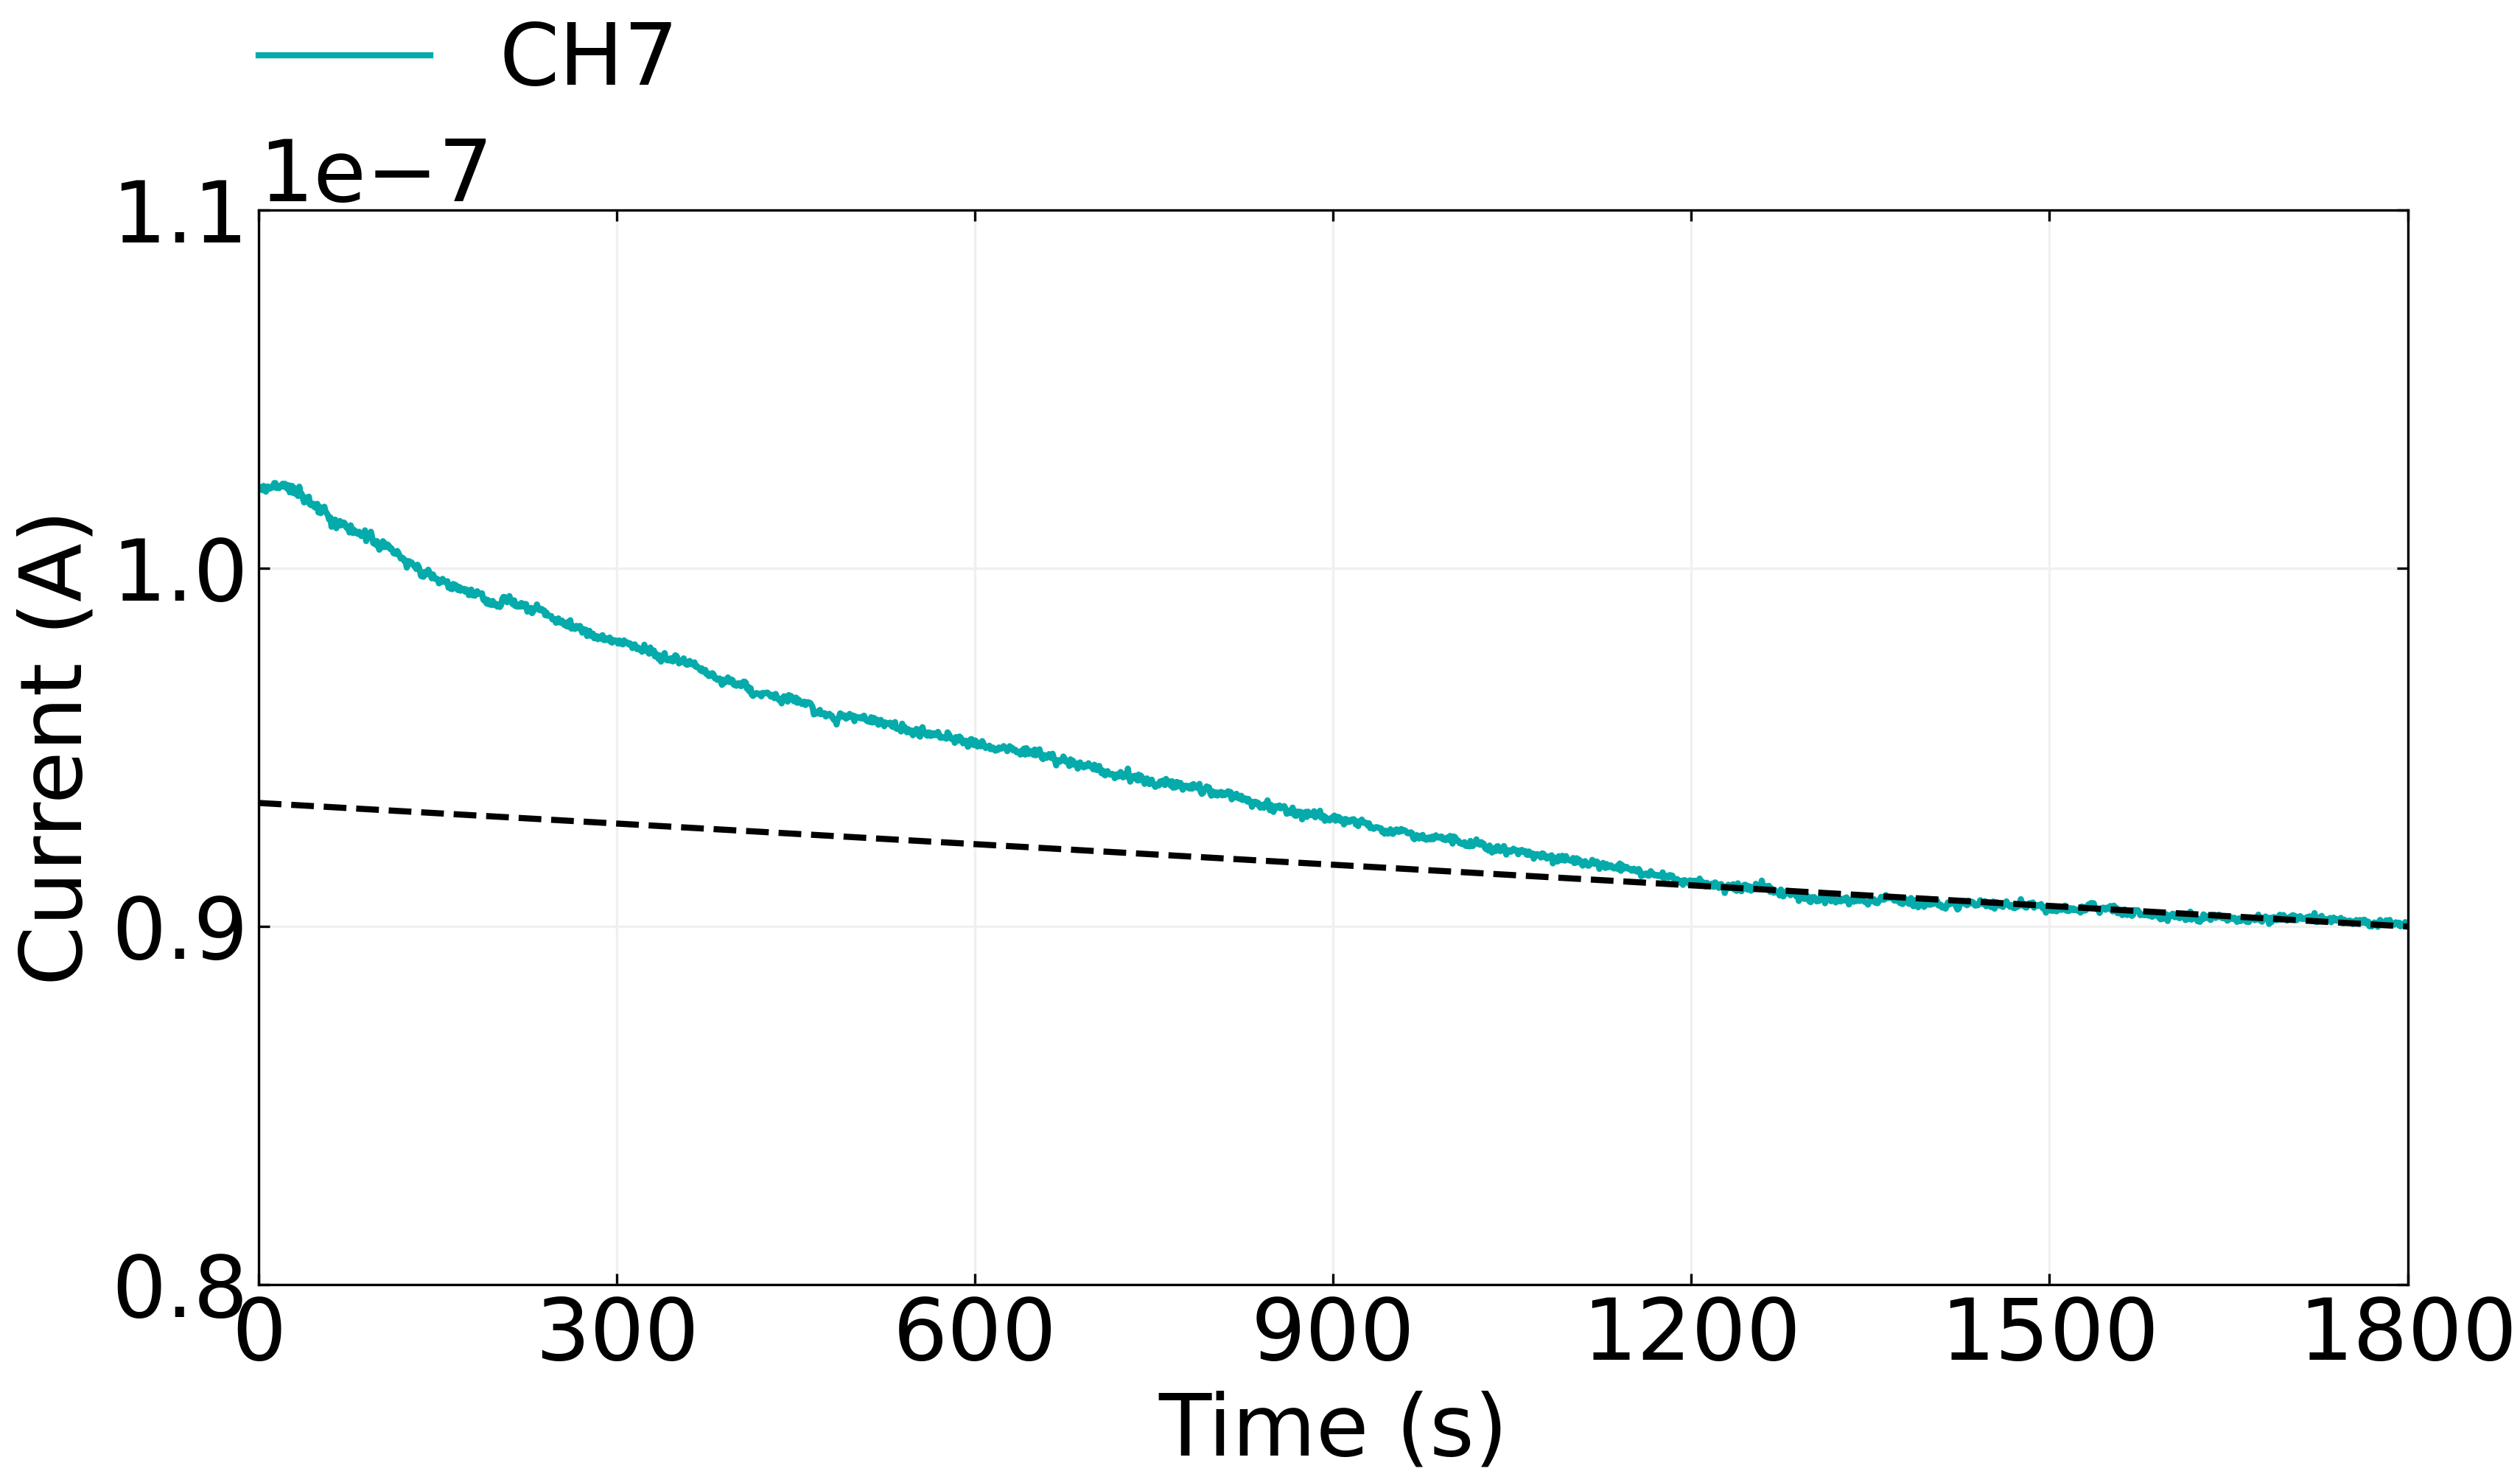
\includegraphics{figures/ch7/Q1C6_with_fitted_curves.png}

}

}

\end{minipage}%
%
\begin{minipage}[t]{0.15\linewidth}

{\centering 

~

}

\end{minipage}%
\newline
\begin{minipage}[t]{0.11\linewidth}

{\centering 

~

}

\end{minipage}%
%
\begin{minipage}[t]{0.03\linewidth}

{\centering 

\raisebox{-\height}{


\includegraphics{figures/(b).png}

}

}

\end{minipage}%
%
\begin{minipage}[t]{0.01\linewidth}

{\centering 

~

}

\end{minipage}%
%
\begin{minipage}[t]{0.70\linewidth}

{\centering 

\raisebox{-\height}{

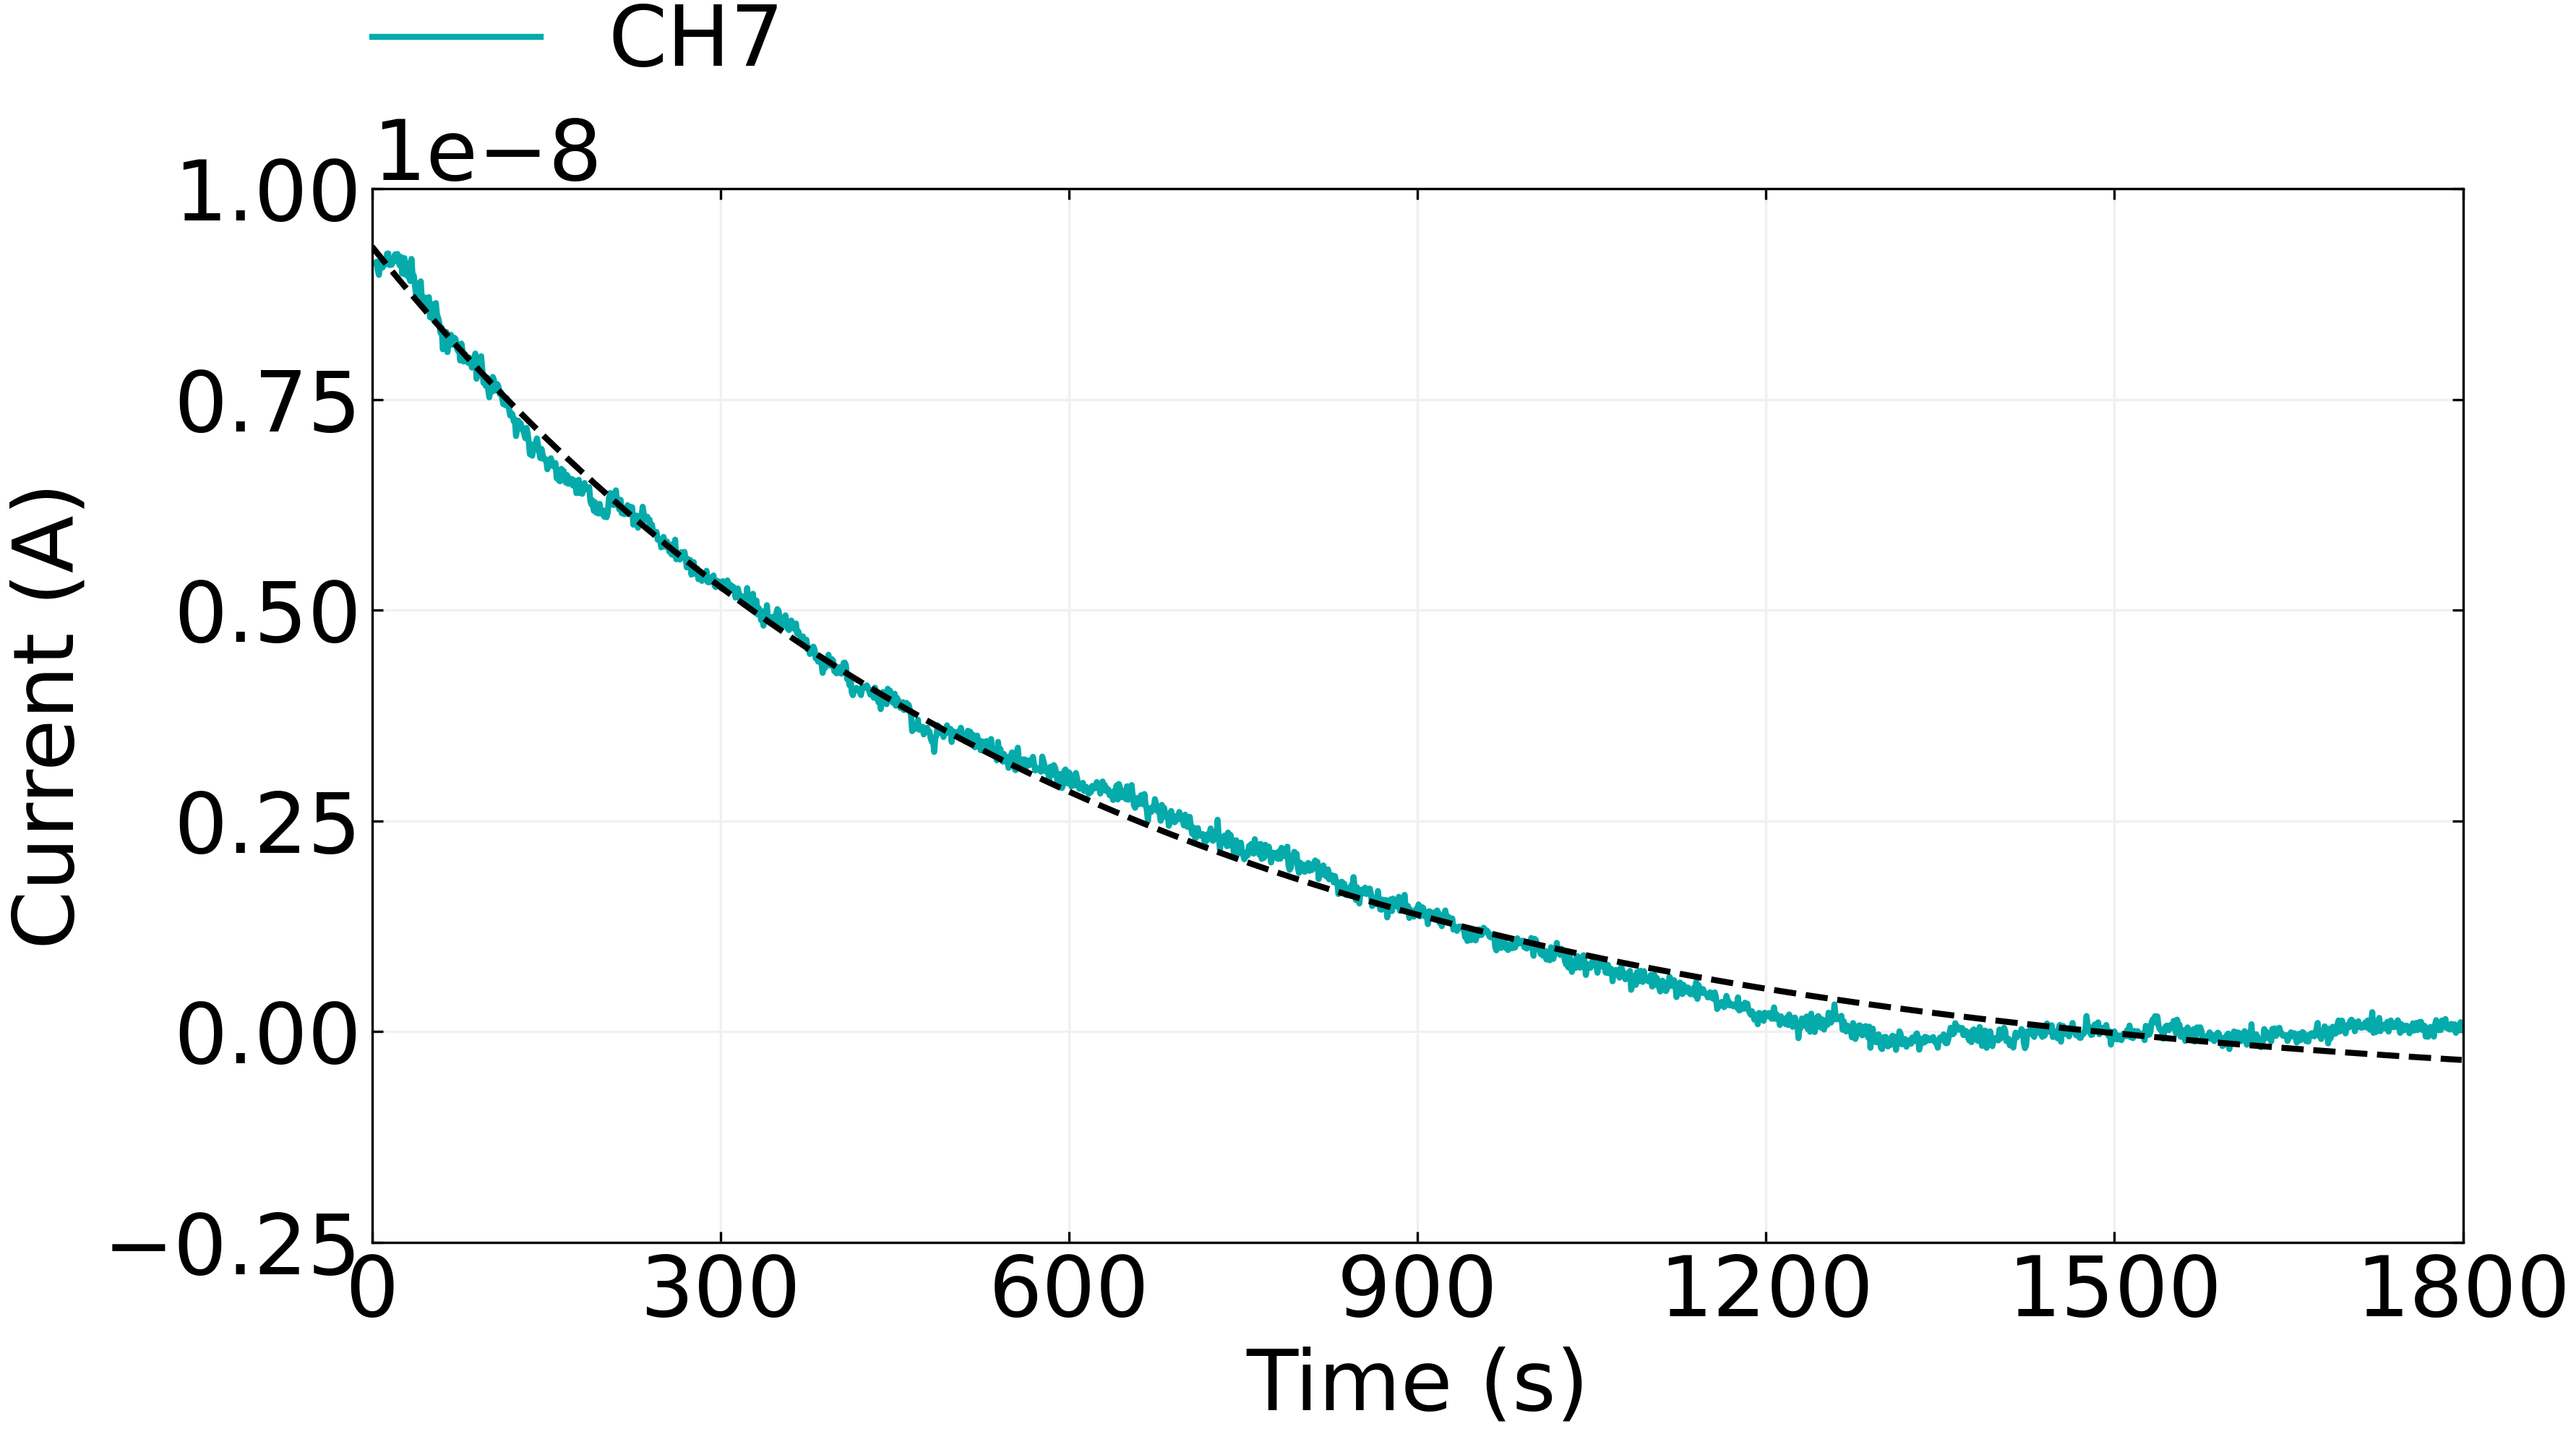
\includegraphics{figures/ch7/Q1C6_with_fitted_curves_exp.png}

}

}

\end{minipage}%
%
\begin{minipage}[t]{0.15\linewidth}

{\centering 

~

}

\end{minipage}%
\newline
\begin{minipage}[t]{0.11\linewidth}

{\centering 

~

}

\end{minipage}%
%
\begin{minipage}[t]{0.03\linewidth}

{\centering 

\raisebox{-\height}{


\includegraphics{figures/(c).png}

}

}

\end{minipage}%
%
\begin{minipage}[t]{0.01\linewidth}

{\centering 

~

}

\end{minipage}%
%
\begin{minipage}[t]{0.70\linewidth}

{\centering 

\raisebox{-\height}{

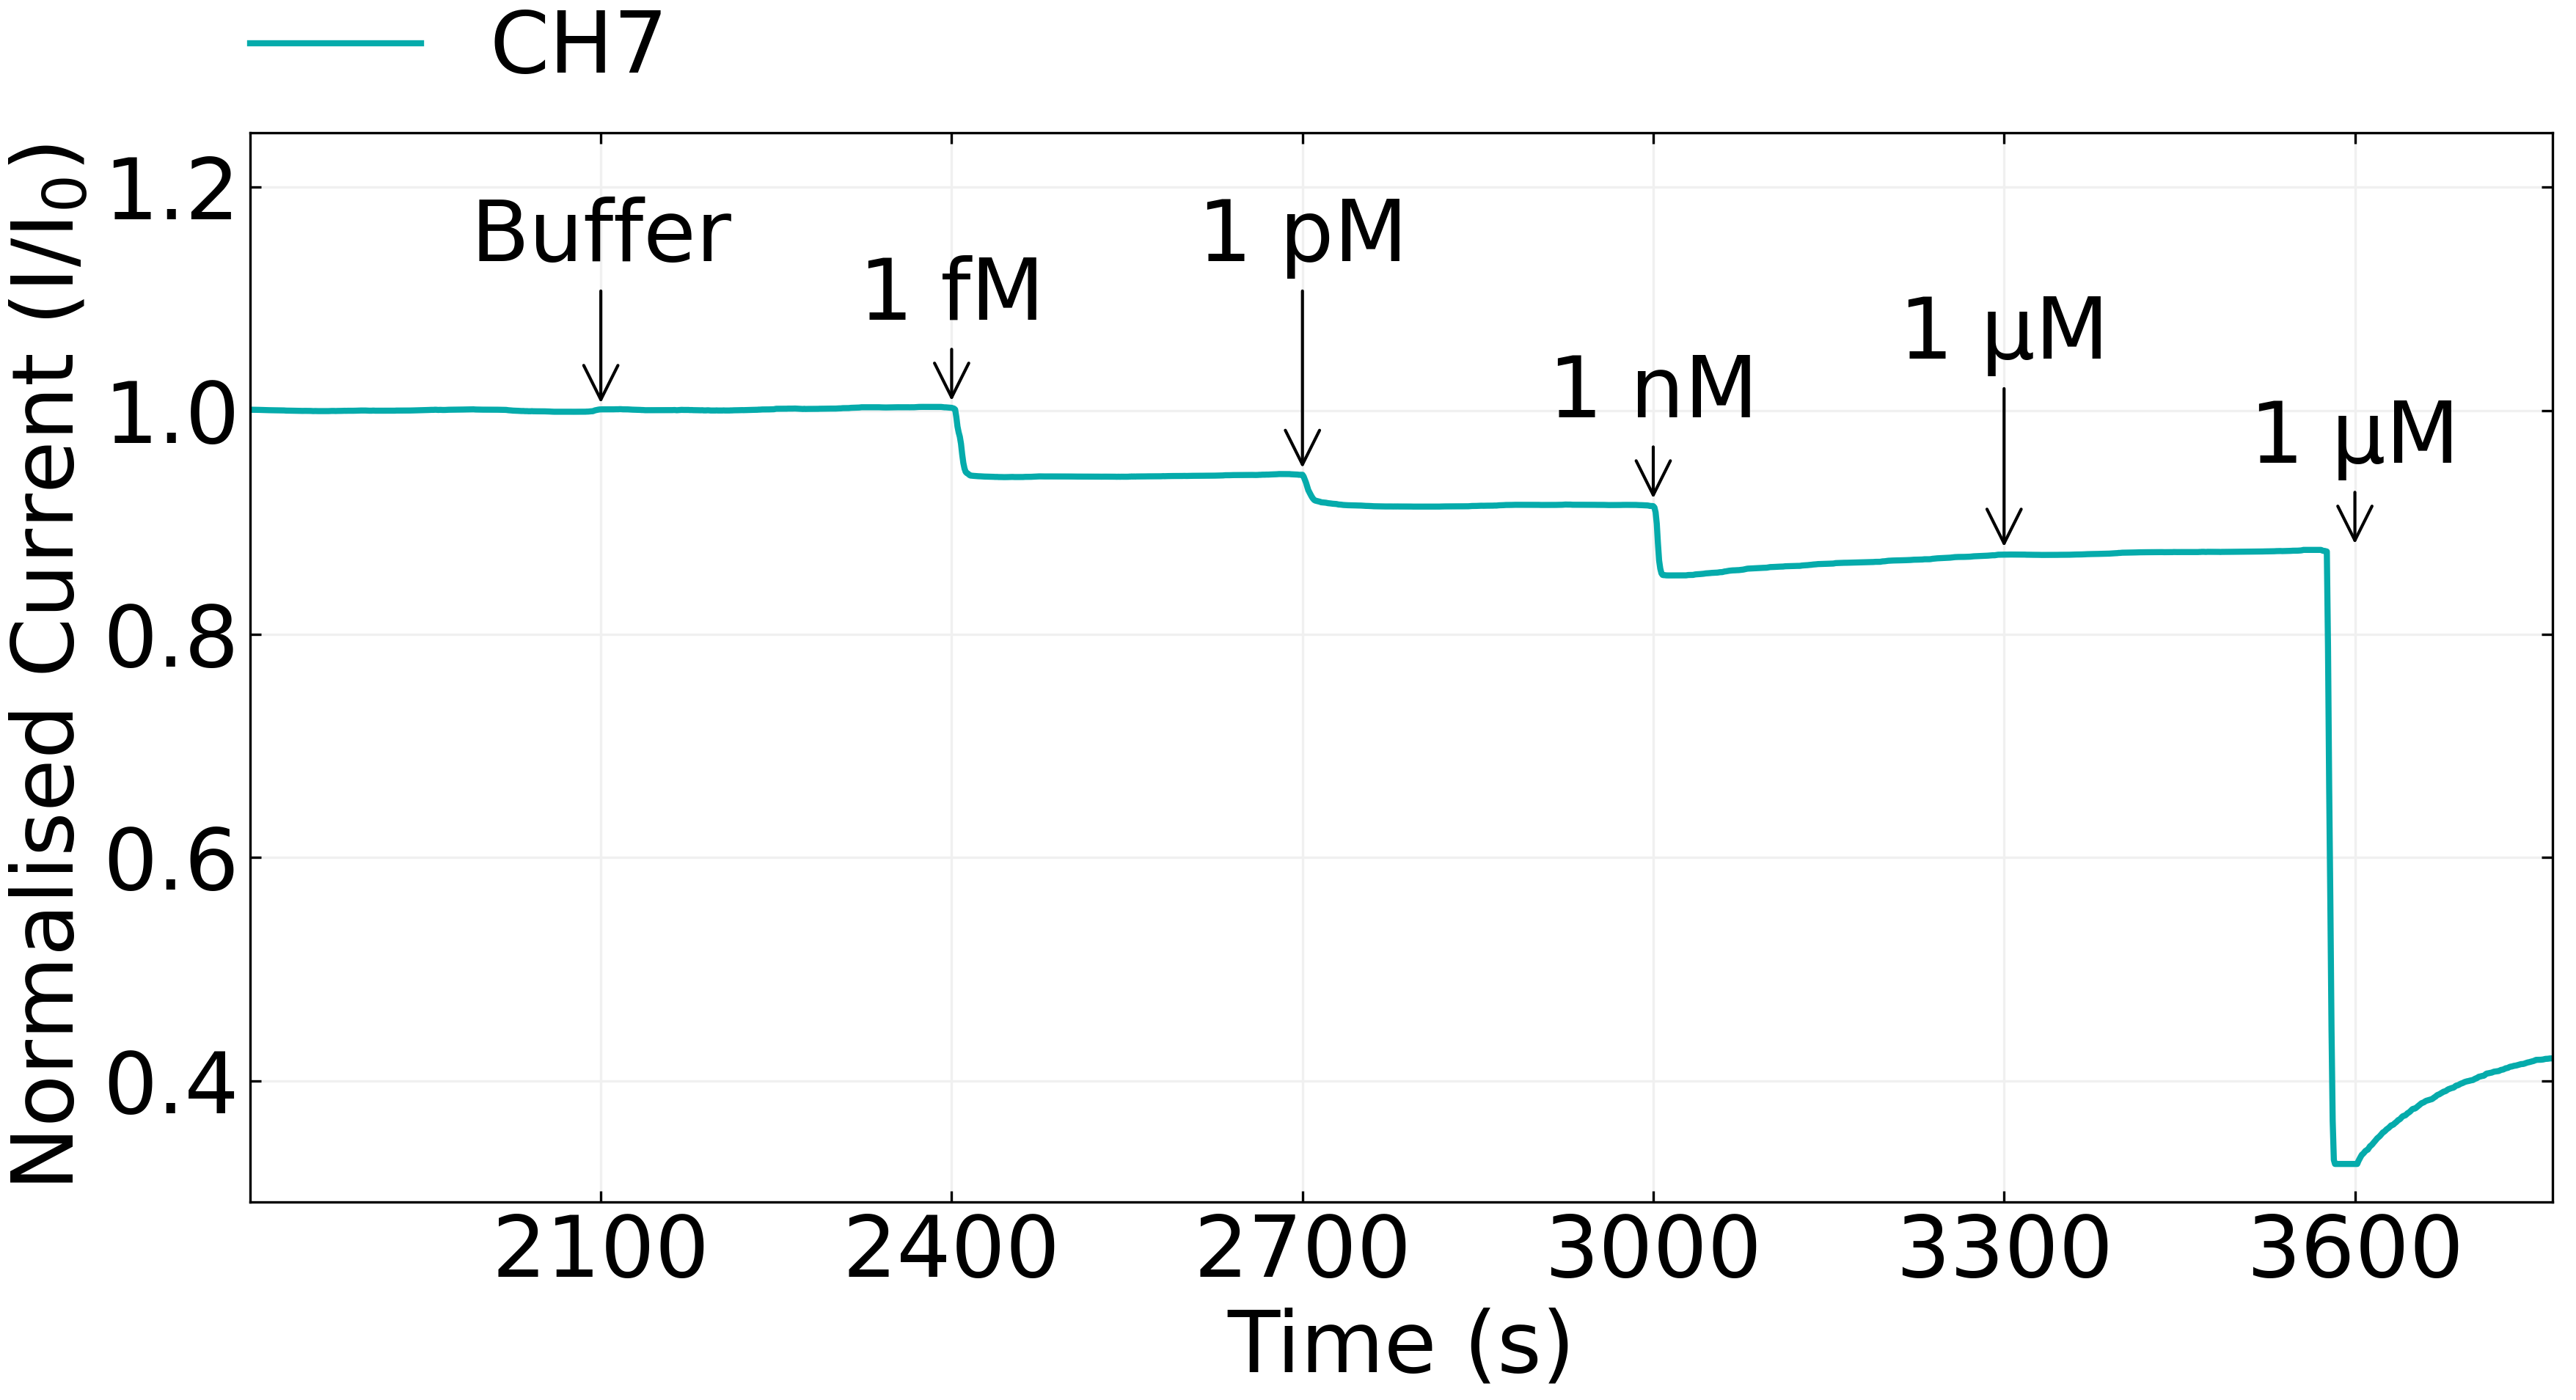
\includegraphics{figures/ch7/Q1C6_filtered_detrend_trunc_arrows_normalised.png}

}

}

\end{minipage}%
%
\begin{minipage}[t]{0.15\linewidth}

{\centering 

~

}

\end{minipage}%

\caption{\label{fig-OR22a-series}The control series of the
OR22a-functionalised device is shown in (a) alongside an extrapolated
linear fit from 1200 s onwards. The control series with the linear
approximation subtracted is shown in (b), where an exponential curve has
been fitted. The normalised ethyl hexanoate sensing series is shown in
(c) with baseline drift substracted and a moving median filter applied.
The concentration of each 20 µL addition is indicated above the time of
addition. Across both the control series and sensing series, \(V_{ds}\)
= 100 mV and \(V_g\) = 0 V.}

\end{figure}

The control series for the sensing series is shown in
Figure~\ref{fig-OR22a-series} (a). No clear stepwise response is seen to
PBS additions or subtractions. The functionalised device shows similar
baseline drift behaviour to that of a pristine device, with a period of
short-term decay quickly yielding to a more long-lived decay behaviour.
A linear fit \(I = c_1t + c_2\) to the region \(1200-1800\) s had a
gradient of \(c_1 = -1.76\pm0.02\) pA/s. This gradient is smaller than
the range of values found for the linear fit approximating the
longer-term drift of a pristine device (\textbf{?@sec-baseline-drift}),
but of the same order of magnitude. The linear fit was then subtracted
from the control series and an exponential fit \(I = I_0\exp(-t/\tau)\)
was performed on the remaining dataset from 0-1200 s, as shown in
Figure~\ref{fig-OR22a-series} (b). A value of \(660 \pm 10\) s was found
for the exponential time constant, similar to those found for the
channels of the pristine device. This confirms that the 1800 s control
series is sufficient to avoid the presence of short-term decay during
sensing.

Figure~\ref{fig-OR22a-series} (c) shows the cleaned and filtered ethyl
hexanoate sensing data from the OR22a-functionalised device from 1800 s
onwards. The concentration of each 20 µL addition is indicated above the
corresponding addition time. The actual concentration in the liquid-gate
well is determined by both the concentration of analyte being added and
the volume of 1X PBS 0.5\% v/v DMSO already present. The concentration
of ethyl hexanoate in the well after each addition is shown in
Table~\ref{tbl-concentrations}. With each addition of ethyl hexanoate, a
subsequent rapid drop in source-drain current across the channel was
observed. This current decrease appears irreversible, as the current
stabilises after each addition at a lower current level than prior to
the addition. As in previous works, all responses were observed without
requiring an ORCO coreceptor present
\autocite{Murugathas2019a,Murugathas2020,Khadka2019,Cheema2021}.

\hypertarget{tbl-concentrations}{}
\begin{longtable}[t]{>{\raggedright\arraybackslash}p{3.2cm}>{\raggedright\arraybackslash}p{1.4cm}>{\raggedright\arraybackslash}p{1.4cm}>{\raggedright\arraybackslash}p{1.4cm}>{\raggedright\arraybackslash}p{1.4cm}>{\raggedright\arraybackslash}p{1.4cm}>{\raggedright\arraybackslash}p{1.4cm}}
\caption{\label{tbl-concentrations}Comparison of ethyl hexanoate analyte in the 20 µL additions to the
total ethyl hexanoate concentration in the liquid-gate well, alongside
the volume in the PDMS well after each addition. }\tabularnewline

\toprule
Addition \# & 1 & 2 & 3 & 4 & 5 & 6\\
\midrule
Addition conc. & 0 fM & 1 fM & 1 pM & 1 nM & 1 µM & 1 µM\\
Volume in well & 100 µL & 120 µL & 140 µL & 160 µL & 180 µL & 200 µL\\
Conc. in well & 0 fM & 170 aM & 140 fM & 130 pM & 110 nM & 200 nM\\
\bottomrule
\end{longtable}

The relationship between ethyl hexanoate concentration in the sensing
well and the signal responses of the OR22a-functionalised device are
shown in Figure~\ref{fig-EtHex-responses}. Both mammalian and insect
odorant receptors show a logarithmic electrical response to low
concentrations of target analyte, while responses saturate at higher
analyte concentrations
\autocite{Persaud1982,Jin2012,Kwon2015,Yoo2022,Khadka2019,Murugathas2020,Cheema2021}.
The response behaviour with concentration across the first five
datapoints has the shape of a Langmuir response curve
\autocite{Jin2012,Kwon2015,Yoo2022}, indicating that the interaction
between analyte and the monolayer of immobilised odorant receptors forms
a similar equilibrium to that of the dynamic equilibrium seen for
adsorption and desorption from a adsorbent surface
\autocite{Ayawei2017}. The responses by OR22a to both methyl hexanoate
and ethyl hexanoate on different sensing platforms follow a similar
trend, where saturation occurs at high picomolar concentrations
\autocite{Murugathas2020,Cheema2021}. Due to the low number of
datapoints in Figure~\ref{fig-EtHex-responses}, comparing this dataset
to a physical model directly is infeasible, but the first five
measurements do not conflict with previous observations of a logarithmic
trend that gives way to saturation for insect odorant receptor sensors.

\begin{figure}

{\centering 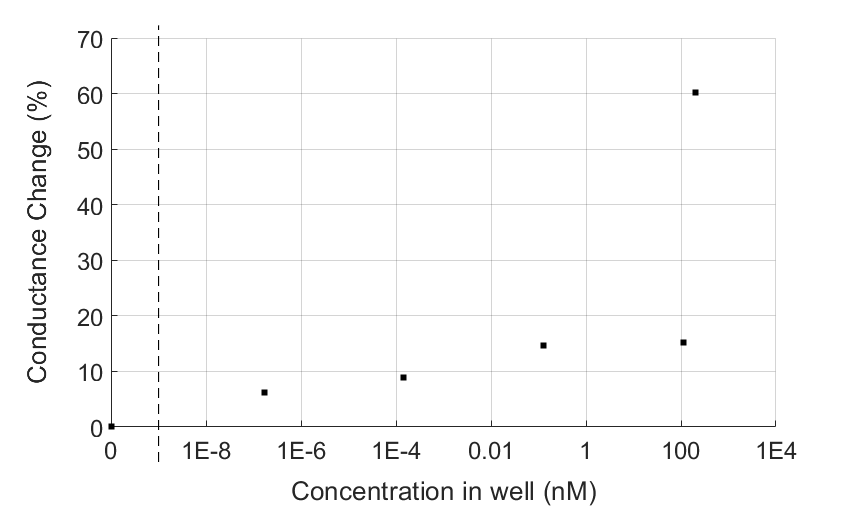
\includegraphics[width=0.8\textwidth,height=\textheight]{figures/ch7/concentrations.png}

}

\caption{\label{fig-EtHex-responses}Cumulative device response
corresponding to the 20 µL analyte additions relative to the ethyl
hexanoate (EtHex) concentration present in the device liquid-gate.}

\end{figure}

However, the final addition resulted in an unexpectedly large response
of \(\sim\) 45\% which dramatically deviates from this well-established
trend. This large response occurs when the concentration of ethyl
hexanoate in the well is approximately doubled from \(\sim\) 100 nM to
\(\sim\) 200 nM. The size of this response well exceeds any error due to
insufficient mixing in the PDMS, which is usually on the scale of
\(\sim\) 1\% (\textbf{?@sec-salt-conc-series}). The analysis in the
subsequent section (Section~\ref{sec-variability}) demonstrates that
this response cannot be explained as the carbon nanotubes (or nanodiscs)
responding to a relatively large concentration of ethyl hexanoate
directly. No significant changes in gate current occur during the
sensing series (Figure~\ref{fig-EtHex-aqueous-sensing}), so the response
cannot be explained as being due to changes in the gate capacitance due
to leakage current. The responses of OR22a to target analyte at
liquid-gate concentrations above 1 nM have not previously been
investigated for field-effect transistor sensors
\autocite{Murugathas2019a,Murugathas2020}. More research may be required
to understand device behaviour at analyte concentrations well above the
apparent saturation regime at high picomolar concentrations.

\hypertarget{sec-variability}{%
\section{Addressing Biosensor Variability}\label{sec-variability}}

\hypertarget{sec-variability-biosensor}{%
\subsection{Variability in Biosensor
Behaviour}\label{sec-variability-biosensor}}

\begin{figure}

{\centering 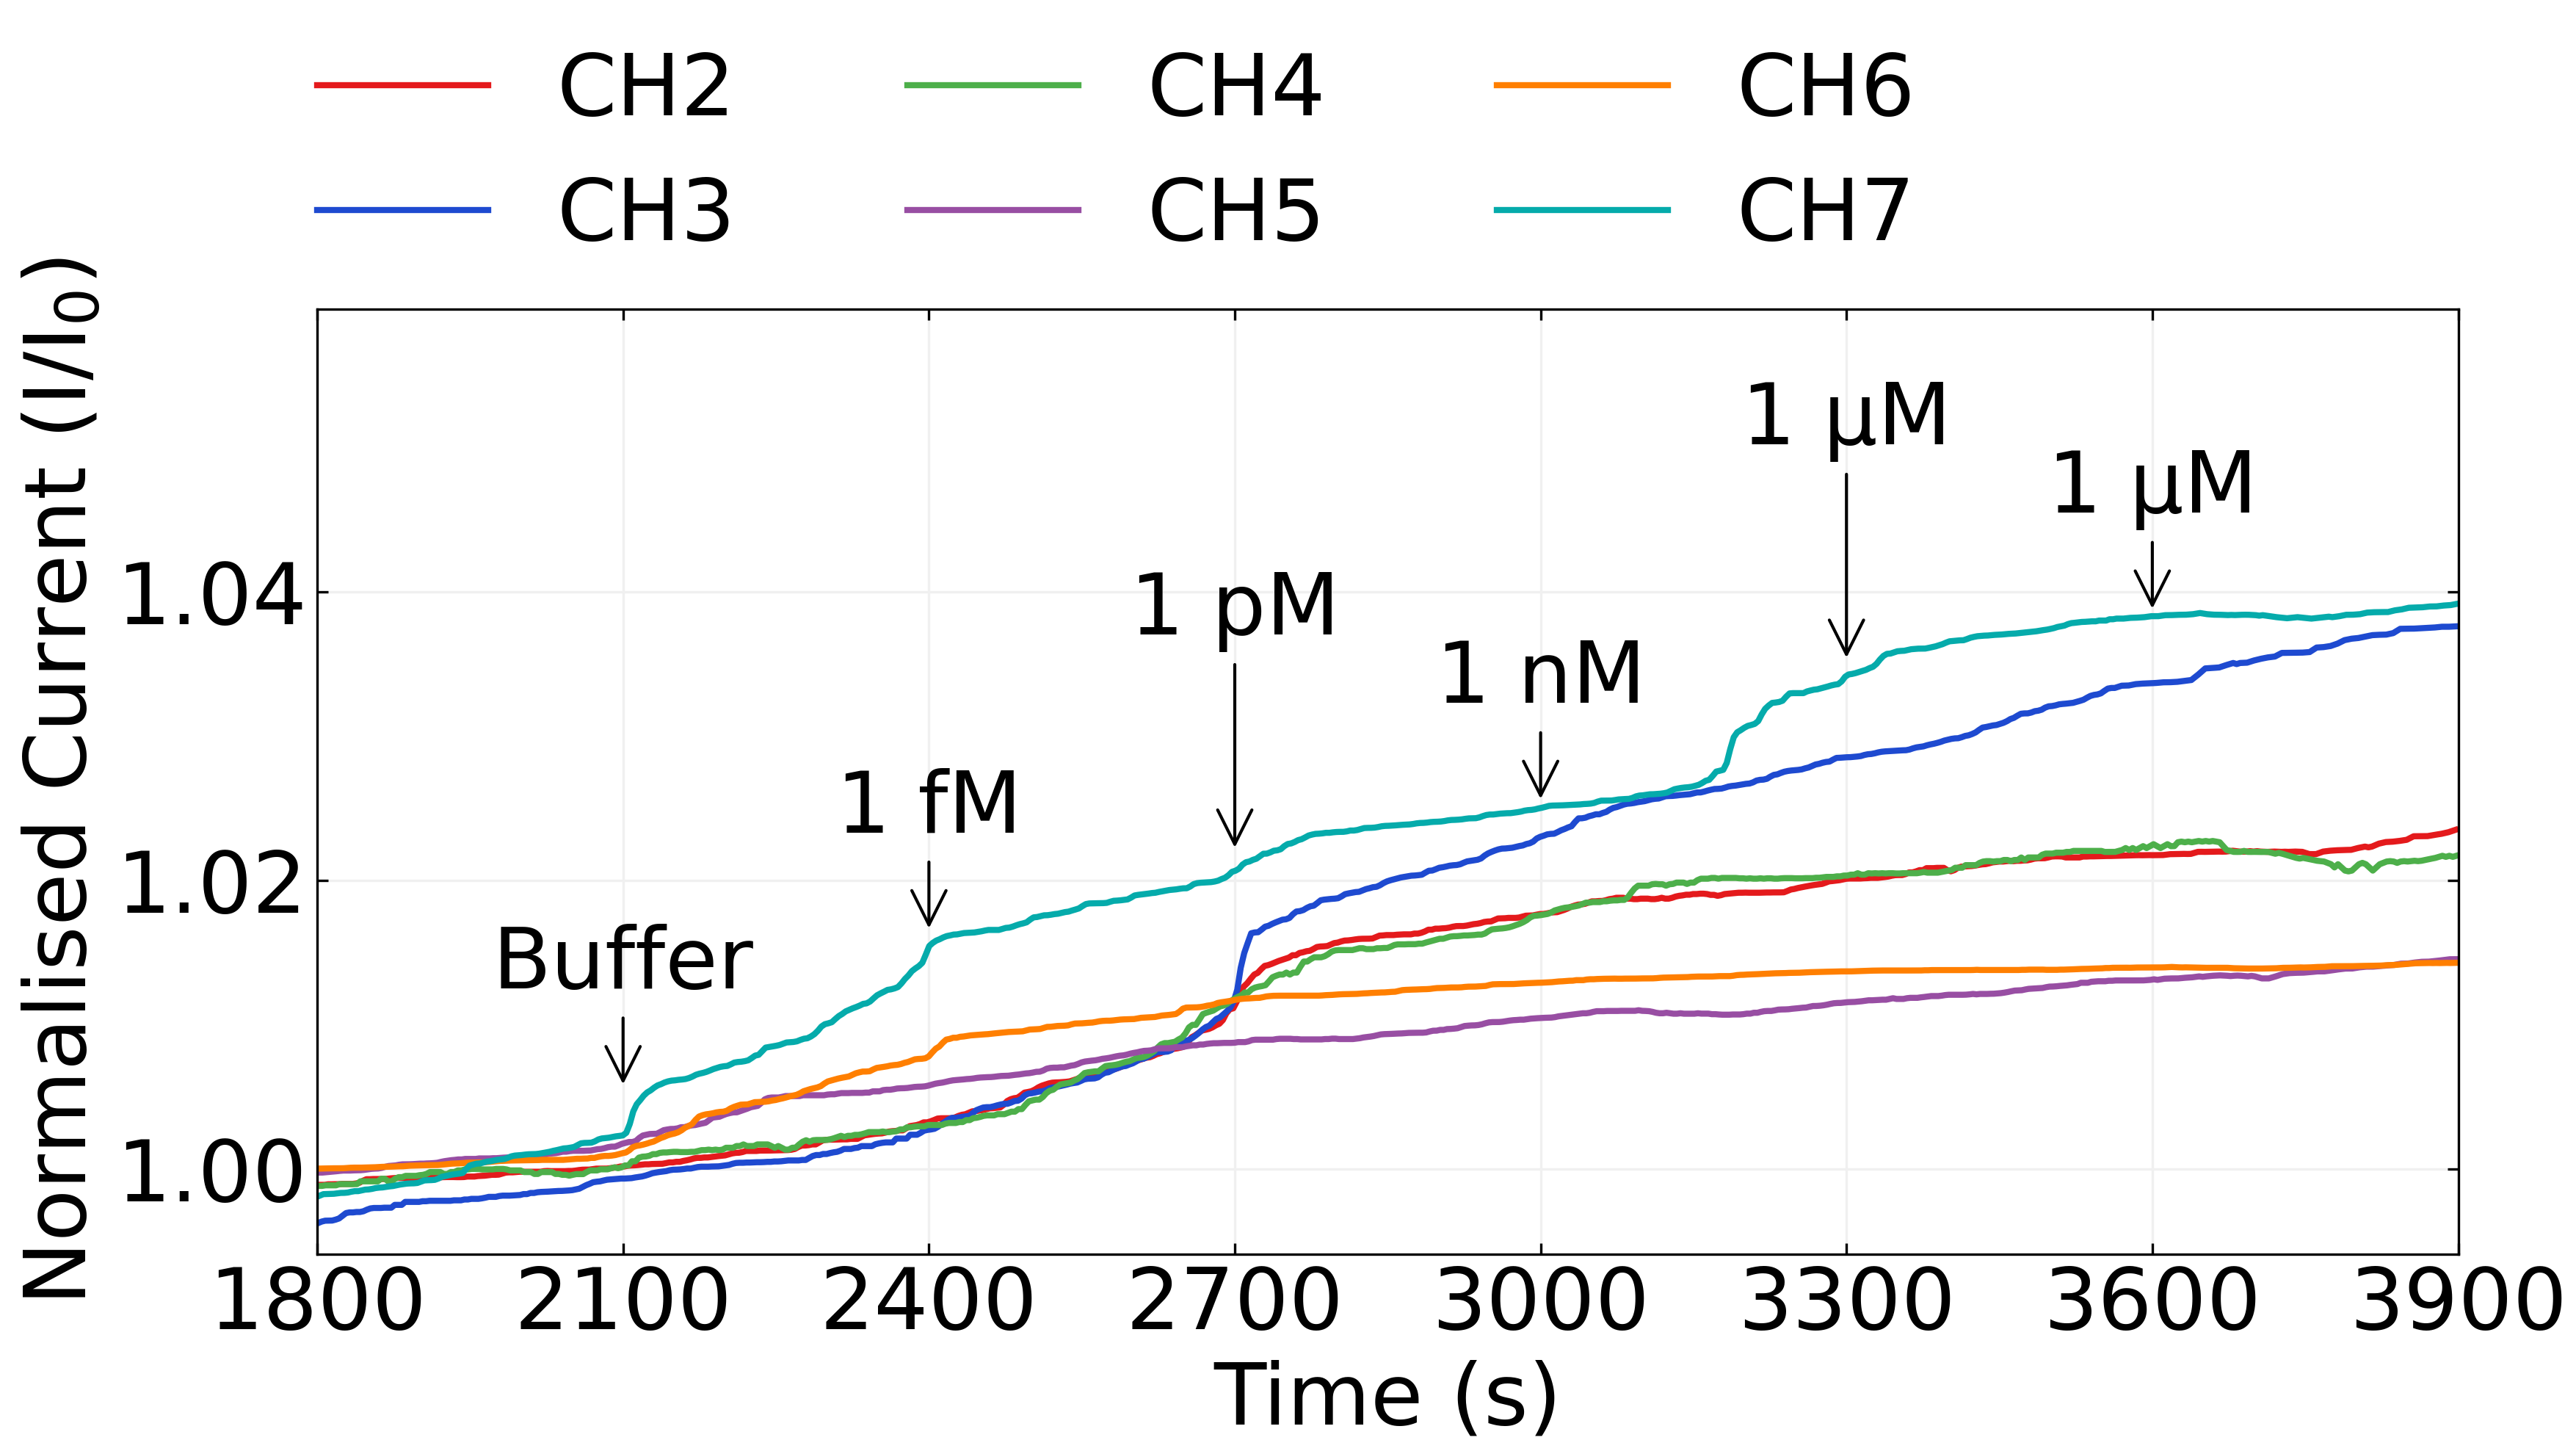
\includegraphics[width=0.7\textwidth,height=\textheight]{figures/ch7/Q4C4_OR22a_Functionalised_filtered_detrend_trunc_arrows_normalised.png}

}

\caption{\label{fig-OR22a-variability}The normalised sensing series of
another OR22a-functionalised device across six multiplexed channels,
where current data has been despiked, baseline drift removed and a
moving median filter applied. The concentration of each 20 µL addition
is indicated above the time of addition.}

\end{figure}

Despite the successful detection of ethyl hexanoate by an OR22a
nanodisc-functionalised biosensor in
Section~\ref{sec-aqueous-sensing-EtHex}, it was found that this
behaviour was not readily reproducible. The results from the previous
section were not repeated when using the same procedure for fabrication
of devices alongside an identical functionalisation process with the
same batch of OR22a nanodiscs (ND-OR22a-SB018). The ethyl hexanoate
sensing sequence from six functionalised device channels is shown in
Figure~\ref{fig-OR22a-variability}. The current response to each analyte
addition is similar to that seen after the initial addition without
ethyl hexanoate present. The largest contributing factor to current
change appears to be drift. Unlike the clear decreases in current
subsequent to ethyl hexanoate additions seen in
Figure~\ref{fig-OR22a-series} (c), no decreases are seen in
Figure~\ref{fig-OR22a-variability} to any ethyl hexanoate solution
addition. It is clear that although the same process has been followed
here as in Section~\ref{sec-EtHex-aqueous-sensing}, the functionalised
device is not responding to the presence of target analyte. The device
characteristics were therefore investigated for differences from the
functionalisation results seen in
Section~\ref{sec-working-PBASE-functionalisation}.

Liquid-gated electrical characteristics were taken of each sensing
channel from this device before and after functionalisation with OR22a
nanodiscs, in the same manner as in
Section~\ref{sec-working-PBASE-functionalisation}. These characteristics
are shown in Figure~\ref{fig-OR22a-variability-TX}. The average
threshold shift was \(-0.06 \pm 0.02\), the same as that of a device
functionalised with PBASE in methanol without subsequent
functionalisation with OR22a nanodiscs. To test whether protein was
present on the channel, an atomic force microscope image was taken of
channel 6. The resulting image is shown in
Figure~\ref{fig-OR22a-variability-AFM-comparison} (a) with the mean
substrate height (\(\sim\) 2 nm) masked in green. A binary
representation of the image was also prepared with a 12 nm threshold,
shown in Figure~\ref{fig-OR22a-variability-AFM-comparison} (c). As in
Figure~\ref{fig-working-OR22a-AFM} (f), the surface is densely populated
with non-nanotube features over 50 nm across. These features also form
clusters across the network. Nanodisc agglomerates \(\sim\) 29 \(-\) 37
nm in height are therefore present on channel 6 (following the
discussion in Section~\ref{sec-working-PBASE-functionalisation}),
despite the lack of a significant threshold shift subsequent to
functionalisation. The agglomerates are still relatively small compared
to those reported by Murugathas \emph{et al.}, so the large size of
nanodiscs in Figure~\ref{fig-OR22a-variability-AFM-comparison} relative
to those in Section~\ref{sec-working-PBASE-functionalisation} is
unlikely to be an issue \autocite{Murugathas2019a}.

\begin{figure}

\begin{minipage}[t]{0.03\linewidth}

{\centering 

\raisebox{-\height}{


\includegraphics{figures/(a).png}

}

}

\end{minipage}%
%
\begin{minipage}[t]{0.01\linewidth}

{\centering 

~

}

\end{minipage}%
%
\begin{minipage}[t]{0.45\linewidth}

{\centering 

\raisebox{-\height}{

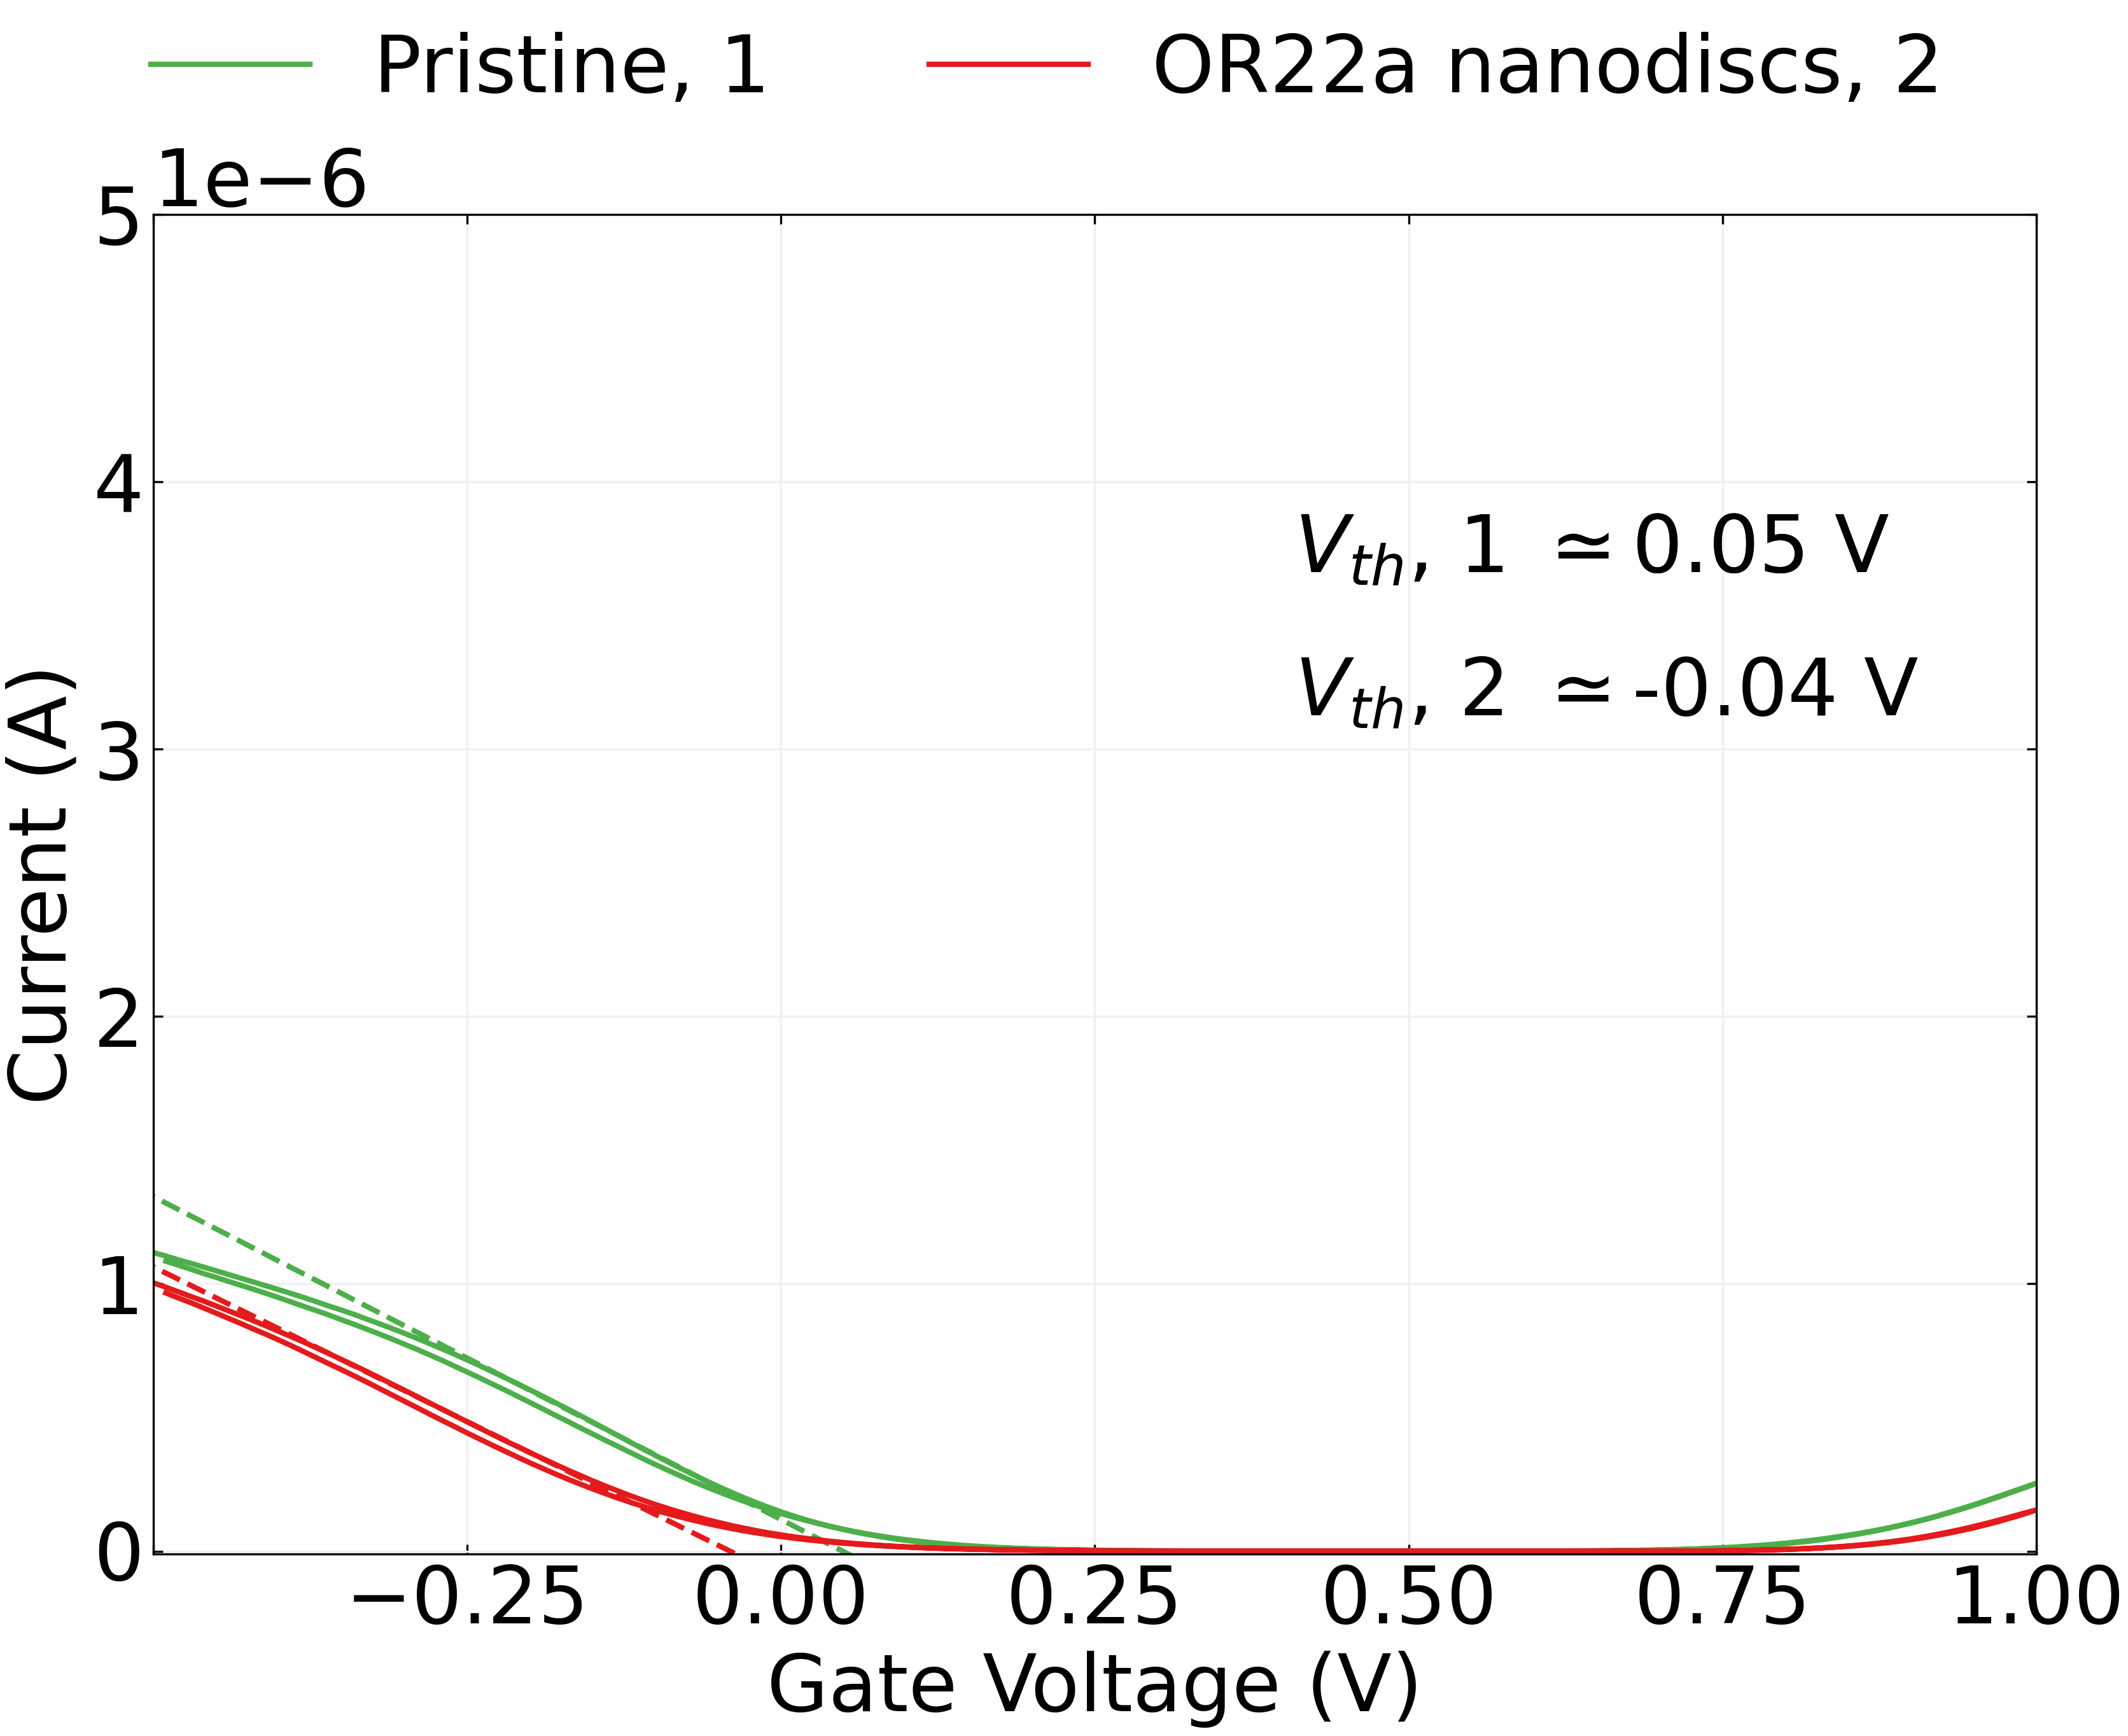
\includegraphics{figures/ch7/Q4C4_ch2.png}

}

}

\end{minipage}%
%
\begin{minipage}[t]{0.01\linewidth}

{\centering 

~

}

\end{minipage}%
%
\begin{minipage}[t]{0.03\linewidth}

{\centering 

\raisebox{-\height}{


\includegraphics{figures/(b).png}

}

}

\end{minipage}%
%
\begin{minipage}[t]{0.01\linewidth}

{\centering 

~

}

\end{minipage}%
%
\begin{minipage}[t]{0.45\linewidth}

{\centering 

\raisebox{-\height}{

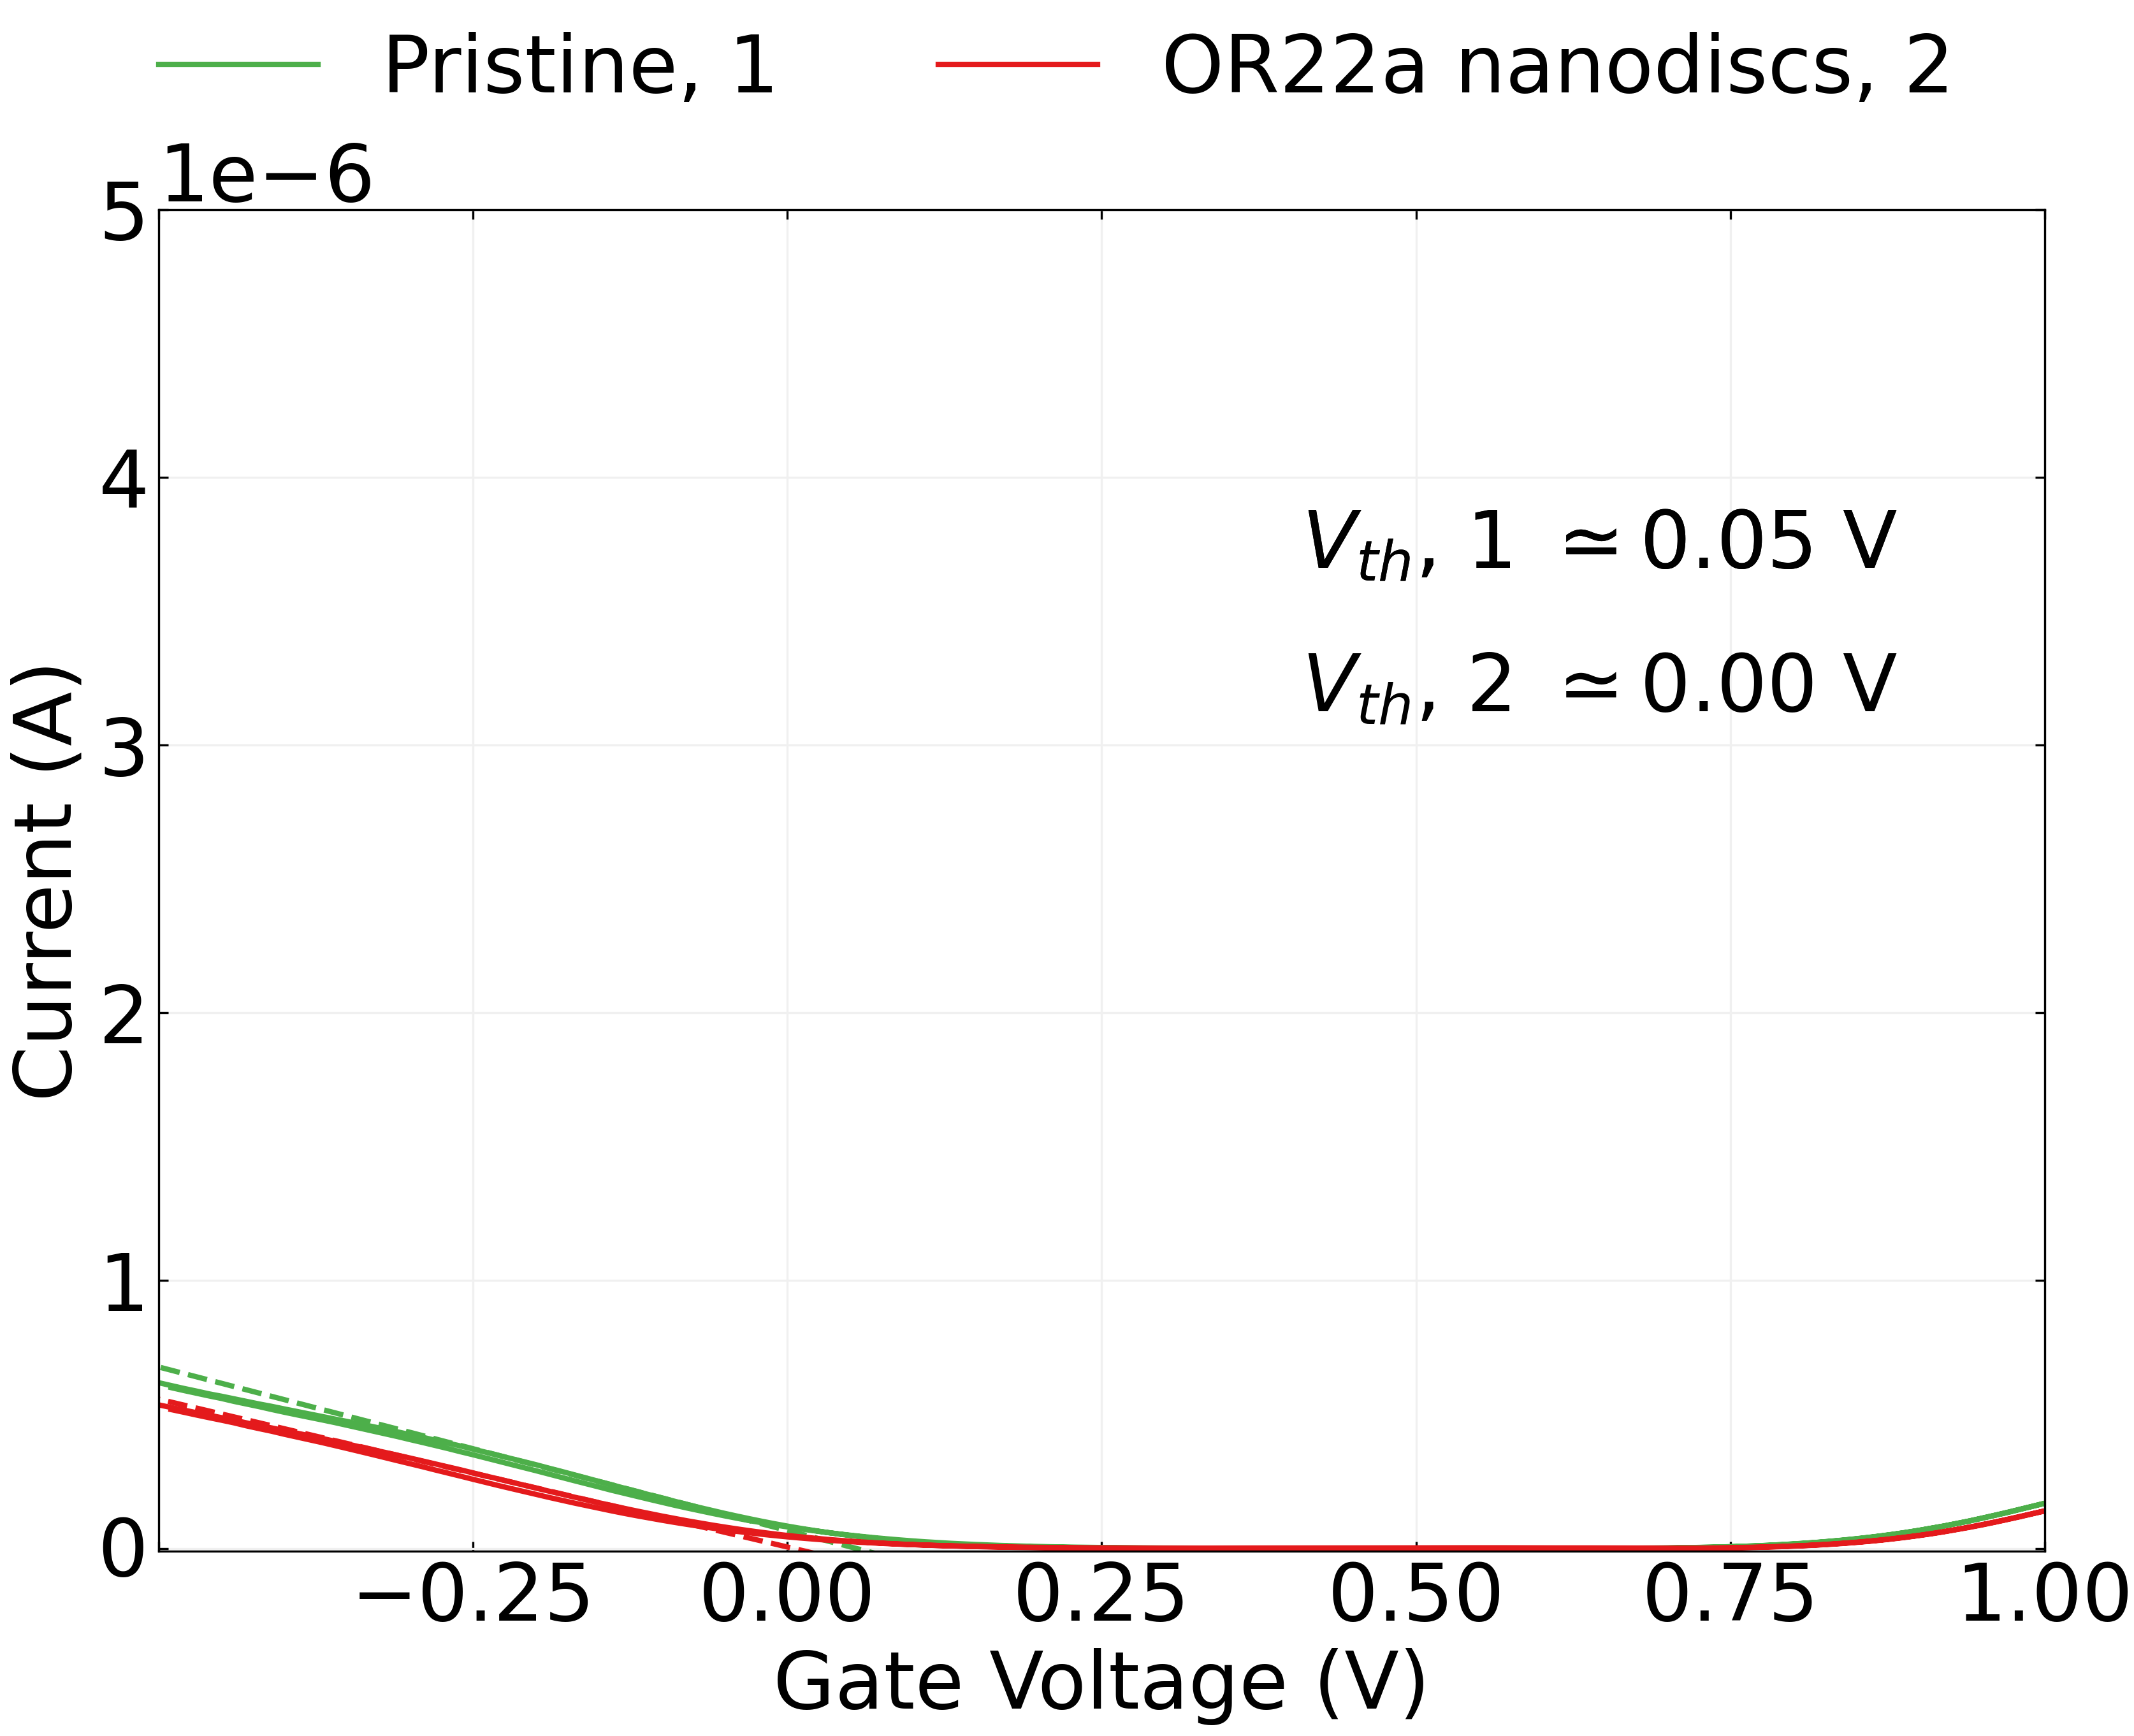
\includegraphics{figures/ch7/Q4C4_ch3.png}

}

}

\end{minipage}%
%
\begin{minipage}[t]{0.01\linewidth}

{\centering 

~

}

\end{minipage}%
\newline
\begin{minipage}[t]{0.03\linewidth}

{\centering 

\raisebox{-\height}{


\includegraphics{figures/(c).png}

}

}

\end{minipage}%
%
\begin{minipage}[t]{0.01\linewidth}

{\centering 

~

}

\end{minipage}%
%
\begin{minipage}[t]{0.45\linewidth}

{\centering 

\raisebox{-\height}{

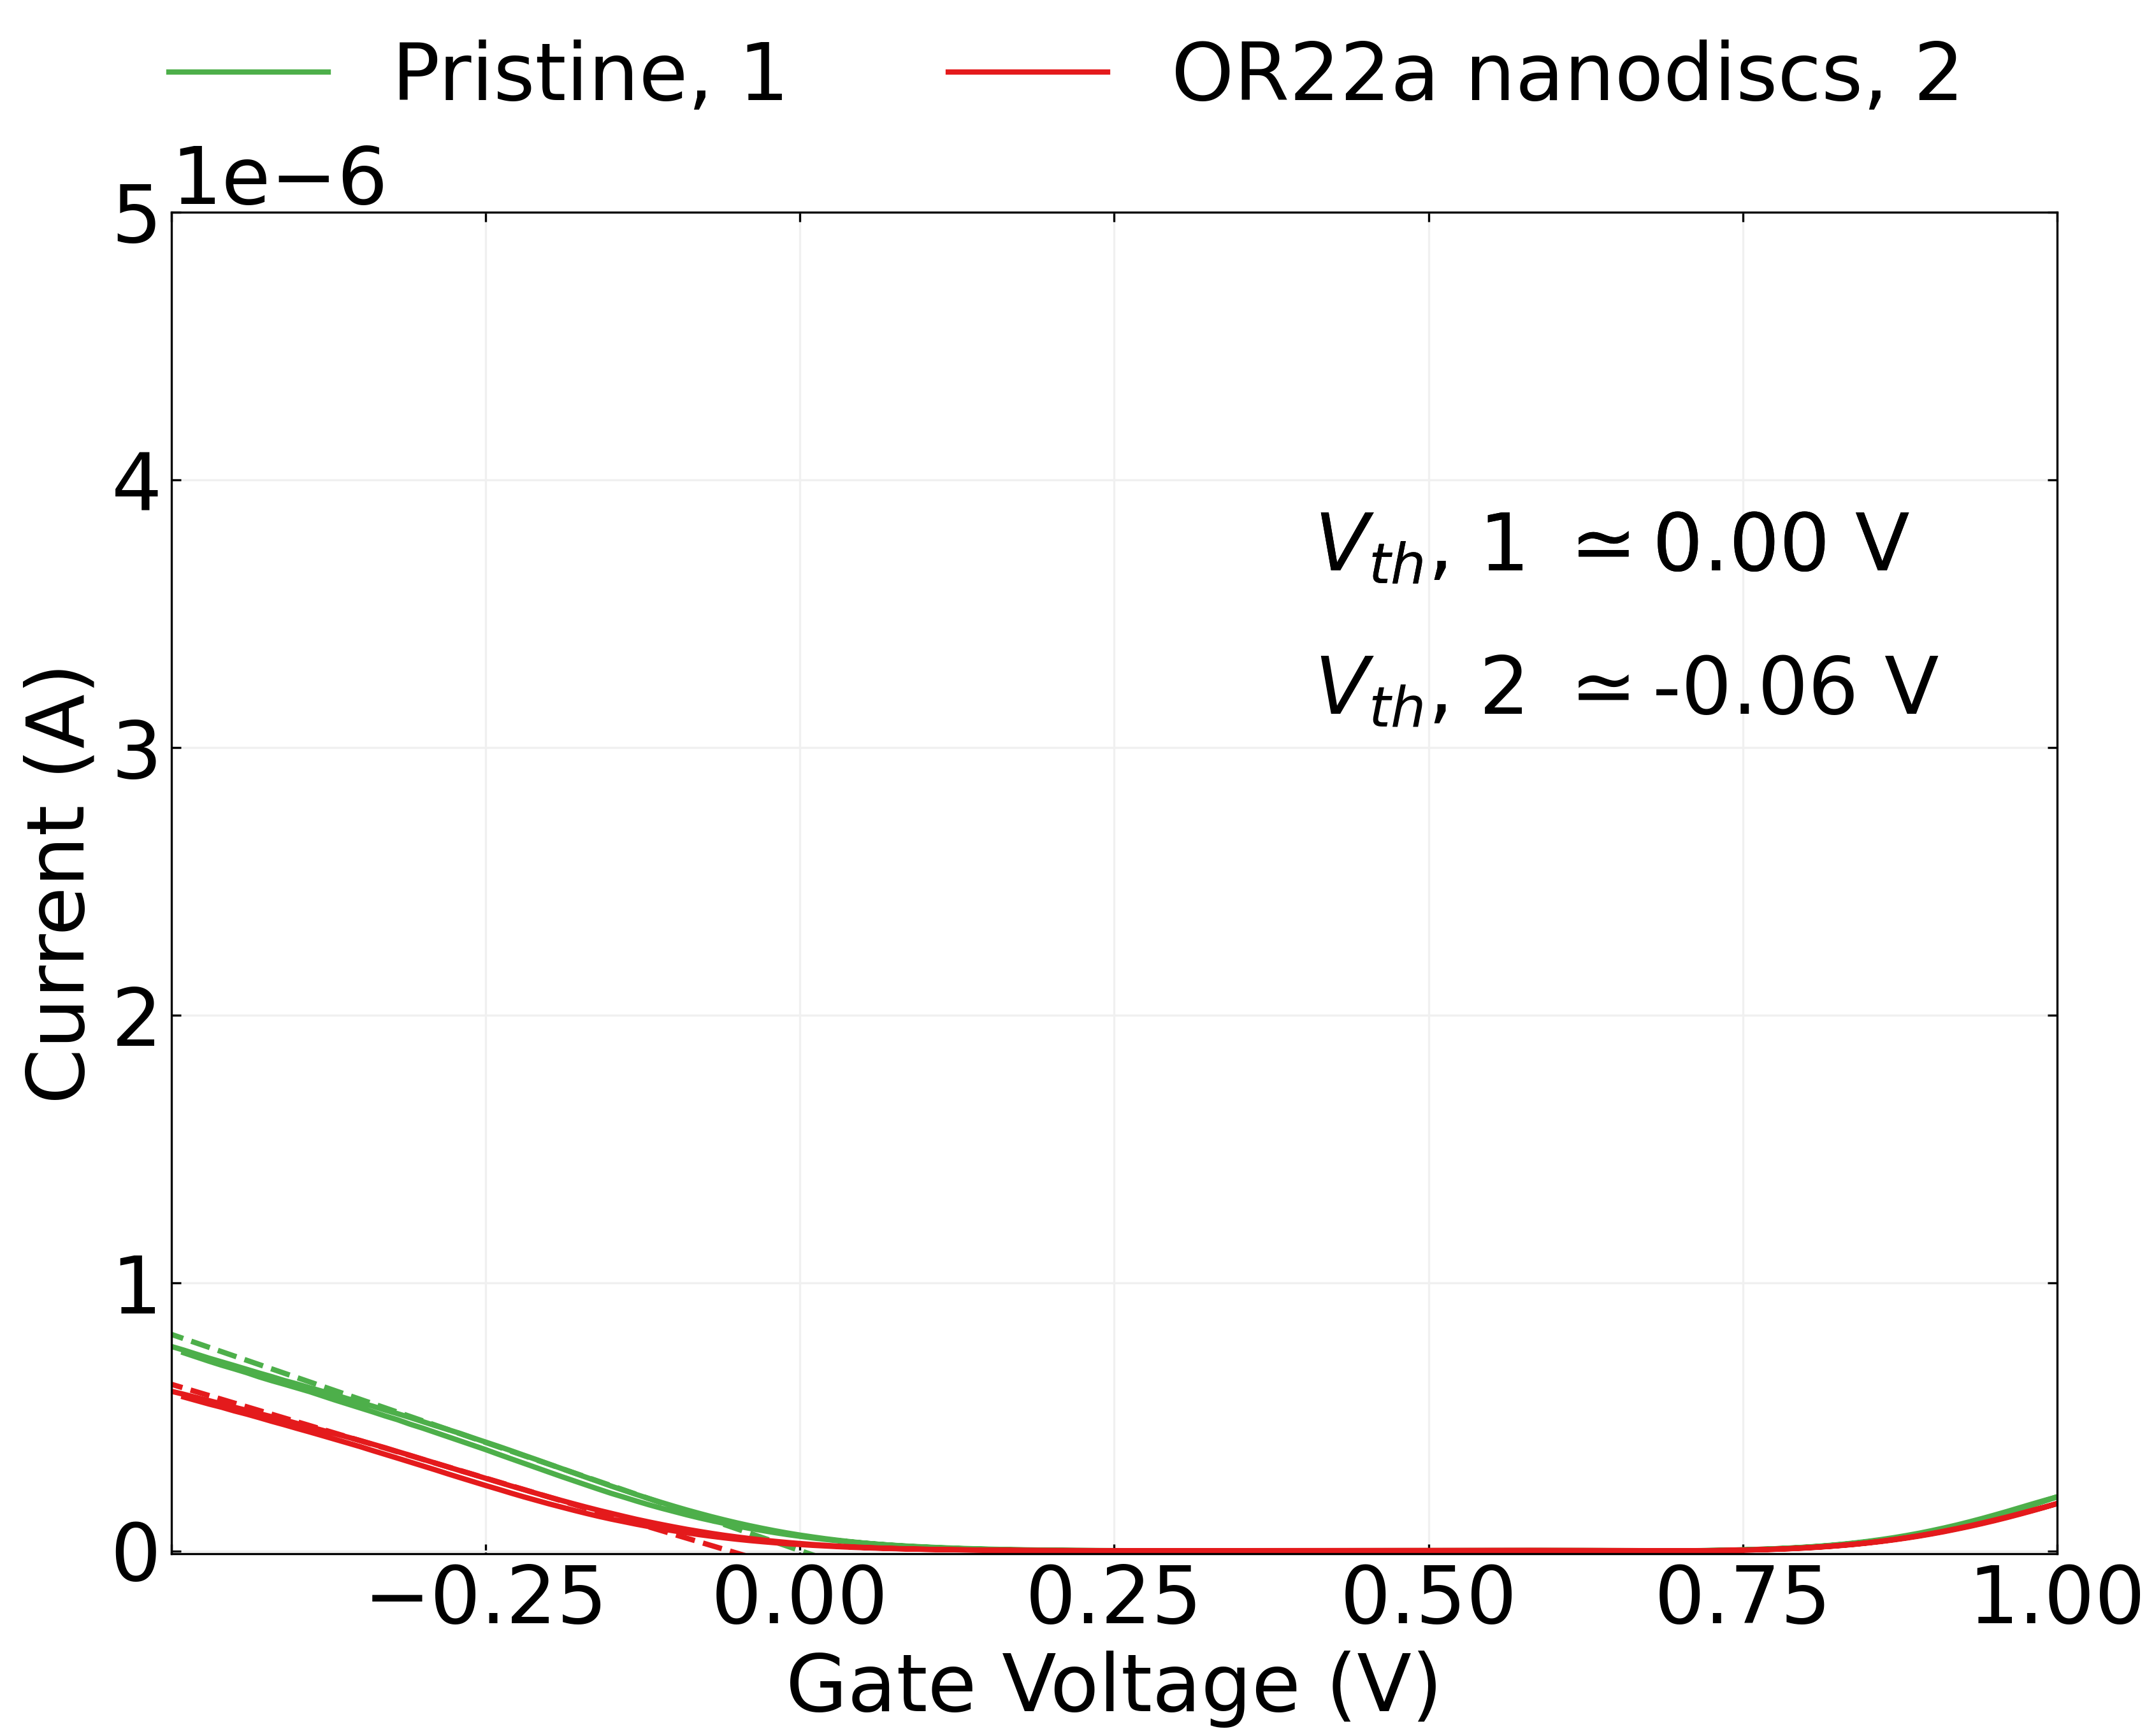
\includegraphics{figures/ch7/Q4C4_ch4.png}

}

}

\end{minipage}%
%
\begin{minipage}[t]{0.01\linewidth}

{\centering 

~

}

\end{minipage}%
%
\begin{minipage}[t]{0.03\linewidth}

{\centering 

\raisebox{-\height}{


\includegraphics{figures/(d).png}

}

}

\end{minipage}%
%
\begin{minipage}[t]{0.01\linewidth}

{\centering 

~

}

\end{minipage}%
%
\begin{minipage}[t]{0.45\linewidth}

{\centering 

\raisebox{-\height}{

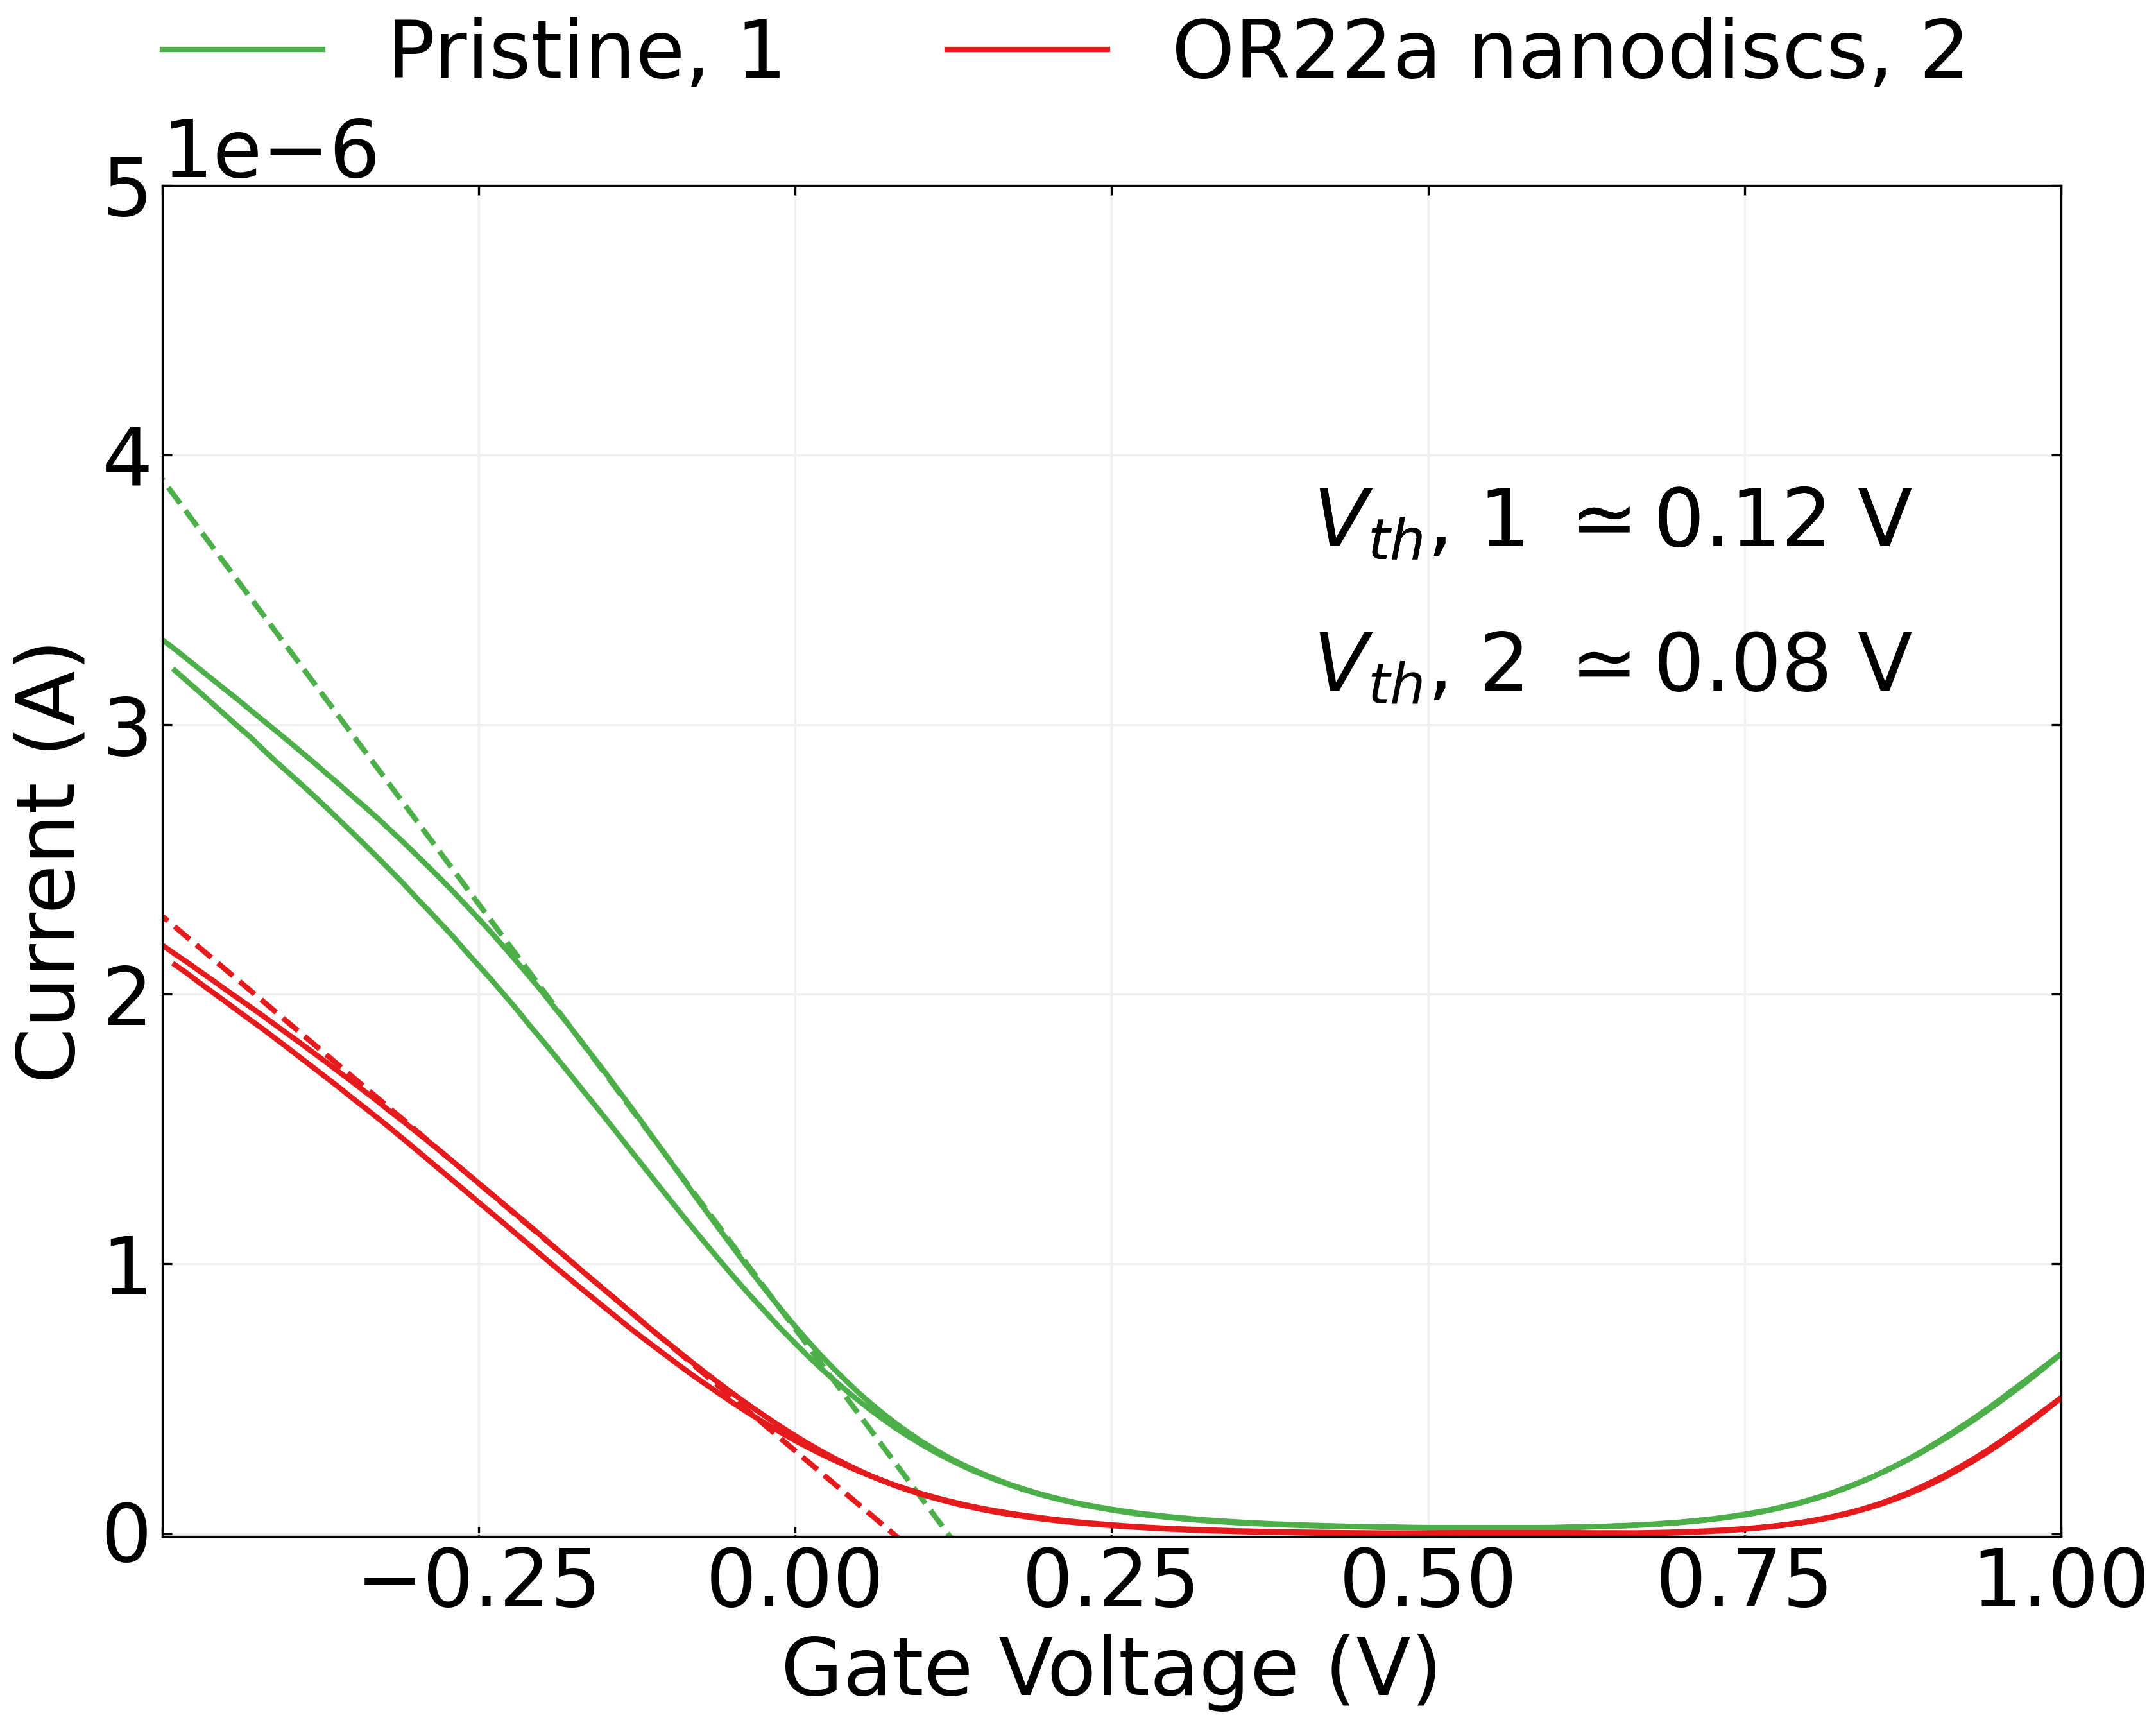
\includegraphics{figures/ch7/Q4C4_ch5.png}

}

}

\end{minipage}%
%
\begin{minipage}[t]{0.01\linewidth}

{\centering 

~

}

\end{minipage}%
\newline
\begin{minipage}[t]{0.03\linewidth}

{\centering 

\raisebox{-\height}{


\includegraphics{figures/(e).png}

}

}

\end{minipage}%
%
\begin{minipage}[t]{0.01\linewidth}

{\centering 

~

}

\end{minipage}%
%
\begin{minipage}[t]{0.45\linewidth}

{\centering 

\raisebox{-\height}{

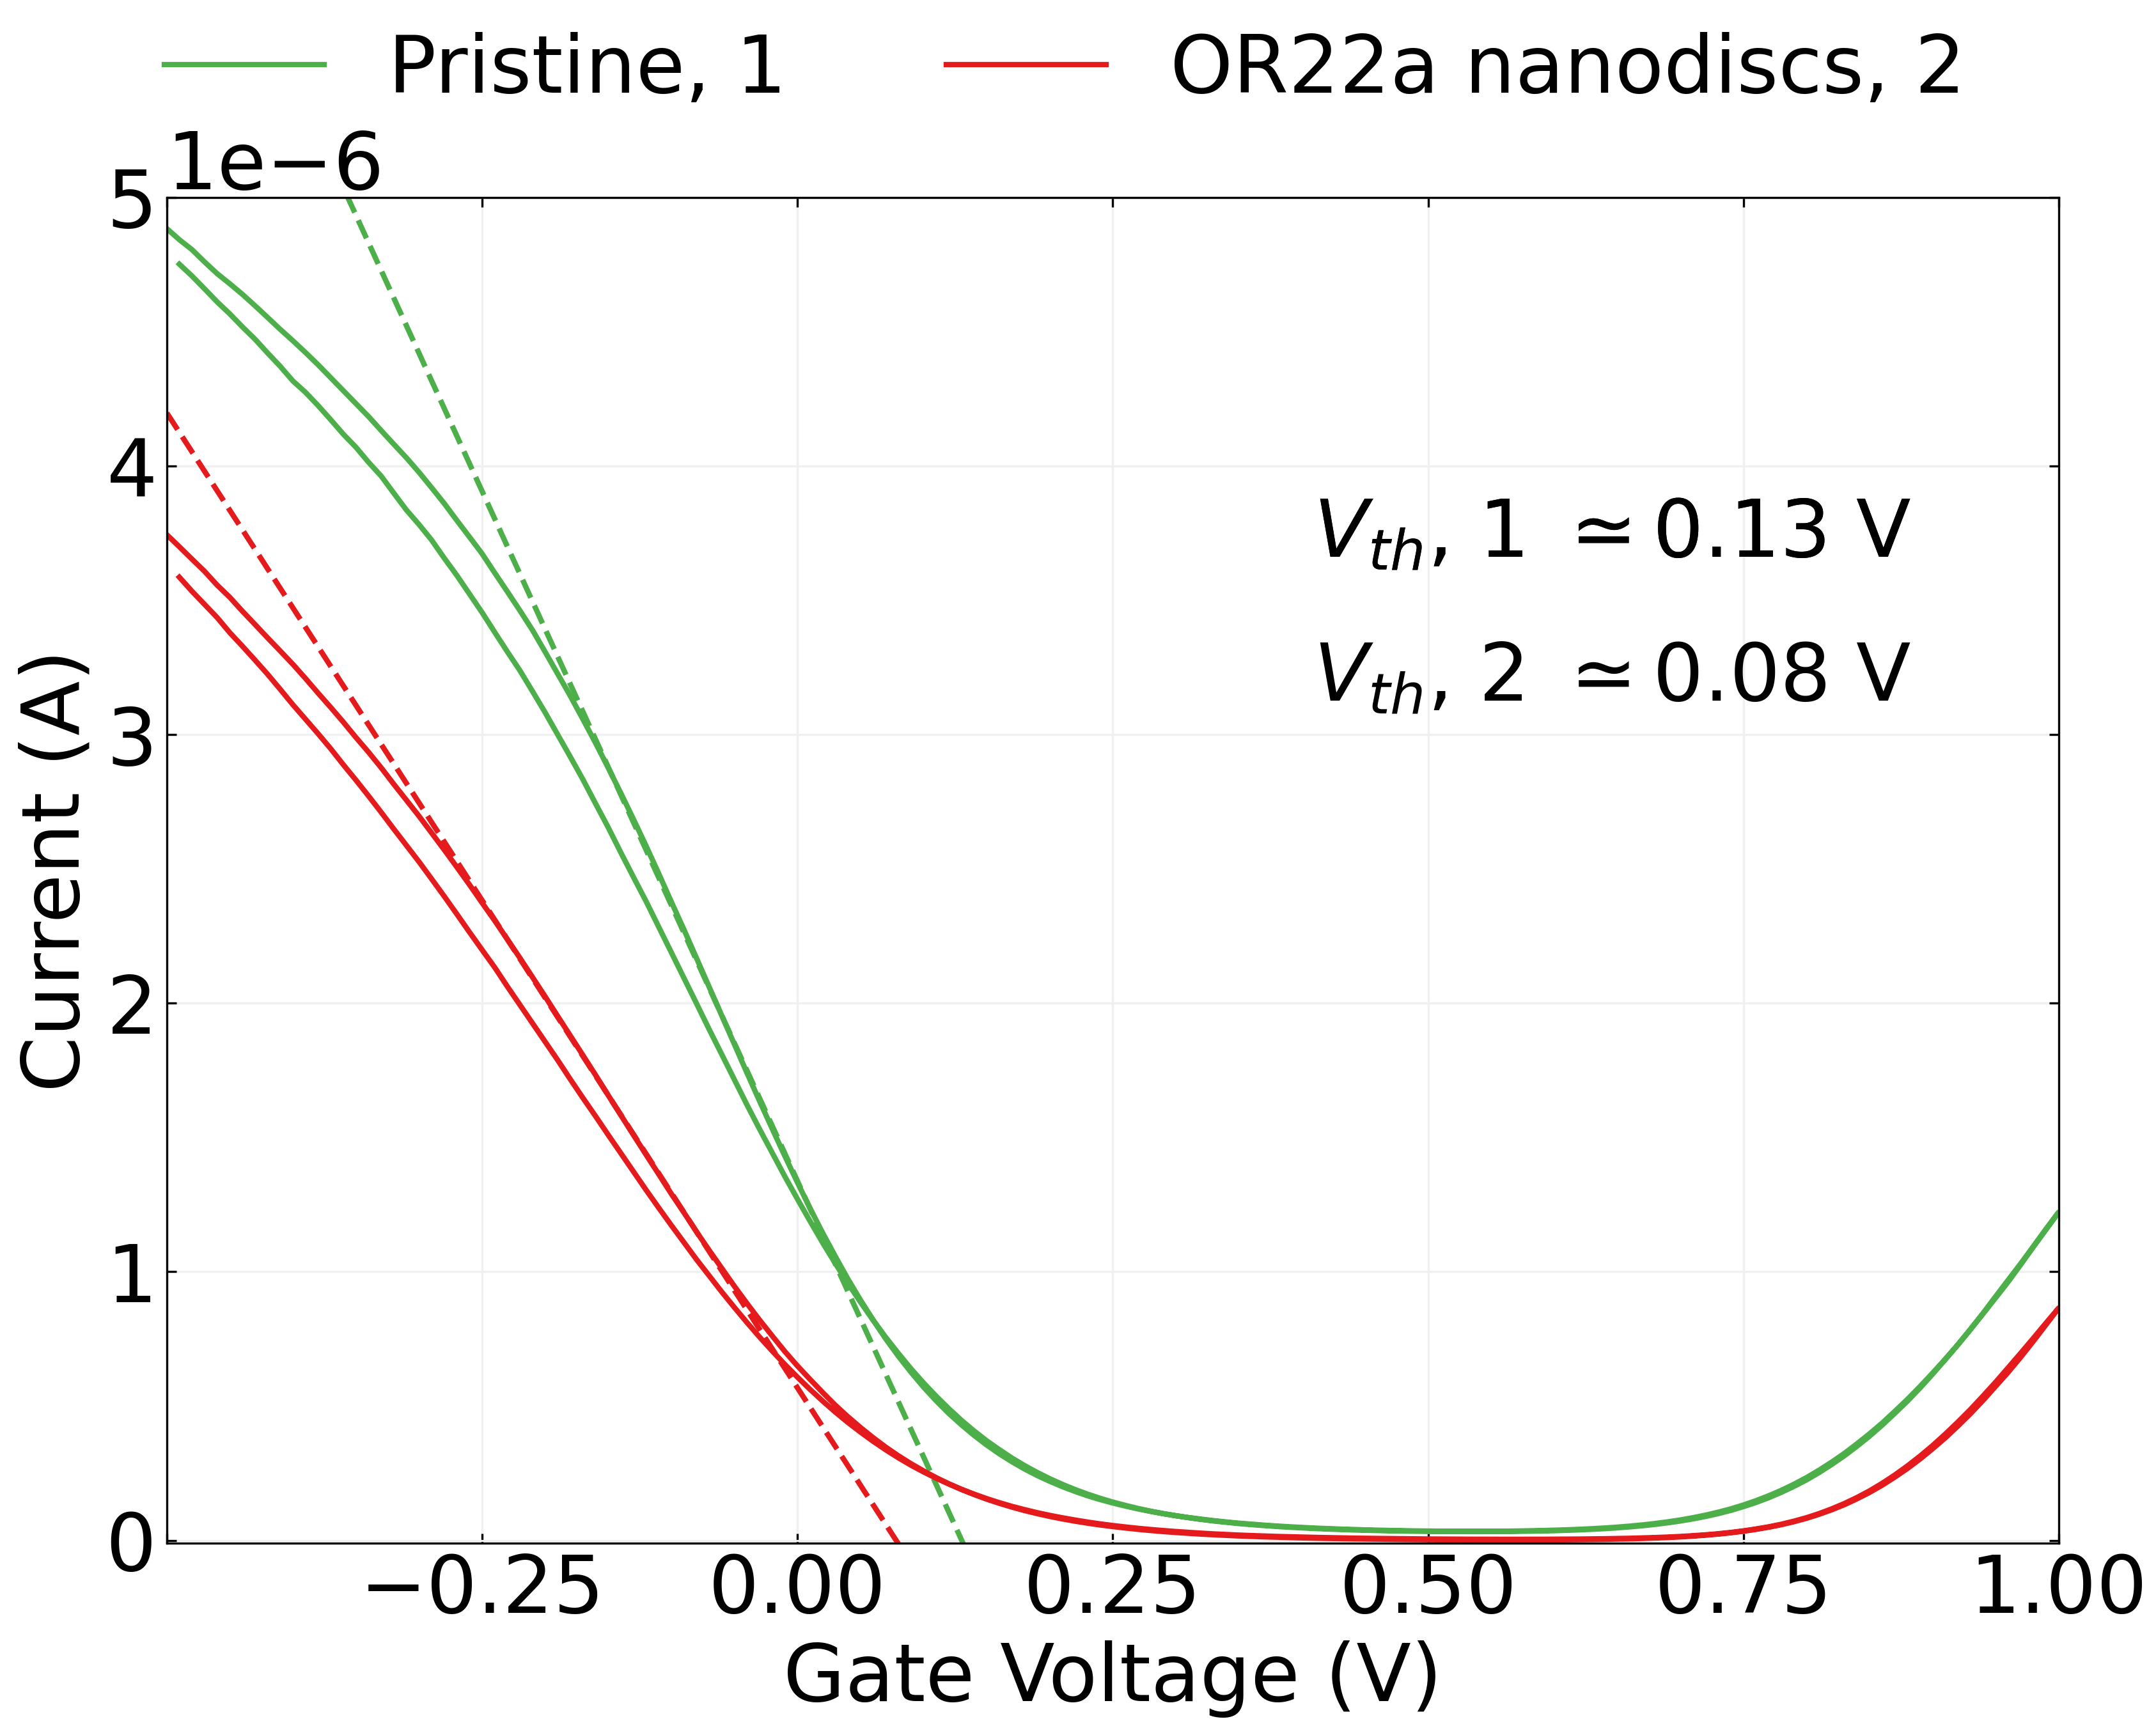
\includegraphics{figures/ch7/Q4C4_ch6.png}

}

}

\end{minipage}%
%
\begin{minipage}[t]{0.01\linewidth}

{\centering 

~

}

\end{minipage}%
%
\begin{minipage}[t]{0.03\linewidth}

{\centering 

\raisebox{-\height}{


\includegraphics{figures/(f).png}

}

}

\end{minipage}%
%
\begin{minipage}[t]{0.01\linewidth}

{\centering 

~

}

\end{minipage}%
%
\begin{minipage}[t]{0.45\linewidth}

{\centering 

\raisebox{-\height}{

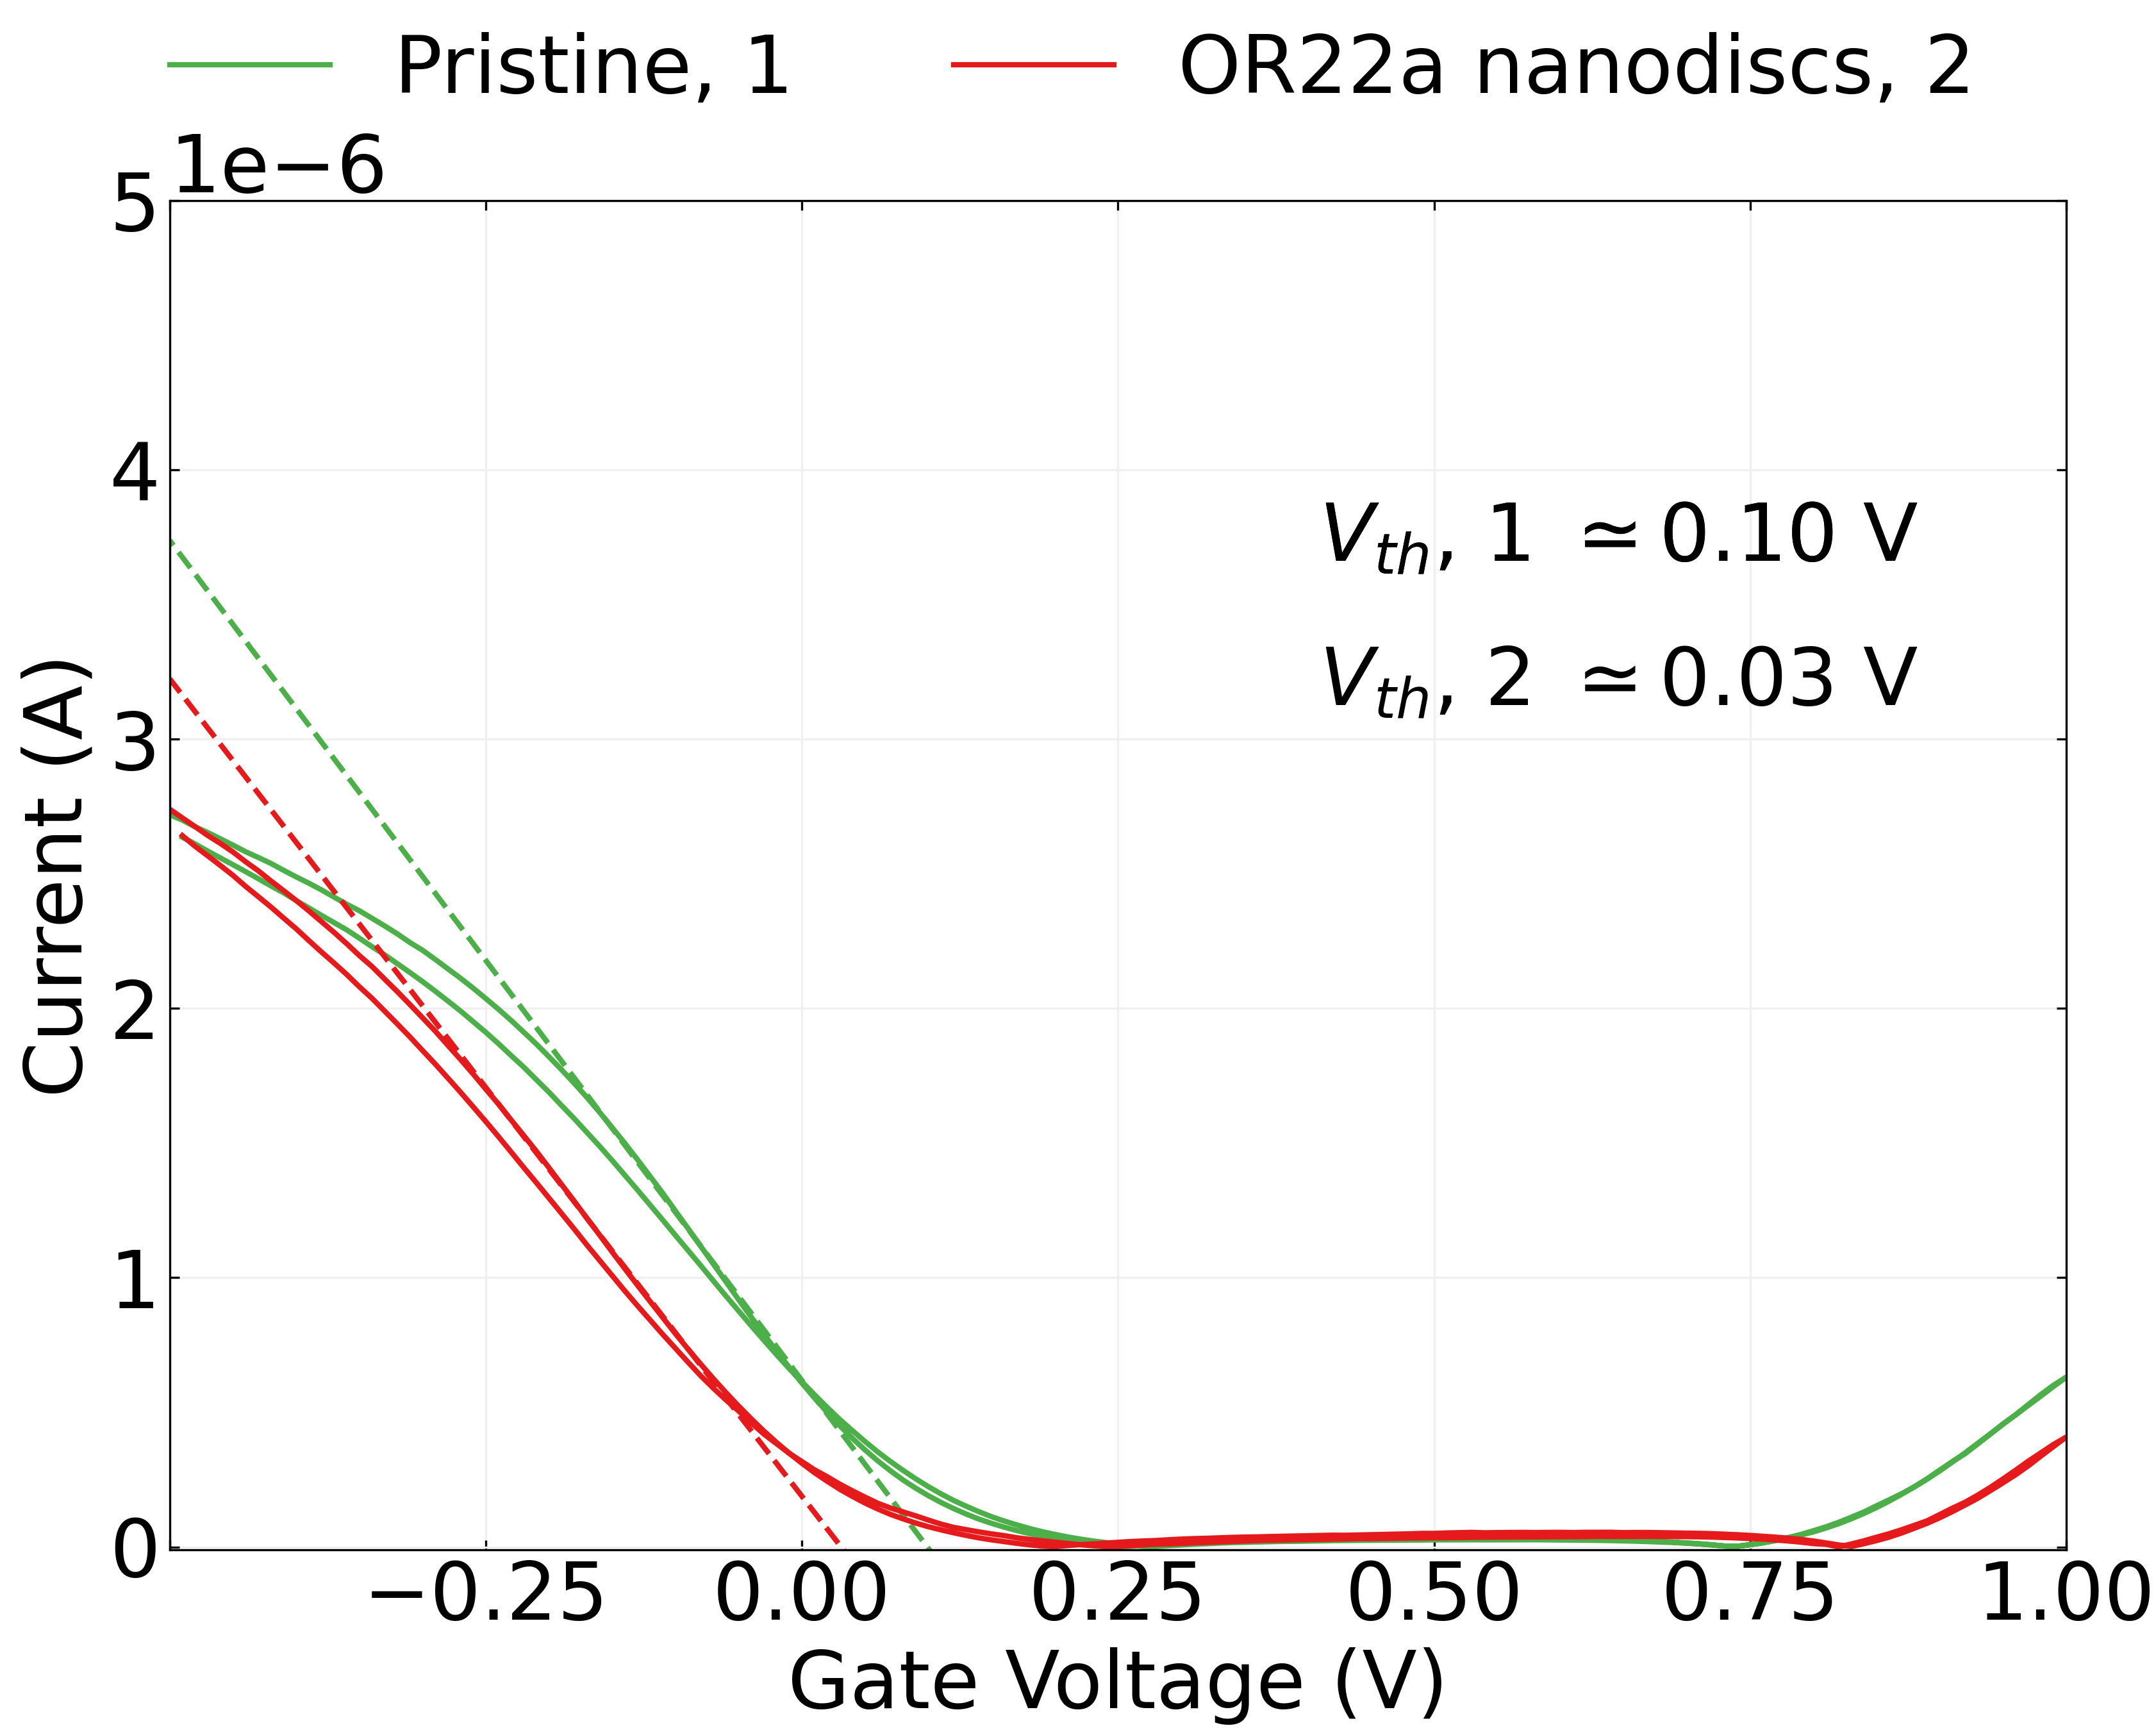
\includegraphics{figures/ch7/Q4C4_ch7.png}

}

}

\end{minipage}%
%
\begin{minipage}[t]{0.01\linewidth}

{\centering 

~

}

\end{minipage}%

\caption{\label{fig-OR22a-variability-TX}Liquid-gated carbon nanotube
network device transfer characteristics before and after OR22a nanodisc
functionalisation. Source-drain voltage was \(V_{ds}\) = 100 mV for both
the forward and reverse sweep. Each subfigure (a)-(f) corresponds to a
different channel of the functionalised device; (a) corresponds to
channel 2, (b) corresponds to channel 3, (c) corresponds to channel 4,
(d) corresponds to channel 5, (e) corresponds to channel 6 and (f)
corresponds to channel 7. The dashed line shown is tangent to the
subthreshold slope of the characteristic curve in the forward direction.
The threshold voltage corresponding to the intercept of this slope with
the x-axis is shown for each transfer characteristic curve.}

\end{figure}

\begin{figure}

\begin{minipage}[t]{0.03\linewidth}

{\centering 

\raisebox{-\height}{

\includegraphics{figures/(a).png}

}

}

\end{minipage}%
%
\begin{minipage}[t]{0.01\linewidth}

{\centering 

~

}

\end{minipage}%
%
\begin{minipage}[t]{0.45\linewidth}

{\centering 

\raisebox{-\height}{

\includegraphics{figures/ch7/Q4C4_CH6_PostSensing_OR22a_Func_AFM100670_00693_mask.png}

}

}

\end{minipage}%
%
\begin{minipage}[t]{0.01\linewidth}

{\centering 

~

}

\end{minipage}%
%
\begin{minipage}[t]{0.03\linewidth}

{\centering 

\raisebox{-\height}{

\includegraphics{figures/(b).png}

}

}

\end{minipage}%
%
\begin{minipage}[t]{0.01\linewidth}

{\centering 

~

}

\end{minipage}%
%
\begin{minipage}[t]{0.45\linewidth}

{\centering 

\raisebox{-\height}{

\includegraphics{figures/ch7/Ned_Q16D2_W4_OR22a1_noPBASE_sensing_2.5micron_256px_00462_2021092_mask.png}

}

}

\end{minipage}%
%
\begin{minipage}[t]{0.01\linewidth}

{\centering 

~

}

\end{minipage}%
\newline
\begin{minipage}[t]{0.03\linewidth}

{\centering 

\raisebox{-\height}{

\includegraphics{figures/(c).png}

}

}

\end{minipage}%
%
\begin{minipage}[t]{0.01\linewidth}

{\centering 

~

}

\end{minipage}%
%
\begin{minipage}[t]{0.45\linewidth}

{\centering 

\raisebox{-\height}{

\includegraphics{figures/ch7/Q4C4_CH6_PostSensing_OR22a_Func_AFM100670_00693_threshold.png}

}

}

\end{minipage}%
%
\begin{minipage}[t]{0.01\linewidth}

{\centering 

~

}

\end{minipage}%
%
\begin{minipage}[t]{0.03\linewidth}

{\centering 

\raisebox{-\height}{

\includegraphics{figures/(d).png}

}

}

\end{minipage}%
%
\begin{minipage}[t]{0.01\linewidth}

{\centering 

~

}

\end{minipage}%
%
\begin{minipage}[t]{0.45\linewidth}

{\centering 

\raisebox{-\height}{

\includegraphics{figures/ch7/Ned_Q16D2_W4_OR22a1_noPBASE_sensing_2.5micron_256px_00462_2021092_threshold.png}

}

}

\end{minipage}%
%
\begin{minipage}[t]{0.01\linewidth}

{\centering 

~

}

\end{minipage}%

\caption{\label{fig-OR22a-variability-AFM-comparison}An scaled atomic
force microscope image of channel 6 from the unresponsive device is
shown in (a). An atomic force microscope image of a device modified with
OR22a nanodiscs without the use of PBASE is shown in (b), with an
imaging artifact bounded in red. A binary representation of the atomic
force microscope image in (a) with a threshold height of 12 nm is shown
in (c); a binary representation of the atomic force microscope image in
(b) is shown in (d), with a threshold height of 14 nm. In (a) and (b),
the average substrate height has been highlighted green with the
Gwyddion software mask tool.}

\end{figure}

Both OR nanodisc and empty nanodisc attachment via PBASE have been shown
to cause significant gating of the network
(Section~\ref{sec-working-PBASE-functionalisation}). The amine group on
proteins can be attached directly onto carbon nanotubes by adsorption,
although this attachment is relatively weak \autocite{Bradley2004}.
Figure~\ref{fig-OR22a-variability-AFM-comparison} (b) shows an AFM image
of a carbon nanotube network film after submersion in a 10 µL/mL OR22a
nanodisc in PBS solution for 1 hour (batch NDOR22a-0016-1), without
prior exposure to PBASE in methanol. A \(\sim\) 2 nm high image artifact
(see \textbf{?@sec-pristine-AFM}) is present in the lower left of the
image, bounded in red, and so the median substrate height of the image
is found at \(\sim\) 4 nm, highlighted green in
Figure~\ref{fig-OR22a-variability-AFM-comparison} (b). A binary
representation of this AFM at with a threshold height of 14 nm is shown
in Figure~\ref{fig-OR22a-variability-AFM-comparison} (d), where nanodisc
agglomerations are clearly visible. Therefore, it might be reasoned that
the lack of a gating effect even while nanodiscs are present results
from a direct attachment mechanism which circumvents the PBASE linker.

\begin{figure}

\begin{minipage}[t]{0.03\linewidth}

{\centering 

\raisebox{-\height}{

\includegraphics{figures/(a).png}

}

}

\end{minipage}%
%
\begin{minipage}[t]{0.01\linewidth}

{\centering 

~

}

\end{minipage}%
%
\begin{minipage}[t]{0.49\linewidth}

{\centering 

\raisebox{-\height}{

\includegraphics{figures/ch7/Q4C8_filtered_trunc_arrows_normalised.png}

}

}

\end{minipage}%
%
\begin{minipage}[t]{0.03\linewidth}

{\centering 

\raisebox{-\height}{

\includegraphics{figures/(b).png}

}

}

\end{minipage}%
%
\begin{minipage}[t]{0.01\linewidth}

{\centering 

~

}

\end{minipage}%
%
\begin{minipage}[t]{0.42\linewidth}

{\centering 

\raisebox{-\height}{

\includegraphics{figures/ch7/Q4C8_ch4_without_gate_current.png}

}

}

\end{minipage}%
%
\begin{minipage}[t]{0.01\linewidth}

{\centering 

~

}

\end{minipage}%

\caption{\label{fig-OR22a-variability-noPBASE}Real-time sampling using
channel 4 of the device modified with OR22a nanodisc solution without
prior exposure to PBASE or methanol shown in (a). A 20 µL addition of
1\% v/v DMSO \(1 \times\) PBS was made at 200 s. Subsequently, 20 µL
additions of ethyl hexanoate diluted in 1\% v/v DMSO \(1 \times\) PBS
were made at 400 s, 600 s, 800 s and 1000 s and 1200 s, with the
concentration of each addition indicated above the time of addition.
Liquid-gated carbon nanotube network device transfer characteristics of
the same channel are shown in (b), before and after functionalisation.
Source-drain voltage was \(V_{ds}\) = 100 mV.}

\end{figure}

Figure~\ref{fig-OR22a-variability-noPBASE} (a) shows the sensing results
from the device functionalised without the use of PBASE. Small, positive
current responses to additions of ethyl hexanoate diluted in 1\% v/v
DMSO \(1 \times\) PBS are visible. These responses may may result from
the weakly attached OR22a nanodiscs being mechanically removed by the
pressure of each addition on the device channels. While the sensing
response shows similarities with that seen in
Figure~\ref{fig-OR22a-variability}, the electrical characteristics of
the device channel are starkly different to those in
Figure~\ref{fig-OR22a-variability-TX}. These channel characteristics are
shown in Figure~\ref{fig-OR22a-variability-noPBASE} (b). The negative
threshold shift was -0.27 V, far larger than any seen in
Figure~\ref{fig-OR22a-variability-TX} and similar in size to the
threshold shift after functionalisation seen for the working biosensor
in Figure~\ref{fig-OR22a-TX-comparison}. Despite the difference in
attachment mechanism, there is still significant electrical modification
of the channel by the nanodiscs not seen for the unresponsive device in
Figure~\ref{fig-OR22a-variability}. It appears that attachment by
mechanisms other than PBASE cannot sufficiently explain the variability
in sensor behaviour.

A new explanation is therefore required for this apparently
contradictory scenario where nanodiscs can be present on a device
channel without the observation of significant gating effects
post-functionalisation. The most straightforward explanation is that no
reliable correlation exists between the two phenomena. Given the
consistent threshold shift results for various linker functionalisations
seen in \textbf{?@sec-noncovalent-functionalisation}, this scenario
implies a significant variation in protein structure and charge
behaviour within a single nanodisc batch, which seems unlikely. Another
possibility is that some type of surface coating is causing nanodiscs to
not attach to either PBASE or the carbon nanotubes. This surface coating
might be attractive, attaching to both nanodiscs and carbon nanotubes,
but forming a barrier layer between the two. Alternatively, this coating
might be repulsive, causing nanodiscs to attach weakly to the substrate
around the carbon nanotubes and not the nanotubes themselves. Variations
in the degree to which a network is coated may then explain why the same
functionalisation method might work for one device but not another. The
following section investigates ways of eliminating possible sources of
surface coating for more reliable functionalisation results.

\hypertarget{sec-contamination}{%
\subsection{Potential Sources of Variability}\label{sec-contamination}}

Throughout the course of this thesis, multiple potential candidates for
the unwanted surface coating discussed in the previous section have been
identified. These include the surfactant used in carbon nanotube
deposition (\textbf{?@sec-pristine-morphology},
\textbf{?@sec-pristine-electrical-characterisation}), the solvent used
in functionalisation (\textbf{?@sec-PBASE-electrical-characterisation}),
residual photoresist (\textbf{?@sec-photoresist-contamination}), and the
hydrophobic layer which naturally forms on graphene and carbon nanotubes
in air (\textbf{?@sec-hydrophobicity}). Another possibility is that
PBASE itself is acting as a surface coating, which could result from
multilayer coverage restricting access by the odorant receptors to
directly attached PBASE (\textbf{?@sec-PBASE-attachment}).
Alternatively, PBASE may have hydrolysed into PBA prior to attachment,
forming an inert surface layer upon \(\pi\)-stacking around the carbon
nanotubes. However, no threshold shift directly attributable to PBA
attachment should occur (\textbf{?@sec-PBA-characterisation}), and this
is not what was observed when characterising the non-working device in
Section~\ref{sec-variability-biosensor}. To understand which of these
candidates is responsible for the significant variability in biosensor
functionality, the sensing procedure was performed with slight
variations on the biosensor fabrication and functionalisation
procedures. In each test, an individual element of one of these
procedures was altered to prevent the introduction of a specific surface
coating. The biosensor was then characterised and tested to see if it
would respond to its target odorant.

\hypertarget{spurious-responses}{%
\subsubsection*{Spurious Responses}\label{spurious-responses}}
\addcontentsline{toc}{subsubsection}{Spurious Responses}

\begin{figure}

{\centering \includegraphics[width=0.62\textwidth,height=\textheight]{figures/ch7/NGW4_D7_OR22aliposome_sampling_220623_detrend_trunc_arrows_normalised.png}

}

\caption{\label{fig-DMSO-concentration}Response to changing the
concentration of DMSO in the PDMS well of a OR22a-functionalised sensor.
Source-drain voltage was set at \(V_{ds}\) = 100 mV while gate voltage
was set at \(V_g\) = 0 V. The well originally contained 100 µL of 1\%
v/v DMSO 1X PBS. 20 µL additions of DMSO in PBS were made at 3300 s and
3600 s.}

\end{figure}

Before testing to see if a surface coating was responsible for the lack
of response seen to ethyl hexanoate by the device in
Section~\ref{sec-variability-biosensor}, it was important to investigate
the possibility the signals seen in
Section~\ref{sec-EtHex-aqueous-sensing} were false positives. The highly
sensitive device channel could credibly respond to three different rapid
environmental changes occurring with each addition: the mechanical
action of the addition, a difference between the 0.5\% v/v DMSO in
\(1 \times\) PBS containing the analyte and the 0.5\% v/v DMSO in
\(1 \times\) PBS already in the well, or a direct response to analyte.
It is important to eliminate the first two possibilities to be certain
that the device is responding to analyte. The control series as it
stands demonstrates responses cannot be explained by mechanical action.
All analyte solutions are prepared simultaneously using the same
\(1 \times\) PBS, taking care to avoid cross-contamination, so responses
are unlikely to result from a difference between the \(1 \times\) PBS in
the analyte solution and the \(1 \times\) PBS in the well. It then must
be verified whether a functionalised device channel will respond to a
change in DMSO concentration, which is the result of the DMSO
concentration in an analyte addition being different to the
concentration in the PDMS well.

Figure~\ref{fig-DMSO-concentration} shows that a increase in DMSO
concentration in the well from 1\% v/v to 2.5\% v/v leads to a steep
drop in current of 0.5\% \(-\) 1.5\% across two OR22a-functionalised
device channels, significantly smaller than the \textgreater2\% changes
seen in Section~\ref{sec-EtHex-aqueous-sensing}. Furthermore, as precise
measurements were used during analyte preparation, a change in
proportion of DMSO in the well of this scale during a sensing sequence
is unlikely. It therefore seems improbable that a change in DMSO
concentration is causing the sensing responses in
Section~\ref{sec-EtHex-aqueous-sensing}. However, the author recommends
a slight modification to the control series used earlier for a more
robust experimental baseline in future works. For a device with 100 µL
0.5\% v/v DMSO \(1 \times\) PBS in the well after the control addition
at 100 s, a subsequent 20 µL addition of 1\% v/v DMSO \(1 \times\) PBS
at 200 s and 20 µL addition of 0\% v/v DMSO \(1 \times\) PBS addition at
300 s can be used to check for spurious responses due to changing DMSO
concentration, while ensuring the DMSO concentration in the well is
still 0.5\% v/v after the control series.

\hypertarget{fabrication}{%
\subsubsection*{Fabrication}\label{fabrication}}
\addcontentsline{toc}{subsubsection}{Fabrication}

Two different approaches were trialled to eliminate possible surfactant
contamination, both of which drew heavily on previous methods used for
iOR biosensor fabrication \autocite{Murugathas2019a,Murugathas2020}.
Solvent-deposited carbon nanotube network and graphene devices were
fabricated as described in \textbf{?@sec-qw-processing}. The same
functionalisation process for each device was used as described in
Section~\ref{sec-working-PBASE-functionalisation} with OR22a nanodiscs.

The normalised sensing behaviour for the solvent-deposited carbon
nanotube device is shown in Figure~\ref{fig-solvent-deposited-sensing}.
Gate current remained negligible across this time period (\textless0.1\%
of average drain current). No current change subsequent to each addition
exceeded 2\%, and current changes appear negligible on the scale of the
changes seen in Section~\ref{sec-EtHex-aqueous-sensing}. Deviations from
linear drift dominate the change in current across the sensing run,
especially for channels 2 and 3.
Figure~\ref{fig-solvent-deposited-sensing-TX} shows that the average
threshold shift from functionalisation was \(-0.02 \pm 0.01\) V, which
indicates attachment of PBASE but not nanodiscs. As the pre-2023
encapsulation mask was used, an AFM was taken of a separate film
modified in the same manner before and after functionalisation shown in
Figure~\ref{fig-solvent-deposited-AFM-comparison} (a) and (b)
respectively. Attached nanodisc aggregations are clearly visible. Rather
than appearing similar to the atomic force microscope images of an
OR22a-functionalised highly-bundled morphology in the literature, the
functionalised film image appears closer in nature to those observed for
the OR35a-functionalised and empty nanodisc functionalised
highly-bundled film \autocite{Murugathas2019a}.
Figure~\ref{fig-solvent-deposited-AFM-comparison} (c) and (d) show that
over a larger scale these aggregations can be over 300 nm tall, forming
large galaxy-like clusters which indicate mutual interaction during
deposition. These results lend further support to the relationship
between network morphology and vertical aggregation of nanodiscs, as
discussed in Section~\ref{sec-working-PBASE-functionalisation}.

\begin{figure}

{\centering \includegraphics[width=0.7\textwidth,height=\textheight]{figures/ch7/NTQ25C5_OR22a_sample_220126_filtered_detrend_trunc_arrows_normalised.png}

}

\caption{\label{fig-solvent-deposited-sensing}The normalised sensing
series of the solvent-deposited, OR22a-functionalised device across six
multiplexed channels, \(V_{ds}\) = 100 mV and \(V_g\) = 0 V, where
current data has been despiked, baseline drift removed and a moving
median filter applied.}

\end{figure}

\begin{figure}

\begin{minipage}[t]{0.03\linewidth}

{\centering 

\raisebox{-\height}{

\includegraphics{figures/(a).png}

}

}

\end{minipage}%
%
\begin{minipage}[t]{0.01\linewidth}

{\centering 

~

}

\end{minipage}%
%
\begin{minipage}[t]{0.45\linewidth}

{\centering 

\raisebox{-\height}{

\includegraphics{figures/ch7/Q3C3_ch6_PBASE_OR22a.png}

}

}

\end{minipage}%
%
\begin{minipage}[t]{0.01\linewidth}

{\centering 

~

}

\end{minipage}%
%
\begin{minipage}[t]{0.03\linewidth}

{\centering 

\raisebox{-\height}{

\includegraphics{figures/(b).png}

}

}

\end{minipage}%
%
\begin{minipage}[t]{0.01\linewidth}

{\centering 

~

}

\end{minipage}%
%
\begin{minipage}[t]{0.45\linewidth}

{\centering 

\raisebox{-\height}{

\includegraphics{figures/ch7/Q3C9_ch4_noPBASE_OR22a.png}

}

}

\end{minipage}%
%
\begin{minipage}[t]{0.01\linewidth}

{\centering 

~

}

\end{minipage}%

\caption{\label{fig-graphene-sensing-TX}Liquid-gated graphene device
transfer characteristics showing Dirac point voltage before and after
OR22a nanodisc functionalisation, where (a) was functionalised using the
standard method while (b) was functionalised without submerging the
device in PBASE and methanol. Source-drain voltage was V\(_{ds}\) = 100
mV for both forward and reverse sweeps.}

\end{figure}

\begin{figure}

\begin{minipage}[t]{0.03\linewidth}

{\centering 

\raisebox{-\height}{

\includegraphics{figures/(a).png}

}

}

\end{minipage}%
%
\begin{minipage}[t]{0.01\linewidth}

{\centering 

~

}

\end{minipage}%
%
\begin{minipage}[t]{0.45\linewidth}

{\centering 

\raisebox{-\height}{

\includegraphics{figures/ch7/NTQ25C5_ch1.png}

}

}

\end{minipage}%
%
\begin{minipage}[t]{0.01\linewidth}

{\centering 

~

}

\end{minipage}%
%
\begin{minipage}[t]{0.03\linewidth}

{\centering 

\raisebox{-\height}{

\includegraphics{figures/(b).png}

}

}

\end{minipage}%
%
\begin{minipage}[t]{0.01\linewidth}

{\centering 

~

}

\end{minipage}%
%
\begin{minipage}[t]{0.45\linewidth}

{\centering 

\raisebox{-\height}{

\includegraphics{figures/ch7/NTQ25C5_ch2.png}

}

}

\end{minipage}%
%
\begin{minipage}[t]{0.01\linewidth}

{\centering 

~

}

\end{minipage}%
\newline
\begin{minipage}[t]{0.03\linewidth}

{\centering 

\raisebox{-\height}{

\includegraphics{figures/(c).png}

}

}

\end{minipage}%
%
\begin{minipage}[t]{0.01\linewidth}

{\centering 

~

}

\end{minipage}%
%
\begin{minipage}[t]{0.45\linewidth}

{\centering 

\raisebox{-\height}{

\includegraphics{figures/ch7/NTQ25C5_ch3.png}

}

}

\end{minipage}%
%
\begin{minipage}[t]{0.01\linewidth}

{\centering 

~

}

\end{minipage}%
%
\begin{minipage}[t]{0.03\linewidth}

{\centering 

\raisebox{-\height}{

\includegraphics{figures/(d).png}

}

}

\end{minipage}%
%
\begin{minipage}[t]{0.01\linewidth}

{\centering 

~

}

\end{minipage}%
%
\begin{minipage}[t]{0.45\linewidth}

{\centering 

\raisebox{-\height}{

\includegraphics{figures/ch7/NTQ25C5_ch4.png}

}

}

\end{minipage}%
%
\begin{minipage}[t]{0.01\linewidth}

{\centering 

~

}

\end{minipage}%
\newline
\begin{minipage}[t]{0.03\linewidth}

{\centering 

\raisebox{-\height}{

\includegraphics{figures/(e).png}

}

}

\end{minipage}%
%
\begin{minipage}[t]{0.01\linewidth}

{\centering 

~

}

\end{minipage}%
%
\begin{minipage}[t]{0.45\linewidth}

{\centering 

\raisebox{-\height}{

\includegraphics{figures/ch7/NTQ25C5_ch5.png}

}

}

\end{minipage}%
%
\begin{minipage}[t]{0.01\linewidth}

{\centering 

~

}

\end{minipage}%
%
\begin{minipage}[t]{0.03\linewidth}

{\centering 

\raisebox{-\height}{

\includegraphics{figures/(f).png}

}

}

\end{minipage}%
%
\begin{minipage}[t]{0.01\linewidth}

{\centering 

~

}

\end{minipage}%
%
\begin{minipage}[t]{0.45\linewidth}

{\centering 

\raisebox{-\height}{

\includegraphics{figures/ch7/NTQ25C5_ch6.png}

}

}

\end{minipage}%
%
\begin{minipage}[t]{0.01\linewidth}

{\centering 

~

}

\end{minipage}%

\caption{\label{fig-solvent-deposited-sensing-TX}Liquid-gated
solvent-deposited carbon nanotube device transfer characteristics before
and after OR22a nanodisc functionalisation. Source-drain voltage was
\(V_{ds}\) = 100 mV for both the forward and reverse sweep. (a)
corresponds to channel 2, (b) corresponds to channel 3, (c) corresponds
to channel 4, (d) corresponds to channel 5, (e) corresponds to channel 6
and (f) corresponds to channel 7. The dashed line shown is tangent to
the subthreshold slope of the characteristic curve. The threshold
voltage corresponding to the intercept of this slope with the x-axis is
shown for each transfer characteristic curve.}

\end{figure}

\begin{figure}

\begin{minipage}[t]{0.03\linewidth}

{\centering 

\raisebox{-\height}{

\includegraphics{figures/(a).png}

}

}

\end{minipage}%
%
\begin{minipage}[t]{0.01\linewidth}

{\centering 

~

}

\end{minipage}%
%
\begin{minipage}[t]{0.45\linewidth}

{\centering 

\raisebox{-\height}{

\includegraphics{figures/ch7/Ned_NTQ25C5_W5_20220426_00501.png}

}

}

\end{minipage}%
%
\begin{minipage}[t]{0.01\linewidth}

{\centering 

~

}

\end{minipage}%
%
\begin{minipage}[t]{0.03\linewidth}

{\centering 

\raisebox{-\height}{

\includegraphics{figures/(b).png}

}

}

\end{minipage}%
%
\begin{minipage}[t]{0.01\linewidth}

{\centering 

~

}

\end{minipage}%
%
\begin{minipage}[t]{0.45\linewidth}

{\centering 

\raisebox{-\height}{

\includegraphics{figures/ch7/Ned_NTQ25C5_W4_20220126_00245.png}

}

}

\end{minipage}%
%
\begin{minipage}[t]{0.01\linewidth}

{\centering 

~

}

\end{minipage}%
\newline
\begin{minipage}[t]{0.03\linewidth}

{\centering 

\raisebox{-\height}{

\includegraphics{figures/(c).png}

}

}

\end{minipage}%
%
\begin{minipage}[t]{0.01\linewidth}

{\centering 

~

}

\end{minipage}%
%
\begin{minipage}[t]{0.45\linewidth}

{\centering 

\raisebox{-\height}{

\includegraphics{figures/ch7/Ned_NTQ13_D11_dep50min_OR22a_dep1hr_20210211_00089.png}

}

}

\end{minipage}%
%
\begin{minipage}[t]{0.01\linewidth}

{\centering 

~

}

\end{minipage}%
%
\begin{minipage}[t]{0.03\linewidth}

{\centering 

\raisebox{-\height}{

\includegraphics{figures/(d).png}

}

}

\end{minipage}%
%
\begin{minipage}[t]{0.01\linewidth}

{\centering 

~

}

\end{minipage}%
%
\begin{minipage}[t]{0.45\linewidth}

{\centering 

\raisebox{-\height}{

\includegraphics{figures/ch7/Ned_NTQ13_D11_dep50min_OR22a_dep1hr_20210211_00088.png}

}

}

\end{minipage}%
%
\begin{minipage}[t]{0.01\linewidth}

{\centering 

~

}

\end{minipage}%
\newline
\begin{minipage}[t]{0.03\linewidth}

{\centering 

\raisebox{-\height}{

\includegraphics{figures/(e).png}

}

}

\end{minipage}%
%
\begin{minipage}[t]{0.01\linewidth}

{\centering 

~

}

\end{minipage}%
%
\begin{minipage}[t]{0.45\linewidth}

{\centering 

\raisebox{-\height}{

\includegraphics{figures/ch7/Ned_NG007_w3_pristine_00087_20210428.png}

}

}

\end{minipage}%
%
\begin{minipage}[t]{0.01\linewidth}

{\centering 

~

}

\end{minipage}%
%
\begin{minipage}[t]{0.03\linewidth}

{\centering 

\raisebox{-\height}{

\includegraphics{figures/(f).png}

}

}

\end{minipage}%
%
\begin{minipage}[t]{0.01\linewidth}

{\centering 

~

}

\end{minipage}%
%
\begin{minipage}[t]{0.45\linewidth}

{\centering 

\raisebox{-\height}{

\includegraphics{figures/ch7/Ned_NGW3D4_OR22a_w1_00243_20210802.png}

}

}

\end{minipage}%
%
\begin{minipage}[t]{0.01\linewidth}

{\centering 

~

}

\end{minipage}%

\caption{\label{fig-solvent-deposited-AFM-comparison}An 2.5 µm
\(\times\) 2.5 µm atomic force microscope image of a solvent-deposited
carbon nanotube film before functionalisation is shown in (a), and
another image of the same film after OR22a nanodisc functionalisation is
shown in (b). 10 µm \(\times\) 10 µm and 50 µm \(\times\) 50 µm atomic
force microscope images of another film functionalised in the same
manner are shown in (c) and (d) respectively. Atomic force microscope
images of a monolayer graphene film on SiO\(_2\) are also shown, before
(e) and after (f) OR22a-nanodisc functionalisation.}

\end{figure}

The electrical characteristics of a graphene device channel before and
after functionalisation with OR22a nanodiscs in the manner outlined
previously are shown in Figure~\ref{fig-graphene-sensing-TX} (a),
showing a significant decrease in on-current and a negatively shifted
Dirac point with functionalisation, as seen previously for working OR22a
nanodisc GFET biosensors \autocite{Murugathas2020}.
Figure~\ref{fig-graphene-sensing-TX} (b) shows when the process is
repeated on another device without initial exposure to PBASE and
methanol, a larger negative Dirac point shift is observed. It appears
the initial functionalisation with PBASE and methanol decreases the
charge transferred to the graphene when the nanodiscs are introduced;
the difference between these two surface modifications is analogous to
that seen for the carbon nanotube devices in
Section~\ref{sec-variability-biosensor}. These results are a further
indication that excess PBASE inhibits electrical interaction between the
proteins and transistor channel. A pristine graphene surface and a
OR22a-functionalised graphene surface are shown in
Figure~\ref{fig-solvent-deposited-AFM-comparison} (e) and (f)
respectively. Graphene folds of approximately 5 nm in height are visible
on the right hand side of
Figure~\ref{fig-solvent-deposited-AFM-comparison} (e). When
functionalised with OR22a nanodiscs, the surface is densely coated with
nanodisc aggregates up to \(\sim\) 250 nm across and \(\sim\) 30 nm
tall, similar in size to those observed by Murugathas \emph{et al.}
\autocite{Murugathas2020}.

\begin{figure}

{\centering \includegraphics[width=0.7\textwidth,height=\textheight]{figures/ch7/Q3C3_filtered_detrend_trunc_arrows_normalised_edit.png}

}

\caption{\label{fig-graphene-sensing}A normalised ethyl hexanoate
sensing series taken with a OR22a-functionalised graphene device.
Source-drain voltage was set at \(V_{ds}\) = 100 mV while gate voltage
was set at \(V_g\) = 0 V. The concentration of each 20 µL addition is
indicated above the time of addition, with additions made at 500 s, 1000
s, 1500 s, 2000 s and 2500 s.}

\end{figure}

Both the transfer characteristics and atomic force microscope image
indicates widespread attachment of nanodiscs. However, the normalised
current data from a OR22a nanodisc graphene field-effect transistor in
Figure~\ref{fig-graphene-sensing} shows current changes of less than 1\%
in response to ethyl hexanoate additions. This contrasts with the OR22a
nanodisc-functionalised graphene device behaviour observed by Murugathas
\emph{et al.}, where target analyte additions with concentration above
10 fM consistently caused current changes of above 2\%
\autocite{Murugathas2020}. Again, there appears to be an unresolved
functionalisation issue that is not clearly captured either by the
atomic force microscope images or the transfer characteristics before
and after functionalisation of the graphene devices. It appears that
avoiding the use of surfactant on the transducer element is not
sufficient to ensure consistent iOR biosensor functionalisation; it
therefore seems likely that a surfactant coating is not the primary
reason for the observed variability in device operation. Furthermore,
the confound appears to persist across multiple transducer morphologies
which show significant variations in both their active surface area and
electrical properties.

\hypertarget{functionalisation}{%
\subsubsection*{Functionalisation}\label{functionalisation}}
\addcontentsline{toc}{subsubsection}{Functionalisation}

\begin{figure}

{\centering \includegraphics[width=0.7\textwidth,height=\textheight]{figures/ch7/NTQ25C10_OR22a_sample_220208_filtered_detrend_trunc_arrows_normalised.png}

}

\caption{\label{fig-DMSO-sensing}A normalised sensing series across four
multiplexed channels from a device functionalised with PBASE in DMSO to
attach OR22a nanodiscs. Source-drain voltage was set at \(V_{ds}\) = 100
mV while gate voltage was set at \(V_g\) = 0 V. The concentration of
each 20 µL addition of methyl hexanoate in 1\% v/v DMSO \(1 \times\) PBS
is indicated above the time of addition. Current data has been despiked,
baseline drift and a moving median filter applied.}

\end{figure}

Next, an investigation was made into whether the type of solvent used in
functionalisation was responsible for the variability observed in device
behaviour. A solvent commonly used in the literature for
functionalisation with PBASE is dimethyl sulfoxide (DMSO), as discussed
in \textbf{?@sec-PBASE-attachment}. A surfactant-deposited device was
functionalised with OR22a nanodiscs in the same manner as described in
Section~\ref{sec-working-PBASE-functionalisation}, except DMSO was used
instead of methanol when preparing the PBASE solution. The sensing
datasets from the four working device channels are displayed in
Figure~\ref{fig-DMSO-sensing}, where methyl hexanoate (MeHex) was used
as the target compound. No channel shows a negative current response to
MeHex. Current changes after each addition are consistently below 1\% on
all channels.

\begin{figure}

\begin{minipage}[t]{0.03\linewidth}

{\centering 

\raisebox{-\height}{

\includegraphics{figures/(a).png}

}

}

\end{minipage}%
%
\begin{minipage}[t]{0.01\linewidth}

{\centering 

~

}

\end{minipage}%
%
\begin{minipage}[t]{0.45\linewidth}

{\centering 

\raisebox{-\height}{

\includegraphics{figures/ch7/NTQ25C10_ch1_DMSO.png}

}

}

\end{minipage}%
%
\begin{minipage}[t]{0.01\linewidth}

{\centering 

~

}

\end{minipage}%
%
\begin{minipage}[t]{0.03\linewidth}

{\centering 

\raisebox{-\height}{

\includegraphics{figures/(b).png}

}

}

\end{minipage}%
%
\begin{minipage}[t]{0.01\linewidth}

{\centering 

~

}

\end{minipage}%
%
\begin{minipage}[t]{0.45\linewidth}

{\centering 

\raisebox{-\height}{

\includegraphics{figures/ch7/NTQ25C10_ch2_DMSO.png}

}

}

\end{minipage}%
%
\begin{minipage}[t]{0.01\linewidth}

{\centering 

~

}

\end{minipage}%
\newline
\begin{minipage}[t]{0.03\linewidth}

{\centering 

\raisebox{-\height}{

\includegraphics{figures/(c).png}

}

}

\end{minipage}%
%
\begin{minipage}[t]{0.01\linewidth}

{\centering 

~

}

\end{minipage}%
%
\begin{minipage}[t]{0.45\linewidth}

{\centering 

\raisebox{-\height}{

\includegraphics{figures/ch7/NTQ25C10_ch3_DMSO.png}

}

}

\end{minipage}%
%
\begin{minipage}[t]{0.01\linewidth}

{\centering 

~

}

\end{minipage}%
%
\begin{minipage}[t]{0.03\linewidth}

{\centering 

\raisebox{-\height}{

\includegraphics{figures/(d).png}

}

}

\end{minipage}%
%
\begin{minipage}[t]{0.01\linewidth}

{\centering 

~

}

\end{minipage}%
%
\begin{minipage}[t]{0.45\linewidth}

{\centering 

\raisebox{-\height}{

\includegraphics{figures/ch7/NTQ25C10_ch4_DMSO.png}

}

}

\end{minipage}%
%
\begin{minipage}[t]{0.01\linewidth}

{\centering 

~

}

\end{minipage}%

\caption{\label{fig-DMSO-TX}Liquid-gated carbon nanotube network device
transfer characteristics before and after OR22a nanodisc
functionalisation using PBASE in DMSO. Source-drain voltage was
\(V_{ds}\) = 100 mV for both the forward and reverse sweep. Each
subfigure (a)-(d) corresponds to a different channel of the
functionalised device; (a) corresponds to channel 1, (b) corresponds to
channel 2, (c) corresponds to channel 3, and (d) corresponds to channel
4. The dashed line shown is tangent to the subthreshold slope of the
forward sweep of the characteristic curve. The threshold voltage
associated with each curve is also shown.}

\end{figure}

The transfer characteristics of the four sensing channels are displayed
in Figure~\ref{fig-DMSO-TX}. An average threshold shift of
\(-0.22\pm0.03\) V is seen across these channels, significantly
exceeding the expected threshold shifts of \(-0.06\pm0.01\) for exposure
to PBASE in DMSO and \(-0.15\pm0.01\) for exposure to DMSO without
PBASE. This functionalisation threshold shift is similar to that of the
device which responded to target analyte in
Section~\ref{sec-EtHex-aqueous-sensing}, -0.20 V. The shift is also
similar to that seen for the device functionalised directly with OR22a
nanodiscs without PBASE, -0.27 V. It appears that the nanodiscs are able
to interact with the carbon nanotube network, yet they do not respond to
the target analyte. It seems likely that the negative gating is a result
of nanodisc attachment to the network, either with or without PBASE as a
linker; meanwhile, there is limited or no attachment between the network
and the odorant receptors themselves. This lack of connection to the
odorant receptors appears to be a second factor at play in the
variability seen in biosensor behaviour.

\begin{figure}

\begin{minipage}[t]{0.03\linewidth}

{\centering 

\raisebox{-\height}{

\includegraphics{figures/(a).png}

}

}

\end{minipage}%
%
\begin{minipage}[t]{0.01\linewidth}

{\centering 

~

}

\end{minipage}%
%
\begin{minipage}[t]{0.45\linewidth}

{\centering 

\raisebox{-\height}{

\includegraphics{figures/ch7/Ned_NTQ25C10_W2_2.5um_20220208_00287.png}

}

}

\end{minipage}%
%
\begin{minipage}[t]{0.01\linewidth}

{\centering 

~

}

\end{minipage}%
%
\begin{minipage}[t]{0.03\linewidth}

{\centering 

\raisebox{-\height}{

\includegraphics{figures/(b).png}

}

}

\end{minipage}%
%
\begin{minipage}[t]{0.01\linewidth}

{\centering 

~

}

\end{minipage}%
%
\begin{minipage}[t]{0.45\linewidth}

{\centering 

\raisebox{-\height}{

\includegraphics{figures/ch7/Ned_NTQ25C10_W2_2.5um_20220208_00287_threshold_1.png}

}

}

\end{minipage}%
%
\begin{minipage}[t]{0.01\linewidth}

{\centering 

~

}

\end{minipage}%
\newline
\begin{minipage}[t]{0.03\linewidth}

{\centering 

\raisebox{-\height}{

\includegraphics{figures/(c).png}

}

}

\end{minipage}%
%
\begin{minipage}[t]{0.01\linewidth}

{\centering 

~

}

\end{minipage}%
%
\begin{minipage}[t]{0.45\linewidth}

{\centering 

\raisebox{-\height}{

\includegraphics{figures/ch7/Ned_NTQ25C10_W2_2.5um_20220208_00287_threshold_2.png}

}

}

\end{minipage}%
%
\begin{minipage}[t]{0.01\linewidth}

{\centering 

~

}

\end{minipage}%
%
\begin{minipage}[t]{0.03\linewidth}

{\centering 

\raisebox{-\height}{

\includegraphics{figures/(d).png}

}

}

\end{minipage}%
%
\begin{minipage}[t]{0.01\linewidth}

{\centering 

~

}

\end{minipage}%
%
\begin{minipage}[t]{0.45\linewidth}

{\centering 

\raisebox{-\height}{

\includegraphics{figures/ch7/Ned_NTQ25C10_W2_2.5um_20220208_00287_threshold_3.png}

}

}

\end{minipage}%
%
\begin{minipage}[t]{0.01\linewidth}

{\centering 

~

}

\end{minipage}%
\newline
\begin{minipage}[t]{0.03\linewidth}

{\centering 

\raisebox{-\height}{

\includegraphics{figures/(e).png}

}

}

\end{minipage}%
%
\begin{minipage}[t]{0.01\linewidth}

{\centering 

~

}

\end{minipage}%
%
\begin{minipage}[t]{0.45\linewidth}

{\centering 

\raisebox{-\height}{

\includegraphics{figures/ch7/Ned_NTQ25D3_2.5um_20220222_00362.png}

}

}

\end{minipage}%
%
\begin{minipage}[t]{0.01\linewidth}

{\centering 

~

}

\end{minipage}%
%
\begin{minipage}[t]{0.03\linewidth}

{\centering 

\raisebox{-\height}{

\includegraphics{figures/(f).png}

}

}

\end{minipage}%
%
\begin{minipage}[t]{0.01\linewidth}

{\centering 

~

}

\end{minipage}%
%
\begin{minipage}[t]{0.45\linewidth}

{\centering 

\raisebox{-\height}{

\includegraphics{figures/ch7/Ned_NTQ25D3_2.5um_20220222_00362_threshold.png}

}

}

\end{minipage}%
%
\begin{minipage}[t]{0.01\linewidth}

{\centering 

~

}

\end{minipage}%

\caption{\label{fig-DMSO-AFM-comparison}A 2.5 µm \(\times\) 2.5 µm
atomic force microscope image of a carbon nanotube film functionalised
with OR22a nanodiscs, using PBASE in DMSO, is shown in (a). A binary
representation of the atomic force microscope image with a threshold
height of 12 nm is displayed in (b). (c) shows features in the
functionalised film across the height range \(12-17\) nm, while (d)
shows another binary representation at 17 nm. An atomic force microscope
image of a carbon nanotube film functionalised with OR22a nanodiscs,
using PBA in DMSO with EDC and NHS, is shown in (e) and in (f) across
the height range \(25-35\) nm.}

\end{figure}

An atomic force microscope image of a film modified using DMSO in PBASE
with OR22a nanodiscs is shown in Figure~\ref{fig-DMSO-AFM-comparison}
(a). The binary representation in Figure~\ref{fig-DMSO-AFM-comparison}
(b) shows long, rounded features sit directly above the above the CNT
threshold height of 12 nm. By extending the threshold height range to
\(12-17\) nm, it becomes apparent that these features are not simply
large carbon nanotube bundles, but instead appear to be densely packed
collections of nanodisc aggregates following the length of various
carbon nanotube bundles. The distribution of nanodiscs along the
nanotubes gives them a `string of pearls' or \emph{Hormosira}-like
appearance \autocite{NewZealandPlantConservationNetwork}. Some features
are too tall for the `pearls' on the `string' to be individually
distinguished in Figure~\ref{fig-DMSO-AFM-comparison} (c), but
Figure~\ref{fig-DMSO-AFM-comparison} (d) shows that by adjusting the
height threshold, the rounded `pearls' along every `string' correspond
to separate aggregations of nanodiscs. These images strongly suggest
nanodisc aggregations are present on the network, and are more densely
packed along the nanotubes than in earlier images. However, this
observation does not necessarily indicate odorant receptors are
interacting with the nanotube network.

As discussed in \textbf{?@sec-PBASE-purity}, DMSO is a highly
hygroscopic solvent. If a non-negligible amount of water is present in
the DMSO during functionalisation, the PBASE is being exposed to water
for more than an hour before introducing OR nanodiscs. Over this time
period, the PBASE may be able to undergo ester hydrolysis
\autocite{Hermanson2013-3}. To eliminate the possibility that hydrolysis
has prevented the attachment of odorant receptors to PBASE on the
network, an alternative method using 1-pyrenebutyric acid (PBA) in DMSO
was also trialled. This method was similar to those seen in
\textbf{?@sec-PBA}. PBA is first attached to the carbon nanotube
network, then, once the bulk of the DMSO has been rinsed off the device
surface, converted to PBASE using carbodiimide (EDC) and succinimide
(NHS) reagents. The PBASE is then available to attach to the OR22a
nanodiscs as usual.

The functionalisation process with PBA was therefore the same as in
Section~\ref{sec-working-PBASE-functionalisation}, with the following
steps replacing steps \(3-4\):

\begin{itemize}
\item
  A solution of 5 mM PBA (Setareh Biotech) in DMSO was prepared by fully
  dissolving 7 mg PBASE in 5 mL DMSO by vortex mixing at 1000 rpm.
\item
  The device was left submerged in the 5 mM PBASE in DMSO solution for 1
  hour in a parafilm-sealed container.
\item
  A solution of 20 mM EDC and 40 mM NHS in \(1 \times\) PBS was prepared
  by dissolving 31 mg EDC and 46 mg NHS in 10 mL \(1 \times\) PBS.
\end{itemize}

Note: EDC was thawed under vacuum for 15 minutes in dark conditions
before opening.

\begin{itemize}
\item
  The device was rinsed with DMSO for 15 s and \(1 \times\) PBS for 15
  s, then placed into the EDC/NHS solution for 30 minutes.
\item
  The device was then rinsed with \(1 \times\) PBS for 15s before OR22a
  nanodisc functionalisation.
\end{itemize}

\begin{figure}

{\centering \includegraphics[width=0.7\textwidth,height=\textheight]{figures/ch7/NTQ25D3_OR22a_sample_220218_EDCNHS.png}

}

\caption{\label{fig-EDCNHS-sensing}A normalised methyl hexanoate (MeHex)
sensing series taken with a OR22a-functionalised carbon nanotube device
using PBA with EDC and NHS. Source-drain voltage was set at \(V_{ds}\) =
100 mV while gate voltage was set at \(V_g\) = 0 V. The concentration of
each 20 µL addition is indicated above the time of addition.}

\end{figure}

These steps were designed to be broadly similar to those seen in
\textbf{?@sec-PBA}, with a molar excess of NHS relative to EDC to ensure
full conversion of the \emph{O}-acylisourea intermediate into PBASE.
Normalised, filtered sensing series from two multiplexed channels of the
functionalised device are shown in Figure~\ref{fig-EDCNHS-sensing}.
Again, any current response subsequent to additions is positive and less
than 1\%. An atomic force microscope image of a film modified in the
same manner as the sensing device is shown in
Figure~\ref{fig-DMSO-AFM-comparison} (e). When a suitable height range
above the threshold height 12 nm is selected, as in
Figure~\ref{fig-DMSO-AFM-comparison} (f), highly clustered nanodisc
features with the appearance of pearls on a string are again visible.
The transfer characteristics of each channel before and after
functionalisation are shown in Figure~\ref{fig-EDCNHS-TX}, where an
average threshold shift of \(-0.12 \pm 0.01\) V is observed. In
\textbf{?@sec-PBA-characterisation}, the threshold shift for PBA
attachment in DMSO was -0.15 V. The difference between these two values
is not large enough to convincingly conclude whether nanodiscs have
attached via PBASE or not. It therefore appears that the problem
identified with variability in device behaviour in
Section~\ref{sec-variability-biosensor} is not resolved by the use of a
different solvent or by steps to prevent PBASE hydrolysis.

\begin{figure}

\begin{minipage}[t]{0.03\linewidth}

{\centering 

\raisebox{-\height}{

\includegraphics{figures/(a).png}

}

}

\end{minipage}%
%
\begin{minipage}[t]{0.01\linewidth}

{\centering 

~

}

\end{minipage}%
%
\begin{minipage}[t]{0.45\linewidth}

{\centering 

\raisebox{-\height}{

\includegraphics{figures/ch7/NTQ25D3_ch3_EDCNHS.png}

}

}

\end{minipage}%
%
\begin{minipage}[t]{0.01\linewidth}

{\centering 

~

}

\end{minipage}%
%
\begin{minipage}[t]{0.03\linewidth}

{\centering 

\raisebox{-\height}{

\includegraphics{figures/(b).png}

}

}

\end{minipage}%
%
\begin{minipage}[t]{0.01\linewidth}

{\centering 

~

}

\end{minipage}%
%
\begin{minipage}[t]{0.45\linewidth}

{\centering 

\raisebox{-\height}{

\includegraphics{figures/ch7/NTQ25D3_ch6_EDCNHS.png}

}

}

\end{minipage}%
%
\begin{minipage}[t]{0.01\linewidth}

{\centering 

~

}

\end{minipage}%

\caption{\label{fig-EDCNHS-TX}Liquid-gated carbon nanotube network
device transfer characteristics before and after OR22a nanodisc
functionalisation using PBA in DMSO with EDC and NHS. Source-drain
voltage was \(V_{ds}\) = 100 mV for both the forward and reverse sweep.
Each subfigure corresponds to a different device channel, where (a) is
channel 3 and (b) is channel 6. The dashed line shown is tangent to the
subthreshold slope of the forward sweep of the characteristic curve. The
threshold voltage associated with each curve is also shown.}

\end{figure}

From this elimination process, three possible sources of variability in
device performance due to nanoscale surface contamination remain. The
first is the hydrocarbonaceous layer that forms due to device exposure
to air, which causes channel hydrophobicity. The second is multilayer
adhesion of PBASE or PBA on the transducer surface. A further possible
source of variability was also identified from the PBASE in DMSO
functionalisation, where transfer measurements
(Figure~\ref{fig-DMSO-TX}) and AFM imaging
(Figure~\ref{fig-DMSO-AFM-comparison}) each indicated that direct
attachment of nanodiscs was occurring despite the device not functioning
as a sensor: the possibility of minimal or no attachment of the
contained odorant receptors despite nanodisc attachment. An altered
non-covalent functionalisation method using pyrene-PEG-biotin was
therefore developed to eliminate the confound factors identified here
and investigate the resulting sensor behaviour. This novel method is
trialled in the following section.

\hypertarget{sec-aqueous-functionalisation-biosensing}{%
\section{iOR Biosensing with Aqueous
Functionalisation}\label{sec-aqueous-functionalisation-biosensing}}

\hypertarget{sec-aqueous-functionalisation}{%
\subsection{Aqueous-Based
Functionalisation}\label{sec-aqueous-functionalisation}}

A carbon nanotube network field-effect transistor device, fabricated
using post-Jun 2023 methods as described in \textbf{?@sec-fabrication},
was functionalised with a novel method using OR10a solubilised in
surfactant. The odorant receptors were not expressed in a nanodisc
format to avoid nanodisc-film interaction, despite this leaving them
potentially vulnerable to adverse environmental conditions
\autocite{Nath2007,Bayburt2010}. The odorant receptors were avi-tagged,
biotinylated and subsequently modified with avidin and pyrene-PEG-biotin
(PPB), as described in \textbf{?@sec-NTA-biotin-PEG}. This allowed the
odorant receptors to attach directly from solution to the carbon
nanotubes via the pyrene linker. The prior attachment of odorant
receptors to linker means that this approach must be entirely performed
in aqueous solution, but ensures no PBASE or PBA was needed in the
functionalisation process. To eliminate the hydrocarbonaceous coating of
nanotubes and ensure aqueous functionalisation was possible, a short
oxygen plasma cleaning step was used.

The details of the functionalisation process, loosely based on the
non-covalent functionalisation procedure used by Miki \emph{et al.}
\autocite{Miki2019}, are as follows:

\begin{enumerate}
\def\labelenumi{\arabic{enumi}.}
\item
  The device was exposed to UV light for 1 minute, placed in
  AZ\(^\circledR\) 326 developer for 3 minutes, then rinsed with
  acetone, isopropanol and nitrogen dried.
\item
  The device was vacuum annealed for 1 hour at 150 °C.
\end{enumerate}

Note: Steps 1 \& 2 were added to either remove or passivate residual
photoresist on the channel before functionalisation, see
\textbf{?@sec-photoresist-contamination}.

\begin{enumerate}
\def\labelenumi{\arabic{enumi}.}
\setcounter{enumi}{2}
\tightlist
\item
  10 µL surfactant-solubilised avi-tagged OR10a modified with
  pyrene-PEG-biotin (batch number AviHis-OR10a-001, prepared 12 months
  earlier) was diluted in 1 mL freshly-prepared \(1 \times\) PBS.
\end{enumerate}

Note: The full 1 mL was used to flush out the nanodisc vial when
preparing the nanodisc solution, with successive additions and
subtractions of 50 µL \(1 \times\) PBS into and from the vial.

\begin{enumerate}
\def\labelenumi{\arabic{enumi}.}
\setcounter{enumi}{3}
\tightlist
\item
  Device was treated with a gentle oxygen plasma, \(\sim\) 5 W at
  200-300 mTorr, for 15 seconds.
\end{enumerate}

Note: Oxygen plasma was very gentle, with an O\(_2\) flow rate of
\textless10 sccm into the plasma cleaner, to avoid excessive damage to
the carbon nanotube network.

\begin{enumerate}
\def\labelenumi{\arabic{enumi}.}
\setcounter{enumi}{4}
\tightlist
\item
  The device was submerged in the OR10a solution and left covered with
  parafilm for 15 minutes, then rinsed with \(1 \times\) PBS for 15 s
  and thoroughly nitrogen dried.
\end{enumerate}

\begin{figure}

\begin{minipage}[t]{0.03\linewidth}

{\centering 

\raisebox{-\height}{

\includegraphics{figures/(a).png}

}

}

\end{minipage}%
%
\begin{minipage}[t]{0.01\linewidth}

{\centering 

~

}

\end{minipage}%
%
\begin{minipage}[t]{0.45\linewidth}

{\centering 

\raisebox{-\height}{

\includegraphics{figures/ch7/NTQ39C7_ch2_absolute_values_with_gate_current.png}

}

}

\end{minipage}%
%
\begin{minipage}[t]{0.01\linewidth}

{\centering 

~

}

\end{minipage}%
%
\begin{minipage}[t]{0.03\linewidth}

{\centering 

\raisebox{-\height}{

\includegraphics{figures/(b).png}

}

}

\end{minipage}%
%
\begin{minipage}[t]{0.01\linewidth}

{\centering 

~

}

\end{minipage}%
%
\begin{minipage}[t]{0.45\linewidth}

{\centering 

\raisebox{-\height}{

\includegraphics{figures/ch7/Q31C12_ch6_absolute_values_with_gate_current.png}

}

}

\end{minipage}%
%
\begin{minipage}[t]{0.01\linewidth}

{\centering 

~

}

\end{minipage}%

\caption{\label{fig-OR10a-TX-comparison}Liquid-gated carbon nanotube
network device transfer characteristics on a logarithmic scale before
and after modification, \(V_{ds}\) = 100 mV, where gate current is shown
with a dashed line. The change in characteristics from the
functionalisation process in this section is shown in (a), while the
change resulting from a 5 W plasma clean is shown in (b).}

\end{figure}

\begin{figure}

{\centering \includegraphics[width=0.45\textwidth,height=\textheight]{figures/ch7/Ned_funcverification_PPNHSwamine_R_1um_20220414_00466.png}

}

\caption{\label{fig-PPN-linker}1 µm \(\times\) 1 µm atomic force
microscope image of a solvent-deposited carbon nanotube film
functionalised with OR nanodiscs using Pyrene-PEG-NHS.}

\end{figure}

Figure~\ref{fig-OR10a-TX-comparison} (a) shows the liquid-gated
characteristics of a device channel before and after the
functionalisation process with OR10a. The change of characteristics
observed can be compared with the change of characteristics when plasma
cleaned without further modification, seen in
Figure~\ref{fig-OR10a-TX-comparison} (b). A significant drop in channel
current occurs as a result of the plasma cleaning process. This large
change in mobility makes it difficult to clearly identify changes in
gating specifically due to the presence of the OR10a. The OR10a is not
held within a nanodisc format, so the morphology of the functionalised
network cannot be compared directly using previous atomic force
microscope images. A solvent-deposited carbon nanotube film was prepared
separately using OR nanodiscs, where the ORs were attached via their
amine group using pyrene-PEG-NHS ester. Pyrene-PEG-NHS ester is very
similar to PBASE but contains a PEG chain. Figure~\ref{fig-PPN-linker}
shows an atomic force microscope image of the modified film. OR nanodisc
aggregates very clearly follow the carbon nanotubes, indicating specific
attachment between nanodiscs and carbon nanotubes can be achieved using
linker containing pyrene-PEG. The presence of PEG chains may help
prevent direct adsorption of proteins onto the carbon nanotubes,
improving device quality and therefore sensing behaviour
\autocite{Star2003a,Chen2004}.

\hypertarget{sec-MeSal-aqueous-sensing}{%
\subsection{Aqueous Sensing of Methyl
Salicylate}\label{sec-MeSal-aqueous-sensing}}

The procedure used for sensing methyl salicylate (MeSal) was identical
to that used in Section~\ref{sec-EtHex-aqueous-sensing}, except using
MeSal instead of EtHex. Analyte solutions in 0.5\% DMSO/\(1 \times\) PBS
solution containing methyl salicylate concentrations at 1 fM, 1 pM, 1 nM
and 1 µM were prepared beforehand, The same PBS was used for each
dilution, as well as for the well, which contained 80 µL 0.5\%
DMSO/\(1 \times\) PBS prior to sensing. Sensing measurements were taken
using the NI-PXIe system. The full measurement sequence is shown in
Figure~\ref{fig-MeSal-sensing} alongside gate current. \(I_g\) remained
negligible across the full sensing procedure, and no responses were seen
to PBS additions or subtractions. A linear fit to the baseline drift in
the region \(1200-1800\) s, shown in Figure~\ref{fig-OR10a-sensing} (a),
had a gradient of \(c_1 = -0.38\pm0.01\) pA/s, while an exponential fit
to the drift minus the linear fit, shown in
Figure~\ref{fig-OR10a-sensing} (b), had a time constant of
\(506 \pm 12\) s. A deviation from the exponential fit similar to that
seen for the control series in Section~\ref{sec-EtHex-aqueous-sensing}
is observed, as observed previously.

\begin{figure}

{\centering \includegraphics[width=0.7\textwidth,height=\textheight]{figures/ch7/NTQ39C7_OR10avihis_MeSalsensing_240403.png}

}

\caption{\label{fig-MeSal-sensing}The control series (before 1800 s) and
methyl salicylate sensing series (after 1800 s) of the
OR10a-functionalised device channel. Source-drain voltage was set at
\(V_{ds}\) = 100 mV while gate voltage was set at \(V_g\) = 0 V. No
responses to 0.5\% v/v DMSO 1X PBS were seen during the control series,
while significant responses to additions of methyl salicylate diluted in
0.5\% v/v DMSO 1X PBS were seen at 2400 s and 3000 s.}

\end{figure}

\begin{figure}

\begin{minipage}[t]{0.11\linewidth}

{\centering 

~

}

\end{minipage}%
%
\begin{minipage}[t]{0.03\linewidth}

{\centering 

\raisebox{-\height}{

\includegraphics{figures/(a).png}

}

}

\end{minipage}%
%
\begin{minipage}[t]{0.01\linewidth}

{\centering 

~

}

\end{minipage}%
%
\begin{minipage}[t]{0.70\linewidth}

{\centering 

\raisebox{-\height}{

\includegraphics{figures/ch7/NTQ39C7_OR10avihis_MeSalsensing_240403_with_fitted_curves.png}

}

}

\end{minipage}%
%
\begin{minipage}[t]{0.15\linewidth}

{\centering 

~

}

\end{minipage}%
\newline
\begin{minipage}[t]{0.11\linewidth}

{\centering 

~

}

\end{minipage}%
%
\begin{minipage}[t]{0.03\linewidth}

{\centering 

\raisebox{-\height}{

\includegraphics{figures/(b).png}

}

}

\end{minipage}%
%
\begin{minipage}[t]{0.01\linewidth}

{\centering 

~

}

\end{minipage}%
%
\begin{minipage}[t]{0.70\linewidth}

{\centering 

\raisebox{-\height}{

\includegraphics{figures/ch7/NTQ39C7_OR10avihis_MeSalsensing_240403_with_fitted_curves_exp.png}

}

}

\end{minipage}%
%
\begin{minipage}[t]{0.15\linewidth}

{\centering 

~

}

\end{minipage}%
\newline
\begin{minipage}[t]{0.11\linewidth}

{\centering 

~

}

\end{minipage}%
%
\begin{minipage}[t]{0.03\linewidth}

{\centering 

\raisebox{-\height}{

\includegraphics{figures/(c).png}

}

}

\end{minipage}%
%
\begin{minipage}[t]{0.01\linewidth}

{\centering 

~

}

\end{minipage}%
%
\begin{minipage}[t]{0.70\linewidth}

{\centering 

\raisebox{-\height}{

\includegraphics{figures/ch7/NTQ39C7_OR10avihis_MeSalsensing_240403_filtered_detrend_trunc_arrows_normalised.png}

}

}

\end{minipage}%
%
\begin{minipage}[t]{0.15\linewidth}

{\centering 

~

}

\end{minipage}%

\caption{\label{fig-OR10a-sensing}Control series for the
OR10a-functionalised device is shown in (a) alongside a linear fit to
the control series from 1200 s onwards, where the fit has been
extrapolated to 0 s, shown as a black dotted line. The control series
with the linear approximation subtracted is shown in (b), fitted with an
exponential function shown as a black dotted line. The normalised
sensing series for the OR10a-functionalised device is shown in (c),
where the current data has been despiked, baseline drift subtracted and
a moving median filter applied.}

\end{figure}

Cleaned and filtered methyl salicylate sensing data with linear baseline
drift removed is shown in Figure~\ref{fig-OR10a-sensing} (c). The
concentration of each 20 µL methyl salicylate addition is shown above
each corresponding addition time. Significant and irreversible current
decreases occurred directly after the 1 fM and 1 nM MeSal additions. A
\(\sim\) 3\% current drop occurred subsequent to the 1 fM addition and a
\(\sim\) 23\% current drop occurred subsequent to the 1 nM MeSal
addition. No negative change in current occurred after the PBS addition,
or at any of the other three analyte additions. Murugathas \emph{et al.}
also observed a similar drop-off in response with increased analyte
concentration when sensing with OR10a \autocite{Murugathas2019a}. Just
like the OR22a odorant receptors tested earlier, it appears that the
OR10a odorant receptors saturate at the 1 nM addition, but do not show
any unexplained `post-saturation' activity. Transfer characteristics of
the device before and after sensing are shown in
Figure~\ref{fig-OR10a-TX-1} (a), showing a threshold shift of -0.07 V.

\begin{figure}

\begin{minipage}[t]{0.03\linewidth}

{\centering 

\raisebox{-\height}{

\includegraphics{figures/(a).png}

}

}

\end{minipage}%
%
\begin{minipage}[t]{0.01\linewidth}

{\centering 

~

}

\end{minipage}%
%
\begin{minipage}[t]{0.45\linewidth}

{\centering 

\raisebox{-\height}{

\includegraphics{figures/ch7/NTQ39C7_ch2_before_after_sensing_1.png}

}

}

\end{minipage}%
%
\begin{minipage}[t]{0.01\linewidth}

{\centering 

~

}

\end{minipage}%
%
\begin{minipage}[t]{0.03\linewidth}

{\centering 

\raisebox{-\height}{

\includegraphics{figures/(b).png}

}

}

\end{minipage}%
%
\begin{minipage}[t]{0.01\linewidth}

{\centering 

~

}

\end{minipage}%
%
\begin{minipage}[t]{0.46\linewidth}

{\centering 

\raisebox{-\height}{

\includegraphics{figures/ch7/NTQ39C7_ch2_before_after_rinse.png}

}

}

\end{minipage}%
%
\begin{minipage}[t]{0.01\linewidth}

{\centering 

~

}

\end{minipage}%

\caption{\label{fig-OR10a-TX-1}Transfer characteristics of the device
after the 1st sensing series, where \(V_{ds}\) = 100 mV. The transfer
characteristics before and after sensing are shown in (a), while (b)
shows the channel characteristics before and after being rinsed with
\(1 \times\) PBS.}

\end{figure}

The device was then rinsed for 15 s in \(1 \times\) PBS after the
initial sensing series. The effect of the rinse on the transfer
characteristics of the device is illustrated in
Figure~\ref{fig-OR10a-TX-1} (b). The threshold voltage before sensing
was 0.16 V. The rinsing step appears to have largely restored the
electrical characteristics of the device to its state prior to sensing,
bringing the threshold voltage back from 0.09 V post-sensing to 0.14 V
after the rinse step. In other words, it appears the gating effect due
to the presence of analyte has been reversed. Assuming that the gating
effect results from structural changes in the odorant receptors, the
reversal of threshold shift upon rinsing indicates that without analyte
present, the proteins return to their original structure. This implies
that the device can be reused as a sensor. Furthermore, as adsorption of
solvent leads to gating which is not reversible through rinsing
(\textbf{?@sec-PBASE-electrical-characterisation}), this is also an
indication that the responses are not simply due to adsorption of the
DMSO present.

\begin{figure}

\begin{minipage}[t]{0.11\linewidth}

{\centering 

~

}

\end{minipage}%
%
\begin{minipage}[t]{0.03\linewidth}

{\centering 

\raisebox{-\height}{

\includegraphics{figures/(a).png}

}

}

\end{minipage}%
%
\begin{minipage}[t]{0.01\linewidth}

{\centering 

~

}

\end{minipage}%
%
\begin{minipage}[t]{0.70\linewidth}

{\centering 

\raisebox{-\height}{

\includegraphics{figures/ch7/NTQ39C7_2.png}

}

}

\end{minipage}%
%
\begin{minipage}[t]{0.15\linewidth}

{\centering 

~

}

\end{minipage}%
\newline
\begin{minipage}[t]{0.11\linewidth}

{\centering 

~

}

\end{minipage}%
%
\begin{minipage}[t]{0.03\linewidth}

{\centering 

\raisebox{-\height}{

\includegraphics{figures/(b).png}

}

}

\end{minipage}%
%
\begin{minipage}[t]{0.01\linewidth}

{\centering 

~

}

\end{minipage}%
%
\begin{minipage}[t]{0.70\linewidth}

{\centering 

\raisebox{-\height}{

\includegraphics{figures/ch7/NTQ39C7_2_filtered_detrend_trunc_arrows_normalised.png}

}

}

\end{minipage}%
%
\begin{minipage}[t]{0.15\linewidth}

{\centering 

~

}

\end{minipage}%

\caption{\label{fig-OR10a-responses}The rinsed OR10a-functionalised
device channel was reused to collect a second methyl salicylate sensing
series, shown in Figure~\ref{fig-OR10a-responses} (a). Source-drain
voltage was set at \(V_{ds}\) = 100 mV while gate voltage was set at
\(V_g\) = 0 V. No responses to 0.5\% v/v DMSO \(1 \times\) PBS additions
or significant gate current leakage was observed. The sensing series
from \(1800-3900\) s is shown in (b), where a moving median filter
applied and linear baseline drift removed.}

\end{figure}

The same OR10a-functionalised device channel was then reused as a sensor
subsequent to rinsing, with the full sensing run alongside gate current
shown in Figure~\ref{fig-OR10a-responses} (a). In this second sensing
series, only 1 nM additions of methyl salicylate were made, to explore
the device behaviour at concentrations close to saturation. An
irreversible current response was seen directly after all five methyl
salicylate additions; the concentration in the well after each addition
is shown in Table~\ref{tbl-concentrations-2}. The expected logarithmic
relationship \(R = \alpha\textrm{log}C\) between odorant receptor
response \(R\) and low concentrations of analyte \(C\) is seen in
Figure~\ref{fig-OR10a-signal-TX} (a), with a relationship constant of
\(\alpha =16.8\pm5.7\). As the relationship holds across all additions,
it appears the presence of 500 pM MeSal does not bring odorant receptors
to their saturation limit. The initial 1 nM analyte addition, bringing
well concentration to 170 pM, was similar in size (24\%) to the current
change resulting from the 1 nM analyte addition bringing MeSal
concentration to 130 pM in Figure~\ref{fig-OR10a-sensing} (23\%). This
result indicates that the relationship between response size and
concentration is reproducible when the sensing channel is reused.

\hypertarget{tbl-concentrations-2}{}
\begin{longtable}[t]{>{\raggedright\arraybackslash}p{3.2cm}>{\raggedright\arraybackslash}p{1.4cm}>{\raggedright\arraybackslash}p{1.4cm}>{\raggedright\arraybackslash}p{1.4cm}>{\raggedright\arraybackslash}p{1.4cm}>{\raggedright\arraybackslash}p{1.4cm}>{\raggedright\arraybackslash}p{1.4cm}}
\caption{\label{tbl-concentrations-2}Comparison of methyl salicylate concentration in the 20 µL additions to
the total concentration of analyte in the liquid-gate electrolyte and
the volume of electrolyte in the PDMS well after each addition. }\tabularnewline

\toprule
Addition \# & 1 & 2 & 3 & 4 & 5 & 6\\
\midrule
Addition conc. & 0 fM & 1 nM & 1 nM & 1 nM & 1 nM & 1 nM\\
Volume in well & 100 µL & 120 µL & 140 µL & 160 µL & 180 µL & 200 µL\\
Conc. in well & 0 fM & 170 pM & 290 pM & 380 pM & 440 pM & 500 pM\\
\bottomrule
\end{longtable}

\begin{figure}

\begin{minipage}[t]{0.03\linewidth}

{\centering 

\raisebox{-\height}{

\includegraphics{figures/(a).png}

}

}

\end{minipage}%
%
\begin{minipage}[t]{0.01\linewidth}

{\centering 

~

}

\end{minipage}%
%
\begin{minipage}[t]{0.45\linewidth}

{\centering 

\raisebox{-\height}{

\includegraphics{figures/ch7/water-sensing.png}

}

}

\end{minipage}%
%
\begin{minipage}[t]{0.01\linewidth}

{\centering 

~

}

\end{minipage}%
%
\begin{minipage}[t]{0.03\linewidth}

{\centering 

\raisebox{-\height}{

\includegraphics{figures/(b).png}

}

}

\end{minipage}%
%
\begin{minipage}[t]{0.01\linewidth}

{\centering 

~

}

\end{minipage}%
%
\begin{minipage}[t]{0.45\linewidth}

{\centering 

\raisebox{-\height}{

\includegraphics{figures/ch7/NTQ39C7_ch2_before_after_sensing_2.png}

}

}

\end{minipage}%
%
\begin{minipage}[t]{0.01\linewidth}

{\centering 

~

}

\end{minipage}%

\caption{\label{fig-OR10a-signal-TX}Device responses against methyl
salicylate (MeSal) concentration present in the device liquid-gate
during the 2nd sensing series are shown in (a), while transfer
characteristics of the device directly before and after the 2nd sensing
series are shown in (b), where \(V_{ds}\) = 100 mV.}

\end{figure}

It also appears that the second sensing series resulted in a similar
shift in transfer characteristics to that of the first sensing series.
Figure~\ref{fig-OR10a-signal-TX} (b) shows a shift in threshold voltage
of -0.08 V between the transfer characteristics directly before and
directly after the second sensing series. The similarity between
Figure~\ref{fig-OR10a-TX-1} (a) and Figure~\ref{fig-OR10a-signal-TX} (b)
suggests the device gating and associated behaviour of odorant receptors
was broadly similar when the sensor was used a second time, indicating a
odorant receptor-functionalised device can be reused. This is
surprising, given the odorant receptors lack a protective membrane. This
discussion indicates that the attached odorant receptors can remain
viable for at least several hours in room temperature PBS solution,
without the need for the nanodisc format. The similar size of the
threshold shifts seen in Figure~\ref{fig-OR10a-TX-1} (a) and
Figure~\ref{fig-OR10a-signal-TX} (b) also indicates that even though it
appears the odorant receptors did not saturate with the nanomolar
additions of MeSal, the saturation limit was being approached. It should
be noted, however, that this discussion does not account for the impact
of hysteresis and current annealing on the device transfer
characteristics, both of which impact the reliability of the transfer
characteristic curve as an indicator of sensing.

The functionalisation method used in this section has a number of
advantages over the OR nanodisc functionalisation method outlined
earlier. The plasma cleaning step eliminates uncertainty stemming from a
variety of possible surface coatings on the carbon nanotubes. Using
detergent-solubilised odorant receptors removes the possibility that the
nanodiscs are impeding direct attachment to odorant receptors in the
functionalisation procedure. However, it has its own difficulties.
Oxygen plasma cleaning, even at low power, had a fairly destructive
effect on the carbon nanotube network. A large drop in mobility resulted
from plasma cleaning; for sparser carbon nanotube morphologies, a
sizable current drop could leave a device unsuitable for sensing. Since
the main advantage of non-covalent functionalisation over covalent
functionalisation is its minimal impact on mobility
(\textbf{?@sec-non-covalent-bonding}), this approach seems
contradictory. It appears a less destructive but solvent-free approach
should be identified for non-covalent functionalisation
\autocite{Ashraf2014}, or a well-established covalent approach should
instead be used for attaching odorant receptors
(\textbf{?@sec-sensor-types}).

\hypertarget{conclusion}{%
\section{Conclusion}\label{conclusion}}

A carbon nanotube device was non-covalently functionalised using PBASE
in methanol with OR22a nanodiscs and operated as a biosensor in an
aqueous environment. Real-time conductance decreases of up to \(\sim\)
45\% across the sensor channel were observed in response to analyte
additions, which varied logarithmically low analyte concentrations.
Short-term drift behaviour was found to be similar to that of pristine
devices, but it appears functionalisation may affect long-term baseline
drift. Other changes resulting from successful sensor functionalisation
included a device threshold voltage shift of \(-0.20\pm0.03\) V and an
increase in network height of over 15 nm, both resulting from the
presence of nanodiscs on the network. Additionally, to confirm the
presence of odorant receptors on device channels post-functionalisation,
ORs were tagged with green fluorescent protein and fluorescence
microscope images taken. The functionalised channels showed
significantly more green fluorescence than the control, which indicates
that protein attachment to the channel is not limited to empty
nanodiscs.

However, the use of the functionalisation procedure with PBASE in
methanol and OR22a in nanodiscs was not readily reproducible. A repeat
of the functionalisation procedure and sensing procedure across six
different device channels showed no decrease in current subsequent to
additions ranging from 1 fM to 1 µM. Further control testing indicated
that the successful sensing seen earlier was not spurious, meaning that
the lack of reproducibility could be attributed to the functionalisation
procedure. Device characterisation showed that although nanodiscs
appeared to be present on the channel, with a change in network height
of over 20 nm, the average threshold shift was the same as that of a
device functionalised using PBASE in methanol without subsequent
exposure to nanodiscs. A control taken without using PBASE also showed
nanodiscs present on the channel, but resulted in a threshold shift of
\(\sim -0.27\) V. It therefore appears that while nanodiscs are present,
they are blocked off from the network in a way that prevents them from
altering the electrical characteristics of the channel.

Potential confounding variables identified in the functionalisation
process included coatings of surfactant, solvent, photoresist,
multilayered or hydrolysed PBASE, and the atmospheric long-chain alkanes
which cause carbon nanotube hydrophobicity. Several possible confounding
variables were individually eliminated by making slight changes to the
fabrication and functionalisation of the device. Neither changing the
morphology of the carbon nanotube network or using a graphene device led
to a operational sensor. Furthermore, the average threshold shift for
the highly-bundled device after functionalisation was \(−0.02\pm0.01\)
V, indicating a lack of electrical contact between the channel and
nanodiscs even without surfactant present. By changing the solvent used
for functionalisation from methanol to DMSO, the average threshold shift
was \(−0.22\pm0.03\) V, which demonstrates electrical contact with the
nanodiscs. However, no negative current changes were observed subsequent
to analyte additions, suggesting other confounding factors are also
present. To ensure that the hygroscopic DMSO was not hydrolysing the
PBASE and preventing odorant receptor attachment, a PBA with EDC/NHS
functionalisation method was used. However, the average threshold shift
observed was \(-0.12\pm0.01\) V, similar to the -0.15 V shift seen for
attachment of PBA to DMSO without subsequent modification. The
confounding factor is therefore not resolved by either changing the
solvent or through the prevention of hydrolysis.

\hypertarget{tbl-method-summary}{}
\begin{longtable}[t]{>{\raggedright\arraybackslash}p{4.5cm}>{\raggedright\arraybackslash}p{1.6cm}>{\raggedright\arraybackslash}p{1.6cm}>{\raggedright\arraybackslash}p{1cm}>{\raggedright\arraybackslash}p{1.5cm}l}
\caption{\label{tbl-method-summary}Summary of methods used for sensor functionalisation in this chapter }\tabularnewline

\toprule
Thin-Film & Linker & Linker Solvent & iOR & Membrane format & Responds?\\
\midrule
Surfactant-deposited CNT & PBASE & Methanol & OR22a & Nanodisc & Rarely\\
Solvent-deposited CNT & PBASE & Methanol & OR22a & Nanodisc & No\\
Graphene monolayer & PBASE & Methanol & OR22a & Nanodisc & No\\
Surfactant-deposited CNT & PBASE & DMSO & OR22a & Nanodisc & No\\
Surfactant-deposited CNT & PBA/EDC & DMSO & OR22a & Nanodisc & No\\
\addlinespace
Surfactant-deposited CNT & PPB & Aqueous & OR10a & Not used & Yes\\
\bottomrule
\end{longtable}

The remaining possible sources of surface contamination, including
alkane hydrocarbons, multilayer linker and photoresist, were then
addressed by making significant changes to the functionalisation
procedure. To avoid multilayer coverage, pyrene-PEG-biotin was attached
to avi-tagged odorant receptors before functionalisation. To remove
hydrocarbons and residual photoresist, the transducer device was oxygen
plasma cleaned before functionalisation in the most gentle manner
available to the author. Furthermore, no nanodiscs were used, to ensure
direct attachment of odorant receptors. Although there are also issues
with reliable reproducibility of this method due to the plasma cleaning
step, when a device was functionalised with OR10a in this manner, device
current decreases of up to \(\sim\) 24\% were observed in response to
methyl salicylate additions. It was found that rinsing the device meant
the sensors transfer characteristics were restored, and the device could
be reused. When reusing the sensor, a logarithmic relationship was
observed between picomolar concentrations of methyl salicylate in the
well and the sensor current response.

\cleardoublepage
\phantomsection
\addcontentsline{toc}{part}{Appendices}
\appendix

\hypertarget{vapour-system-hardware}{%
\chapter{Vapour System Hardware}\label{vapour-system-hardware}}

\hypertarget{tbl-vapour-sensor-components}{}
\begin{longtable}[]{@{}
  >{\raggedright\arraybackslash}p{(\columnwidth - 4\tabcolsep) * \real{0.5930}}
  >{\raggedright\arraybackslash}p{(\columnwidth - 4\tabcolsep) * \real{0.2209}}
  >{\raggedright\arraybackslash}p{(\columnwidth - 4\tabcolsep) * \real{0.1860}}@{}}
\caption{\label{tbl-vapour-sensor-components}Major components used in
construction of the vapour delivery system described in this
thesis.}\tabularnewline
\toprule\noalign{}
\begin{minipage}[b]{\linewidth}\raggedright
Description
\end{minipage} & \begin{minipage}[b]{\linewidth}\raggedright
Part No.
\end{minipage} & \begin{minipage}[b]{\linewidth}\raggedright
Manufacturer
\end{minipage} \\
\midrule\noalign{}
\endfirsthead
\toprule\noalign{}
\begin{minipage}[b]{\linewidth}\raggedright
Description
\end{minipage} & \begin{minipage}[b]{\linewidth}\raggedright
Part No.
\end{minipage} & \begin{minipage}[b]{\linewidth}\raggedright
Manufacturer
\end{minipage} \\
\midrule\noalign{}
\endhead
\bottomrule\noalign{}
\endlastfoot
Mass flow controller, 20 sccm full scale & GE50A-013201SBV020 & MKS
Instruments \\
Mass flow controller, 200 sccm full scale & GE50A-013202SBV020 & MKS
Instruments \\
Mass flow controller, 500 sccm full scale & FC-2901V & Tylan \\
Analogue flowmeter, 240 sccm max. flow & 116261-30 & Dwyer \\
Micro diaphragm pump & P200-B3C5V-35000 & Xavitech \\
Analogue flow controller, for micro diaphragm pump & X3000450 &
Xavitech \\
10 mL Schott bottle & 218010802 & Duran \\
PTFE connection cap system & Z742273 & Duran \\
Baseline VOC-TRAQ flow cell, purple & 043-950 & Ametek Mocon \\
Baseline VOC-TRAQ flow cell, red & 043-951 & Ametek Mocon \\
Humidity and temperature sensor & T9602-5-A & Telaire \\
\end{longtable}

\hypertarget{python-code-for-data-analysis}{%
\chapter{Python Code for Data
Analysis}\label{python-code-for-data-analysis}}

\hypertarget{code-repository}{%
\section{Code Repository}\label{code-repository}}

The code used for general analysis of field-effect transistor devices in
this thesis was written with Python 3.8.8. Contributors to the code used
include Erica Cassie, Erica Happe, Marissa Dierkes and Leo Browning. The
code is located on GitHub and the research group OneDrive, and is
available on request.

\hypertarget{sec-histogram-analysis}{%
\section{Atomic Force Microscope Histogram
Analysis}\label{sec-histogram-analysis}}

The purpose of this code is to analyse atomic force microscope (AFM)
images of carbon nanotube networks in .xyz format taken using an atomic
force microscope and processed in Gwyddion (see
\textbf{?@sec-afm-characterisation}). It was originally designed by
Erica Happe in Matlab, and adapted by Marissa Dierkes and myself for use
in Python. The code imports the .xyz data and sorts it into bins 0.15 nm
in size for processing. To perform skew-normal distribution fits, both
\emph{scipy.optimize.curve\_fit} and \emph{scipy.stats.skewnorm} modules
are used in this code.

\hypertarget{sec-raman-analysis}{%
\section{Raman Spectroscopy Analysis}\label{sec-raman-analysis}}

The purpose of this code is to analyse a series of Raman spectra taken
at different points on a single film (see
\textbf{?@sec-raman-characterisation}). Data is imported in a series of
tab-delimited text files, with the low wavenumber spectrum (100
cm\(^{-1} - 650\) cm\(^{-1}\)) and high wavenumber spectrum (1300
cm\(^{-1} - 1650\) cm\(^{-1}\)) imported in separate datafiles for each
scan location.

\hypertarget{sec-field-effect-transistor-analysis}{%
\section{Field-Effect Transistor
Analysis}\label{sec-field-effect-transistor-analysis}}

The purpose of this code is to analyse electrical measurements taken of
field-effect transistor (FET) devices. Electrical measurements were
either taken from the Keysight 4156C Semiconductor Parameter Analyser,
National Instruments NI-PXIe or Keysight B1500A Semiconductor Device
Analyser as discussed in \textbf{?@sec-electrical-characterisation}; the
code is able to analyse data in .csv format taken from all three
measurement setups. The main Python file in the code base consists of
three related but independent modules: the first analyses and plots
sensing data from the FET devices, the second analyses and plots
transfer characteristics from channels across a device, and the third
compares individual channel characteristics before and after a
modification or after each individual modification in a series of
modifications. The code base also features a separate config file and
style sheet which govern the behaviour of the main code. The code base
was designed collaboratively by myself and Erica Cassie over GitHub
using the Sourcetree Git GUI.

\hypertarget{references}{%
\chapter*{References}\label{references}}
\addcontentsline{toc}{chapter}{References}

\markboth{References}{References}

\printbibliography[heading=none]


\backmatter

\end{document}
